\documentclass[11pt]{article}
\usepackage[utf8]{inputenc}
\usepackage[T1]{fontenc}
\usepackage[margin=1in]{geometry}
\usepackage{graphicx}
\usepackage{booktabs,adjustbox}
\usepackage{amsmath,mathtools}
\usepackage{xurl,needspace}
\usepackage[numbers,sort&compress]{natbib}
\usepackage[colorlinks=true,allcolors=blue]{hyperref}
\raggedbottom

\DeclareMathOperator{\softplus}{softplus}
\newcommand{\Fv}{F^{v}}
\newcommand{\Ft}{F^{\theta}}
\newcommand{\rv}{r^{v}}
\newcommand{\rt}{r^{\theta}}
\newcommand{\IEEEPARstart}[2]{#1#2}
\newcommand{\appendices}{\appendix}
% generated by tools/collect_numbers.py; do not edit by hand
% results: LLVIP CFFM-Net v1 seed 0, percent
\newcommand{\resLlvipCffmVoneSeedZeroMap}{62.9}
\newcommand{\resLlvipCffmVoneSeedZeroMapFifty}{95.8}
\newcommand{\resLlvipCffmVoneSeedZeroPrecision}{96.2}
\newcommand{\resLlvipCffmVoneSeedZeroRecall}{90.7}
\newcommand{\resLlvipCffmVoneSeedZeroApSmall}{8.9}
\newcommand{\resLlvipCffmVoneSeedZeroApMedium}{62.7}
\newcommand{\resLlvipCffmVoneSeedZeroApLarge}{64.9}
\newcommand{\resLlvipCffmVoneSeedZeroApBandSmall}{8.9}
% results: LLVIP v1, gated conv seed 0, percent
\newcommand{\resLlvipCffmVoneGconvSeedZeroMap}{62.8}
\newcommand{\resLlvipCffmVoneGconvSeedZeroMapFifty}{96.0}
\newcommand{\resLlvipCffmVoneGconvSeedZeroPrecision}{96.3}
\newcommand{\resLlvipCffmVoneGconvSeedZeroRecall}{90.8}
\newcommand{\resLlvipCffmVoneGconvSeedZeroApSmall}{6.1}
\newcommand{\resLlvipCffmVoneGconvSeedZeroApMedium}{62.6}
\newcommand{\resLlvipCffmVoneGconvSeedZeroApLarge}{65.1}
\newcommand{\resLlvipCffmVoneGconvSeedZeroApBandSmall}{6.1}
% results: LLVIP v1, no gate seed 0, percent
\newcommand{\resLlvipCffmVoneNogateSeedZeroMap}{62.6}
\newcommand{\resLlvipCffmVoneNogateSeedZeroMapFifty}{96.0}
\newcommand{\resLlvipCffmVoneNogateSeedZeroPrecision}{96.2}
\newcommand{\resLlvipCffmVoneNogateSeedZeroRecall}{89.7}
\newcommand{\resLlvipCffmVoneNogateSeedZeroApSmall}{6.4}
\newcommand{\resLlvipCffmVoneNogateSeedZeroApMedium}{62.3}
\newcommand{\resLlvipCffmVoneNogateSeedZeroApLarge}{66.0}
\newcommand{\resLlvipCffmVoneNogateSeedZeroApBandSmall}{6.5}
% results: LLVIP v1, no P2 head seed 0, percent
\newcommand{\resLlvipCffmVoneNoptwoSeedZeroMap}{63.5}
\newcommand{\resLlvipCffmVoneNoptwoSeedZeroMapFifty}{96.0}
\newcommand{\resLlvipCffmVoneNoptwoSeedZeroPrecision}{95.3}
\newcommand{\resLlvipCffmVoneNoptwoSeedZeroRecall}{90.1}
\newcommand{\resLlvipCffmVoneNoptwoSeedZeroApSmall}{7.5}
\newcommand{\resLlvipCffmVoneNoptwoSeedZeroApMedium}{63.3}
\newcommand{\resLlvipCffmVoneNoptwoSeedZeroApLarge}{64.9}
\newcommand{\resLlvipCffmVoneNoptwoSeedZeroApBandSmall}{7.5}
% results: LLVIP CFFM-Net v3 seed 0, percent
\newcommand{\resLlvipCffmVthreeSeedZeroMap}{64.0}
\newcommand{\resLlvipCffmVthreeSeedZeroMapFifty}{95.8}
\newcommand{\resLlvipCffmVthreeSeedZeroPrecision}{95.6}
\newcommand{\resLlvipCffmVthreeSeedZeroRecall}{88.6}
\newcommand{\resLlvipCffmVthreeSeedZeroApSmall}{6.5}
\newcommand{\resLlvipCffmVthreeSeedZeroApMedium}{63.2}
\newcommand{\resLlvipCffmVthreeSeedZeroApLarge}{68.8}
\newcommand{\resLlvipCffmVthreeSeedZeroApBandSmall}{6.5}
% results: LLVIP v3, no reliability branch seed 0, percent
\newcommand{\resLlvipCffmVthreeNorelSeedZeroMap}{67.2}
\newcommand{\resLlvipCffmVthreeNorelSeedZeroMapFifty}{96.6}
\newcommand{\resLlvipCffmVthreeNorelSeedZeroPrecision}{96.0}
\newcommand{\resLlvipCffmVthreeNorelSeedZeroRecall}{91.2}
\newcommand{\resLlvipCffmVthreeNorelSeedZeroApSmall}{10.1}
\newcommand{\resLlvipCffmVthreeNorelSeedZeroApMedium}{66.5}
\newcommand{\resLlvipCffmVthreeNorelSeedZeroApLarge}{71.0}
\newcommand{\resLlvipCffmVthreeNorelSeedZeroApBandSmall}{10.1}
% results: LLVIP CFFM-Net v2 seed 0, percent
\newcommand{\resLlvipCffmVtwoSeedZeroMap}{65.6}
\newcommand{\resLlvipCffmVtwoSeedZeroMapFifty}{97.0}
\newcommand{\resLlvipCffmVtwoSeedZeroPrecision}{96.4}
\newcommand{\resLlvipCffmVtwoSeedZeroRecall}{92.4}
\newcommand{\resLlvipCffmVtwoSeedZeroApSmall}{8.2}
\newcommand{\resLlvipCffmVtwoSeedZeroApMedium}{65.5}
\newcommand{\resLlvipCffmVtwoSeedZeroApLarge}{66.8}
\newcommand{\resLlvipCffmVtwoSeedZeroApBandSmall}{8.2}
% results: LLVIP CFFM-Net v2 seed 1, percent
\newcommand{\resLlvipCffmVtwoSeedOneMap}{66.0}
\newcommand{\resLlvipCffmVtwoSeedOneMapFifty}{96.6}
\newcommand{\resLlvipCffmVtwoSeedOnePrecision}{97.1}
\newcommand{\resLlvipCffmVtwoSeedOneRecall}{91.2}
\newcommand{\resLlvipCffmVtwoSeedOneApSmall}{9.0}
\newcommand{\resLlvipCffmVtwoSeedOneApMedium}{65.5}
\newcommand{\resLlvipCffmVtwoSeedOneApLarge}{68.7}
\newcommand{\resLlvipCffmVtwoSeedOneApBandSmall}{9.0}
% results: LLVIP CFFM-Net v2 seed 2, percent
\newcommand{\resLlvipCffmVtwoSeedTwoMap}{67.1}
\newcommand{\resLlvipCffmVtwoSeedTwoMapFifty}{97.2}
\newcommand{\resLlvipCffmVtwoSeedTwoPrecision}{96.4}
\newcommand{\resLlvipCffmVtwoSeedTwoRecall}{92.4}
\newcommand{\resLlvipCffmVtwoSeedTwoApSmall}{10.2}
\newcommand{\resLlvipCffmVtwoSeedTwoApMedium}{66.5}
\newcommand{\resLlvipCffmVtwoSeedTwoApLarge}{70.5}
\newcommand{\resLlvipCffmVtwoSeedTwoApBandSmall}{10.2}
% results: LLVIP Concat, fault training seed 0, percent
\newcommand{\resLlvipConcatFtSeedZeroMap}{66.4}
\newcommand{\resLlvipConcatFtSeedZeroMapFifty}{96.5}
\newcommand{\resLlvipConcatFtSeedZeroPrecision}{96.1}
\newcommand{\resLlvipConcatFtSeedZeroRecall}{91.9}
\newcommand{\resLlvipConcatFtSeedZeroApSmall}{8.0}
\newcommand{\resLlvipConcatFtSeedZeroApMedium}{65.7}
\newcommand{\resLlvipConcatFtSeedZeroApLarge}{70.4}
\newcommand{\resLlvipConcatFtSeedZeroApBandSmall}{8.0}
% results: LLVIP Concat, modality dropout seed 0, percent
\newcommand{\resLlvipConcatMdSeedZeroMap}{64.8}
\newcommand{\resLlvipConcatMdSeedZeroMapFifty}{97.2}
\newcommand{\resLlvipConcatMdSeedZeroPrecision}{96.8}
\newcommand{\resLlvipConcatMdSeedZeroRecall}{91.7}
\newcommand{\resLlvipConcatMdSeedZeroApSmall}{8.0}
\newcommand{\resLlvipConcatMdSeedZeroApMedium}{64.7}
\newcommand{\resLlvipConcatMdSeedZeroApLarge}{66.1}
\newcommand{\resLlvipConcatMdSeedZeroApBandSmall}{8.0}
% results: LLVIP Concat, modality dropout seed 1, percent
\newcommand{\resLlvipConcatMdSeedOneMap}{66.3}
\newcommand{\resLlvipConcatMdSeedOneMapFifty}{96.6}
\newcommand{\resLlvipConcatMdSeedOnePrecision}{97.0}
\newcommand{\resLlvipConcatMdSeedOneRecall}{91.7}
\newcommand{\resLlvipConcatMdSeedOneApSmall}{9.6}
\newcommand{\resLlvipConcatMdSeedOneApMedium}{65.8}
\newcommand{\resLlvipConcatMdSeedOneApLarge}{69.3}
\newcommand{\resLlvipConcatMdSeedOneApBandSmall}{9.6}
% results: LLVIP Concat, modality dropout seed 2, percent
\newcommand{\resLlvipConcatMdSeedTwoMap}{65.2}
\newcommand{\resLlvipConcatMdSeedTwoMapFifty}{96.6}
\newcommand{\resLlvipConcatMdSeedTwoPrecision}{96.7}
\newcommand{\resLlvipConcatMdSeedTwoRecall}{90.6}
\newcommand{\resLlvipConcatMdSeedTwoApSmall}{11.0}
\newcommand{\resLlvipConcatMdSeedTwoApMedium}{64.6}
\newcommand{\resLlvipConcatMdSeedTwoApLarge}{68.3}
\newcommand{\resLlvipConcatMdSeedTwoApBandSmall}{11.0}
% results: LLVIP Two-stream concat seed 0, percent
\newcommand{\resLlvipConcatPlainSeedZeroMap}{64.9}
\newcommand{\resLlvipConcatPlainSeedZeroMapFifty}{96.8}
\newcommand{\resLlvipConcatPlainSeedZeroPrecision}{96.2}
\newcommand{\resLlvipConcatPlainSeedZeroRecall}{91.4}
\newcommand{\resLlvipConcatPlainSeedZeroApSmall}{12.7}
\newcommand{\resLlvipConcatPlainSeedZeroApMedium}{64.8}
\newcommand{\resLlvipConcatPlainSeedZeroApLarge}{65.6}
\newcommand{\resLlvipConcatPlainSeedZeroApBandSmall}{12.8}
% results: LLVIP Concat + P2 head seed 0, percent
\newcommand{\resLlvipConcatPtwoSeedZeroMap}{63.2}
\newcommand{\resLlvipConcatPtwoSeedZeroMapFifty}{96.2}
\newcommand{\resLlvipConcatPtwoSeedZeroPrecision}{95.7}
\newcommand{\resLlvipConcatPtwoSeedZeroRecall}{90.5}
\newcommand{\resLlvipConcatPtwoSeedZeroApSmall}{5.6}
\newcommand{\resLlvipConcatPtwoSeedZeroApMedium}{62.9}
\newcommand{\resLlvipConcatPtwoSeedZeroApLarge}{65.9}
\newcommand{\resLlvipConcatPtwoSeedZeroApBandSmall}{5.6}
% results: LLVIP YOLO26-n thermal seed 0, percent
\newcommand{\resLlvipYoloThmSeedZeroMap}{64.1}
\newcommand{\resLlvipYoloThmSeedZeroMapFifty}{96.2}
\newcommand{\resLlvipYoloThmSeedZeroPrecision}{95.7}
\newcommand{\resLlvipYoloThmSeedZeroRecall}{91.6}
\newcommand{\resLlvipYoloThmSeedZeroApSmall}{6.4}
\newcommand{\resLlvipYoloThmSeedZeroApMedium}{63.5}
\newcommand{\resLlvipYoloThmSeedZeroApLarge}{67.4}
\newcommand{\resLlvipYoloThmSeedZeroApBandSmall}{6.4}
% results: LLVIP YOLO26-n visible seed 0, percent
\newcommand{\resLlvipYoloVisSeedZeroMap}{52.0}
\newcommand{\resLlvipYoloVisSeedZeroMapFifty}{90.0}
\newcommand{\resLlvipYoloVisSeedZeroPrecision}{92.4}
\newcommand{\resLlvipYoloVisSeedZeroRecall}{83.4}
\newcommand{\resLlvipYoloVisSeedZeroApSmall}{9.3}
\newcommand{\resLlvipYoloVisSeedZeroApMedium}{50.6}
\newcommand{\resLlvipYoloVisSeedZeroApLarge}{59.1}
\newcommand{\resLlvipYoloVisSeedZeroApBandSmall}{9.3}
% results: M3FD CFFM-Net v1 seed 0, percent
\newcommand{\resMfdCffmVoneSeedZeroMap}{47.9}
\newcommand{\resMfdCffmVoneSeedZeroMapFifty}{77.3}
\newcommand{\resMfdCffmVoneSeedZeroPrecision}{81.1}
\newcommand{\resMfdCffmVoneSeedZeroRecall}{70.3}
\newcommand{\resMfdCffmVoneSeedZeroApSmall}{29.7}
\newcommand{\resMfdCffmVoneSeedZeroApMedium}{59.0}
\newcommand{\resMfdCffmVoneSeedZeroApLarge}{80.2}
\newcommand{\resMfdCffmVoneSeedZeroApBandVeryTiny}{5.9}
\newcommand{\resMfdCffmVoneSeedZeroApBandTiny}{19.0}
\newcommand{\resMfdCffmVoneSeedZeroApBandSmall}{42.8}
% results: M3FD CFFM-Net v3 seed 0, percent
\newcommand{\resMfdCffmVthreeSeedZeroMap}{51.9}
\newcommand{\resMfdCffmVthreeSeedZeroMapFifty}{79.7}
\newcommand{\resMfdCffmVthreeSeedZeroPrecision}{85.4}
\newcommand{\resMfdCffmVthreeSeedZeroRecall}{72.4}
\newcommand{\resMfdCffmVthreeSeedZeroApSmall}{32.0}
\newcommand{\resMfdCffmVthreeSeedZeroApMedium}{66.2}
\newcommand{\resMfdCffmVthreeSeedZeroApLarge}{86.8}
\newcommand{\resMfdCffmVthreeSeedZeroApBandVeryTiny}{5.6}
\newcommand{\resMfdCffmVthreeSeedZeroApBandTiny}{21.9}
\newcommand{\resMfdCffmVthreeSeedZeroApBandSmall}{45.4}
% results: M3FD v3, no reliability branch seed 0, percent
\newcommand{\resMfdCffmVthreeNorelSeedZeroMap}{53.3}
\newcommand{\resMfdCffmVthreeNorelSeedZeroMapFifty}{81.8}
\newcommand{\resMfdCffmVthreeNorelSeedZeroPrecision}{87.5}
\newcommand{\resMfdCffmVthreeNorelSeedZeroRecall}{74.8}
\newcommand{\resMfdCffmVthreeNorelSeedZeroApSmall}{34.8}
\newcommand{\resMfdCffmVthreeNorelSeedZeroApMedium}{66.5}
\newcommand{\resMfdCffmVthreeNorelSeedZeroApLarge}{86.6}
\newcommand{\resMfdCffmVthreeNorelSeedZeroApBandVeryTiny}{6.5}
\newcommand{\resMfdCffmVthreeNorelSeedZeroApBandTiny}{25.0}
\newcommand{\resMfdCffmVthreeNorelSeedZeroApBandSmall}{48.4}
% results: M3FD CFFM-Net v2 seed 0, percent
\newcommand{\resMfdCffmVtwoSeedZeroMap}{53.7}
\newcommand{\resMfdCffmVtwoSeedZeroMapFifty}{82.7}
\newcommand{\resMfdCffmVtwoSeedZeroPrecision}{88.8}
\newcommand{\resMfdCffmVtwoSeedZeroRecall}{74.4}
\newcommand{\resMfdCffmVtwoSeedZeroApSmall}{34.9}
\newcommand{\resMfdCffmVtwoSeedZeroApMedium}{66.8}
\newcommand{\resMfdCffmVtwoSeedZeroApLarge}{87.4}
\newcommand{\resMfdCffmVtwoSeedZeroApBandVeryTiny}{7.6}
\newcommand{\resMfdCffmVtwoSeedZeroApBandTiny}{24.7}
\newcommand{\resMfdCffmVtwoSeedZeroApBandSmall}{47.9}
% results: M3FD CFFM-Net v2 seed 1, percent
\newcommand{\resMfdCffmVtwoSeedOneMap}{54.0}
\newcommand{\resMfdCffmVtwoSeedOneMapFifty}{83.4}
\newcommand{\resMfdCffmVtwoSeedOnePrecision}{88.7}
\newcommand{\resMfdCffmVtwoSeedOneRecall}{75.0}
\newcommand{\resMfdCffmVtwoSeedOneApSmall}{35.1}
\newcommand{\resMfdCffmVtwoSeedOneApMedium}{66.5}
\newcommand{\resMfdCffmVtwoSeedOneApLarge}{87.8}
\newcommand{\resMfdCffmVtwoSeedOneApBandVeryTiny}{7.7}
\newcommand{\resMfdCffmVtwoSeedOneApBandTiny}{24.9}
\newcommand{\resMfdCffmVtwoSeedOneApBandSmall}{48.4}
% results: M3FD CFFM-Net v2 seed 2, percent
\newcommand{\resMfdCffmVtwoSeedTwoMap}{53.9}
\newcommand{\resMfdCffmVtwoSeedTwoMapFifty}{82.2}
\newcommand{\resMfdCffmVtwoSeedTwoPrecision}{85.7}
\newcommand{\resMfdCffmVtwoSeedTwoRecall}{75.0}
\newcommand{\resMfdCffmVtwoSeedTwoApSmall}{35.5}
\newcommand{\resMfdCffmVtwoSeedTwoApMedium}{66.9}
\newcommand{\resMfdCffmVtwoSeedTwoApLarge}{88.0}
\newcommand{\resMfdCffmVtwoSeedTwoApBandVeryTiny}{8.9}
\newcommand{\resMfdCffmVtwoSeedTwoApBandTiny}{25.3}
\newcommand{\resMfdCffmVtwoSeedTwoApBandSmall}{48.6}
% results: M3FD Concat, fault training seed 0, percent
\newcommand{\resMfdConcatFtSeedZeroMap}{52.9}
\newcommand{\resMfdConcatFtSeedZeroMapFifty}{81.2}
\newcommand{\resMfdConcatFtSeedZeroPrecision}{83.6}
\newcommand{\resMfdConcatFtSeedZeroRecall}{76.2}
\newcommand{\resMfdConcatFtSeedZeroApSmall}{34.2}
\newcommand{\resMfdConcatFtSeedZeroApMedium}{66.6}
\newcommand{\resMfdConcatFtSeedZeroApLarge}{86.2}
\newcommand{\resMfdConcatFtSeedZeroApBandVeryTiny}{6.3}
\newcommand{\resMfdConcatFtSeedZeroApBandTiny}{23.1}
\newcommand{\resMfdConcatFtSeedZeroApBandSmall}{48.2}
% results: M3FD Concat, modality dropout seed 0, percent
\newcommand{\resMfdConcatMdSeedZeroMap}{53.5}
\newcommand{\resMfdConcatMdSeedZeroMapFifty}{82.2}
\newcommand{\resMfdConcatMdSeedZeroPrecision}{85.5}
\newcommand{\resMfdConcatMdSeedZeroRecall}{76.4}
\newcommand{\resMfdConcatMdSeedZeroApSmall}{34.9}
\newcommand{\resMfdConcatMdSeedZeroApMedium}{67.5}
\newcommand{\resMfdConcatMdSeedZeroApLarge}{87.0}
\newcommand{\resMfdConcatMdSeedZeroApBandVeryTiny}{7.5}
\newcommand{\resMfdConcatMdSeedZeroApBandTiny}{24.7}
\newcommand{\resMfdConcatMdSeedZeroApBandSmall}{48.6}
% results: M3FD Concat, modality dropout seed 1, percent
\newcommand{\resMfdConcatMdSeedOneMap}{53.5}
\newcommand{\resMfdConcatMdSeedOneMapFifty}{81.7}
\newcommand{\resMfdConcatMdSeedOnePrecision}{86.4}
\newcommand{\resMfdConcatMdSeedOneRecall}{74.2}
\newcommand{\resMfdConcatMdSeedOneApSmall}{34.6}
\newcommand{\resMfdConcatMdSeedOneApMedium}{66.9}
\newcommand{\resMfdConcatMdSeedOneApLarge}{88.4}
\newcommand{\resMfdConcatMdSeedOneApBandVeryTiny}{7.8}
\newcommand{\resMfdConcatMdSeedOneApBandTiny}{25.5}
\newcommand{\resMfdConcatMdSeedOneApBandSmall}{47.3}
% results: M3FD Concat, modality dropout seed 2, percent
\newcommand{\resMfdConcatMdSeedTwoMap}{52.9}
\newcommand{\resMfdConcatMdSeedTwoMapFifty}{81.8}
\newcommand{\resMfdConcatMdSeedTwoPrecision}{87.6}
\newcommand{\resMfdConcatMdSeedTwoRecall}{74.3}
\newcommand{\resMfdConcatMdSeedTwoApSmall}{34.8}
\newcommand{\resMfdConcatMdSeedTwoApMedium}{65.9}
\newcommand{\resMfdConcatMdSeedTwoApLarge}{86.2}
\newcommand{\resMfdConcatMdSeedTwoApBandVeryTiny}{7.6}
\newcommand{\resMfdConcatMdSeedTwoApBandTiny}{21.6}
\newcommand{\resMfdConcatMdSeedTwoApBandSmall}{49.2}
% results: M3FD Two-stream concat seed 0, percent
\newcommand{\resMfdConcatPlainSeedZeroMap}{50.5}
\newcommand{\resMfdConcatPlainSeedZeroMapFifty}{78.2}
\newcommand{\resMfdConcatPlainSeedZeroPrecision}{84.6}
\newcommand{\resMfdConcatPlainSeedZeroRecall}{70.5}
\newcommand{\resMfdConcatPlainSeedZeroApSmall}{31.5}
\newcommand{\resMfdConcatPlainSeedZeroApMedium}{64.6}
\newcommand{\resMfdConcatPlainSeedZeroApLarge}{86.2}
\newcommand{\resMfdConcatPlainSeedZeroApBandVeryTiny}{6.4}
\newcommand{\resMfdConcatPlainSeedZeroApBandTiny}{22.2}
\newcommand{\resMfdConcatPlainSeedZeroApBandSmall}{44.6}
% results: M3FD YOLO26-n thermal seed 0, percent
\newcommand{\resMfdYoloThmSeedZeroMap}{47.6}
\newcommand{\resMfdYoloThmSeedZeroMapFifty}{75.0}
\newcommand{\resMfdYoloThmSeedZeroPrecision}{85.3}
\newcommand{\resMfdYoloThmSeedZeroRecall}{66.2}
\newcommand{\resMfdYoloThmSeedZeroApSmall}{27.8}
\newcommand{\resMfdYoloThmSeedZeroApMedium}{61.8}
\newcommand{\resMfdYoloThmSeedZeroApLarge}{86.5}
\newcommand{\resMfdYoloThmSeedZeroApBandVeryTiny}{6.1}
\newcommand{\resMfdYoloThmSeedZeroApBandTiny}{17.8}
\newcommand{\resMfdYoloThmSeedZeroApBandSmall}{40.6}
% results: M3FD YOLO26-n visible seed 0, percent
\newcommand{\resMfdYoloVisSeedZeroMap}{49.9}
\newcommand{\resMfdYoloVisSeedZeroMapFifty}{78.0}
\newcommand{\resMfdYoloVisSeedZeroPrecision}{85.6}
\newcommand{\resMfdYoloVisSeedZeroRecall}{69.5}
\newcommand{\resMfdYoloVisSeedZeroApSmall}{30.2}
\newcommand{\resMfdYoloVisSeedZeroApMedium}{63.7}
\newcommand{\resMfdYoloVisSeedZeroApLarge}{85.4}
\newcommand{\resMfdYoloVisSeedZeroApBandVeryTiny}{6.7}
\newcommand{\resMfdYoloVisSeedZeroApBandTiny}{19.4}
\newcommand{\resMfdYoloVisSeedZeroApBandSmall}{43.0}
% seed statistics: LLVIP CFFM-Net v2, mean and sample std in percent
\newcommand{\resLlvipCffmVtwoMeanMap}{66.2}
\newcommand{\resLlvipCffmVtwoStdMap}{0.8}
\newcommand{\resLlvipCffmVtwoMeanMapFifty}{96.9}
\newcommand{\resLlvipCffmVtwoStdMapFifty}{0.3}
\newcommand{\resLlvipCffmVtwoMeanPrecision}{96.6}
\newcommand{\resLlvipCffmVtwoStdPrecision}{0.5}
\newcommand{\resLlvipCffmVtwoMeanRecall}{92.0}
\newcommand{\resLlvipCffmVtwoStdRecall}{0.7}
\newcommand{\resLlvipCffmVtwoMeanApSmall}{9.1}
\newcommand{\resLlvipCffmVtwoStdApSmall}{1.0}
\newcommand{\resLlvipCffmVtwoMeanApMedium}{65.8}
\newcommand{\resLlvipCffmVtwoStdApMedium}{0.6}
\newcommand{\resLlvipCffmVtwoMeanApLarge}{68.7}
\newcommand{\resLlvipCffmVtwoStdApLarge}{1.9}
\newcommand{\resLlvipCffmVtwoMeanApBandSmall}{9.1}
\newcommand{\resLlvipCffmVtwoStdApBandSmall}{1.0}
\newcommand{\resLlvipCffmVtwoSeedCount}{3}
% seed statistics: LLVIP Concat, modality dropout, mean and sample std in percent
\newcommand{\resLlvipConcatMdMeanMap}{65.5}
\newcommand{\resLlvipConcatMdStdMap}{0.8}
\newcommand{\resLlvipConcatMdMeanMapFifty}{96.8}
\newcommand{\resLlvipConcatMdStdMapFifty}{0.4}
\newcommand{\resLlvipConcatMdMeanPrecision}{96.9}
\newcommand{\resLlvipConcatMdStdPrecision}{0.2}
\newcommand{\resLlvipConcatMdMeanRecall}{91.3}
\newcommand{\resLlvipConcatMdStdRecall}{0.6}
\newcommand{\resLlvipConcatMdMeanApSmall}{9.6}
\newcommand{\resLlvipConcatMdStdApSmall}{1.5}
\newcommand{\resLlvipConcatMdMeanApMedium}{65.0}
\newcommand{\resLlvipConcatMdStdApMedium}{0.6}
\newcommand{\resLlvipConcatMdMeanApLarge}{67.9}
\newcommand{\resLlvipConcatMdStdApLarge}{1.6}
\newcommand{\resLlvipConcatMdMeanApBandSmall}{9.6}
\newcommand{\resLlvipConcatMdStdApBandSmall}{1.5}
\newcommand{\resLlvipConcatMdSeedCount}{3}
% seed statistics: M3FD CFFM-Net v2, mean and sample std in percent
\newcommand{\resMfdCffmVtwoMeanMap}{53.9}
\newcommand{\resMfdCffmVtwoStdMap}{0.1}
\newcommand{\resMfdCffmVtwoMeanMapFifty}{82.7}
\newcommand{\resMfdCffmVtwoStdMapFifty}{0.6}
\newcommand{\resMfdCffmVtwoMeanPrecision}{87.7}
\newcommand{\resMfdCffmVtwoStdPrecision}{1.8}
\newcommand{\resMfdCffmVtwoMeanRecall}{74.8}
\newcommand{\resMfdCffmVtwoStdRecall}{0.4}
\newcommand{\resMfdCffmVtwoMeanApSmall}{35.2}
\newcommand{\resMfdCffmVtwoStdApSmall}{0.3}
\newcommand{\resMfdCffmVtwoMeanApMedium}{66.7}
\newcommand{\resMfdCffmVtwoStdApMedium}{0.2}
\newcommand{\resMfdCffmVtwoMeanApLarge}{87.7}
\newcommand{\resMfdCffmVtwoStdApLarge}{0.3}
\newcommand{\resMfdCffmVtwoMeanApBandVeryTiny}{8.0}
\newcommand{\resMfdCffmVtwoStdApBandVeryTiny}{0.8}
\newcommand{\resMfdCffmVtwoMeanApBandTiny}{24.9}
\newcommand{\resMfdCffmVtwoStdApBandTiny}{0.3}
\newcommand{\resMfdCffmVtwoMeanApBandSmall}{48.3}
\newcommand{\resMfdCffmVtwoStdApBandSmall}{0.4}
\newcommand{\resMfdCffmVtwoSeedCount}{3}
% seed statistics: M3FD Concat, modality dropout, mean and sample std in percent
\newcommand{\resMfdConcatMdMeanMap}{53.3}
\newcommand{\resMfdConcatMdStdMap}{0.3}
\newcommand{\resMfdConcatMdMeanMapFifty}{81.9}
\newcommand{\resMfdConcatMdStdMapFifty}{0.3}
\newcommand{\resMfdConcatMdMeanPrecision}{86.5}
\newcommand{\resMfdConcatMdStdPrecision}{1.1}
\newcommand{\resMfdConcatMdMeanRecall}{74.9}
\newcommand{\resMfdConcatMdStdRecall}{1.2}
\newcommand{\resMfdConcatMdMeanApSmall}{34.8}
\newcommand{\resMfdConcatMdStdApSmall}{0.2}
\newcommand{\resMfdConcatMdMeanApMedium}{66.8}
\newcommand{\resMfdConcatMdStdApMedium}{0.8}
\newcommand{\resMfdConcatMdMeanApLarge}{87.2}
\newcommand{\resMfdConcatMdStdApLarge}{1.1}
\newcommand{\resMfdConcatMdMeanApBandVeryTiny}{7.6}
\newcommand{\resMfdConcatMdStdApBandVeryTiny}{0.2}
\newcommand{\resMfdConcatMdMeanApBandTiny}{23.9}
\newcommand{\resMfdConcatMdStdApBandTiny}{2.1}
\newcommand{\resMfdConcatMdMeanApBandSmall}{48.4}
\newcommand{\resMfdConcatMdStdApBandSmall}{1.0}
\newcommand{\resMfdConcatMdSeedCount}{3}
% margins: LLVIP VtwoVsConcatMd, percentage points
\newcommand{\marLlvipVtwoVsConcatMdSeedZeroMap}{\ensuremath{+}0.7}
\newcommand{\marLlvipVtwoVsConcatMdSeedOneMap}{\ensuremath{-}0.4}
\newcommand{\marLlvipVtwoVsConcatMdSeedTwoMap}{\ensuremath{+}1.9}
\newcommand{\marLlvipVtwoVsConcatMdMeanMap}{\ensuremath{+}0.8}
\newcommand{\marLlvipVtwoVsConcatMdStdMap}{1.1}
\newcommand{\marLlvipVtwoVsConcatMdSeedZeroMapFifty}{\ensuremath{-}0.3}
\newcommand{\marLlvipVtwoVsConcatMdSeedOneMapFifty}{\ensuremath{+}0.1}
\newcommand{\marLlvipVtwoVsConcatMdSeedTwoMapFifty}{\ensuremath{+}0.7}
\newcommand{\marLlvipVtwoVsConcatMdMeanMapFifty}{\ensuremath{+}0.2}
\newcommand{\marLlvipVtwoVsConcatMdStdMapFifty}{0.5}
\newcommand{\marLlvipVtwoVsConcatMdSeedZeroApSmall}{\ensuremath{+}0.2}
\newcommand{\marLlvipVtwoVsConcatMdSeedOneApSmall}{\ensuremath{-}0.6}
\newcommand{\marLlvipVtwoVsConcatMdSeedTwoApSmall}{\ensuremath{-}0.8}
\newcommand{\marLlvipVtwoVsConcatMdMeanApSmall}{\ensuremath{-}0.4}
\newcommand{\marLlvipVtwoVsConcatMdStdApSmall}{0.5}
\newcommand{\marLlvipVtwoVsConcatMdSeedZeroApMedium}{\ensuremath{+}0.8}
\newcommand{\marLlvipVtwoVsConcatMdSeedOneApMedium}{\ensuremath{-}0.2}
\newcommand{\marLlvipVtwoVsConcatMdSeedTwoApMedium}{\ensuremath{+}1.9}
\newcommand{\marLlvipVtwoVsConcatMdMeanApMedium}{\ensuremath{+}0.8}
\newcommand{\marLlvipVtwoVsConcatMdStdApMedium}{1.1}
\newcommand{\marLlvipVtwoVsConcatMdSeedZeroApLarge}{\ensuremath{+}0.7}
\newcommand{\marLlvipVtwoVsConcatMdSeedOneApLarge}{\ensuremath{-}0.6}
\newcommand{\marLlvipVtwoVsConcatMdSeedTwoApLarge}{\ensuremath{+}2.2}
\newcommand{\marLlvipVtwoVsConcatMdMeanApLarge}{\ensuremath{+}0.8}
\newcommand{\marLlvipVtwoVsConcatMdStdApLarge}{1.4}
% margins: M3FD VtwoVsConcatMd, percentage points
\newcommand{\marMfdVtwoVsConcatMdSeedZeroMap}{\ensuremath{+}0.3}
\newcommand{\marMfdVtwoVsConcatMdSeedOneMap}{\ensuremath{+}0.5}
\newcommand{\marMfdVtwoVsConcatMdSeedTwoMap}{\ensuremath{+}1.0}
\newcommand{\marMfdVtwoVsConcatMdMeanMap}{\ensuremath{+}0.6}
\newcommand{\marMfdVtwoVsConcatMdStdMap}{0.4}
\newcommand{\marMfdVtwoVsConcatMdSeedZeroMapFifty}{\ensuremath{+}0.5}
\newcommand{\marMfdVtwoVsConcatMdSeedOneMapFifty}{\ensuremath{+}1.7}
\newcommand{\marMfdVtwoVsConcatMdSeedTwoMapFifty}{\ensuremath{+}0.3}
\newcommand{\marMfdVtwoVsConcatMdMeanMapFifty}{\ensuremath{+}0.9}
\newcommand{\marMfdVtwoVsConcatMdStdMapFifty}{0.7}
\newcommand{\marMfdVtwoVsConcatMdSeedZeroApSmall}{0.0}
\newcommand{\marMfdVtwoVsConcatMdSeedOneApSmall}{\ensuremath{+}0.5}
\newcommand{\marMfdVtwoVsConcatMdSeedTwoApSmall}{\ensuremath{+}0.6}
\newcommand{\marMfdVtwoVsConcatMdMeanApSmall}{\ensuremath{+}0.4}
\newcommand{\marMfdVtwoVsConcatMdStdApSmall}{0.3}
\newcommand{\marMfdVtwoVsConcatMdSeedZeroApMedium}{\ensuremath{-}0.7}
\newcommand{\marMfdVtwoVsConcatMdSeedOneApMedium}{\ensuremath{-}0.4}
\newcommand{\marMfdVtwoVsConcatMdSeedTwoApMedium}{\ensuremath{+}1.0}
\newcommand{\marMfdVtwoVsConcatMdMeanApMedium}{0.0}
\newcommand{\marMfdVtwoVsConcatMdStdApMedium}{0.9}
\newcommand{\marMfdVtwoVsConcatMdSeedZeroApLarge}{\ensuremath{+}0.3}
\newcommand{\marMfdVtwoVsConcatMdSeedOneApLarge}{\ensuremath{-}0.6}
\newcommand{\marMfdVtwoVsConcatMdSeedTwoApLarge}{\ensuremath{+}1.7}
\newcommand{\marMfdVtwoVsConcatMdMeanApLarge}{\ensuremath{+}0.5}
\newcommand{\marMfdVtwoVsConcatMdStdApLarge}{1.2}
% margins: LLVIP VthreeVsConcatFt, percentage points
\newcommand{\marLlvipVthreeVsConcatFtSeedZeroMap}{\ensuremath{-}2.4}
\newcommand{\marLlvipVthreeVsConcatFtSeedZeroMapFifty}{\ensuremath{-}0.7}
\newcommand{\marLlvipVthreeVsConcatFtSeedZeroApSmall}{\ensuremath{-}1.5}
\newcommand{\marLlvipVthreeVsConcatFtSeedZeroApMedium}{\ensuremath{-}2.5}
\newcommand{\marLlvipVthreeVsConcatFtSeedZeroApLarge}{\ensuremath{-}1.5}
% margins: M3FD VthreeVsConcatFt, percentage points
\newcommand{\marMfdVthreeVsConcatFtSeedZeroMap}{\ensuremath{-}0.9}
\newcommand{\marMfdVthreeVsConcatFtSeedZeroMapFifty}{\ensuremath{-}1.6}
\newcommand{\marMfdVthreeVsConcatFtSeedZeroApSmall}{\ensuremath{-}2.2}
\newcommand{\marMfdVthreeVsConcatFtSeedZeroApMedium}{\ensuremath{-}0.4}
\newcommand{\marMfdVthreeVsConcatFtSeedZeroApLarge}{\ensuremath{+}0.6}
% margins: LLVIP VthreeVsVthreeNorel, percentage points
\newcommand{\marLlvipVthreeVsVthreeNorelSeedZeroMap}{\ensuremath{-}3.2}
\newcommand{\marLlvipVthreeVsVthreeNorelSeedZeroMapFifty}{\ensuremath{-}0.8}
\newcommand{\marLlvipVthreeVsVthreeNorelSeedZeroApSmall}{\ensuremath{-}3.7}
\newcommand{\marLlvipVthreeVsVthreeNorelSeedZeroApMedium}{\ensuremath{-}3.3}
\newcommand{\marLlvipVthreeVsVthreeNorelSeedZeroApLarge}{\ensuremath{-}2.2}
% margins: M3FD VthreeVsVthreeNorel, percentage points
\newcommand{\marMfdVthreeVsVthreeNorelSeedZeroMap}{\ensuremath{-}1.4}
\newcommand{\marMfdVthreeVsVthreeNorelSeedZeroMapFifty}{\ensuremath{-}2.1}
\newcommand{\marMfdVthreeVsVthreeNorelSeedZeroApSmall}{\ensuremath{-}2.7}
\newcommand{\marMfdVthreeVsVthreeNorelSeedZeroApMedium}{\ensuremath{-}0.4}
\newcommand{\marMfdVthreeVsVthreeNorelSeedZeroApLarge}{\ensuremath{+}0.2}
% margins: LLVIP VthreeVsVtwo, percentage points
\newcommand{\marLlvipVthreeVsVtwoSeedZeroMap}{\ensuremath{-}1.5}
\newcommand{\marLlvipVthreeVsVtwoSeedZeroMapFifty}{\ensuremath{-}1.2}
\newcommand{\marLlvipVthreeVsVtwoSeedZeroApSmall}{\ensuremath{-}1.7}
\newcommand{\marLlvipVthreeVsVtwoSeedZeroApMedium}{\ensuremath{-}2.3}
\newcommand{\marLlvipVthreeVsVtwoSeedZeroApLarge}{\ensuremath{+}2.1}
% margins: M3FD VthreeVsVtwo, percentage points
\newcommand{\marMfdVthreeVsVtwoSeedZeroMap}{\ensuremath{-}1.8}
\newcommand{\marMfdVthreeVsVtwoSeedZeroMapFifty}{\ensuremath{-}3.1}
\newcommand{\marMfdVthreeVsVtwoSeedZeroApSmall}{\ensuremath{-}2.9}
\newcommand{\marMfdVthreeVsVtwoSeedZeroApMedium}{\ensuremath{-}0.6}
\newcommand{\marMfdVthreeVsVtwoSeedZeroApLarge}{\ensuremath{-}0.6}
% margins: LLVIP VoneVsConcatPlain, percentage points
\newcommand{\marLlvipVoneVsConcatPlainSeedZeroMap}{\ensuremath{-}2.1}
\newcommand{\marLlvipVoneVsConcatPlainSeedZeroMapFifty}{\ensuremath{-}1.0}
\newcommand{\marLlvipVoneVsConcatPlainSeedZeroApSmall}{\ensuremath{-}3.9}
\newcommand{\marLlvipVoneVsConcatPlainSeedZeroApMedium}{\ensuremath{-}2.2}
\newcommand{\marLlvipVoneVsConcatPlainSeedZeroApLarge}{\ensuremath{-}0.7}
% margins: M3FD VoneVsConcatPlain, percentage points
\newcommand{\marMfdVoneVsConcatPlainSeedZeroMap}{\ensuremath{-}2.6}
\newcommand{\marMfdVoneVsConcatPlainSeedZeroMapFifty}{\ensuremath{-}0.9}
\newcommand{\marMfdVoneVsConcatPlainSeedZeroApSmall}{\ensuremath{-}1.7}
\newcommand{\marMfdVoneVsConcatPlainSeedZeroApMedium}{\ensuremath{-}5.6}
\newcommand{\marMfdVoneVsConcatPlainSeedZeroApLarge}{\ensuremath{-}6.0}
% margins: LLVIP VoneVsVoneNogate, percentage points
\newcommand{\marLlvipVoneVsVoneNogateSeedZeroMap}{\ensuremath{+}0.3}
\newcommand{\marLlvipVoneVsVoneNogateSeedZeroMapFifty}{\ensuremath{-}0.2}
\newcommand{\marLlvipVoneVsVoneNogateSeedZeroApSmall}{\ensuremath{+}2.4}
\newcommand{\marLlvipVoneVsVoneNogateSeedZeroApMedium}{\ensuremath{+}0.4}
\newcommand{\marLlvipVoneVsVoneNogateSeedZeroApLarge}{\ensuremath{-}1.1}
% margins: LLVIP VoneVsVoneGconv, percentage points
\newcommand{\marLlvipVoneVsVoneGconvSeedZeroMap}{\ensuremath{+}0.1}
\newcommand{\marLlvipVoneVsVoneGconvSeedZeroMapFifty}{\ensuremath{-}0.2}
\newcommand{\marLlvipVoneVsVoneGconvSeedZeroApSmall}{\ensuremath{+}2.7}
\newcommand{\marLlvipVoneVsVoneGconvSeedZeroApMedium}{\ensuremath{+}0.1}
\newcommand{\marLlvipVoneVsVoneGconvSeedZeroApLarge}{\ensuremath{-}0.2}
% margins: LLVIP VoneNoptwoVsConcatPtwo, percentage points
\newcommand{\marLlvipVoneNoptwoVsConcatPtwoSeedZeroMap}{\ensuremath{+}0.3}
\newcommand{\marLlvipVoneNoptwoVsConcatPtwoSeedZeroMapFifty}{\ensuremath{-}0.2}
\newcommand{\marLlvipVoneNoptwoVsConcatPtwoSeedZeroApSmall}{\ensuremath{+}1.9}
\newcommand{\marLlvipVoneNoptwoVsConcatPtwoSeedZeroApMedium}{\ensuremath{+}0.4}
\newcommand{\marLlvipVoneNoptwoVsConcatPtwoSeedZeroApLarge}{\ensuremath{-}1.0}
% margins: LLVIP VoneVsConcatPtwo, percentage points
\newcommand{\marLlvipVoneVsConcatPtwoSeedZeroMap}{\ensuremath{-}0.3}
\newcommand{\marLlvipVoneVsConcatPtwoSeedZeroMapFifty}{\ensuremath{-}0.5}
\newcommand{\marLlvipVoneVsConcatPtwoSeedZeroApSmall}{\ensuremath{+}3.3}
\newcommand{\marLlvipVoneVsConcatPtwoSeedZeroApMedium}{\ensuremath{-}0.3}
\newcommand{\marLlvipVoneVsConcatPtwoSeedZeroApLarge}{\ensuremath{-}1.0}
% significance, v2 over concat with modality dropout, paired t-test (df 2, t 4.303), pp
\newcommand{\sigLlvipP}{0.37}
\newcommand{\sigLlvipCiLow}{\ensuremath{-}2.1}
\newcommand{\sigLlvipCiHigh}{\ensuremath{+}3.6}
\newcommand{\sigLlvipWins}{2}
\newcommand{\sigLlvipSignP}{0.500}
\newcommand{\sigLlvipSignTwoSidedP}{1.00}
\newcommand{\sigLlvipSmallP}{0.29}
\newcommand{\sigLlvipSmallCiLow}{\ensuremath{-}1.7}
\newcommand{\sigLlvipSmallCiHigh}{\ensuremath{+}0.9}
\newcommand{\sigLlvipSmallWins}{1}
\newcommand{\sigLlvipSmallSignP}{0.875}
\newcommand{\sigLlvipSmallSignTwoSidedP}{1.00}
\newcommand{\sigMfdP}{0.11}
\newcommand{\sigMfdCiLow}{\ensuremath{-}0.3}
\newcommand{\sigMfdCiHigh}{\ensuremath{+}1.5}
\newcommand{\sigMfdWins}{3}
\newcommand{\sigMfdSignP}{0.125}
\newcommand{\sigMfdSignTwoSidedP}{0.25}
\newcommand{\sigMfdSmallP}{0.18}
\newcommand{\sigMfdSmallCiLow}{\ensuremath{-}0.4}
\newcommand{\sigMfdSmallCiHigh}{\ensuremath{+}1.2}
\newcommand{\sigMfdSmallWins}{3}
\newcommand{\sigMfdSmallSignP}{0.125}
\newcommand{\sigMfdSmallSignTwoSidedP}{0.25}
\newcommand{\sigSeedCount}{3}
% M3FD: fusion over single-camera YOLO26-n at 80 epochs, mAP in percentage points (single-camera rows are one seed)
\newcommand{\gainMfdBestSingle}{visible}
\newcommand{\gainMfdBestSingleMap}{49.9}
\newcommand{\gainMfdVisOverThmMap}{\ensuremath{+}2.3}
\newcommand{\gainMfdCffmVtwoOverBestMeanMap}{\ensuremath{+}4.0}
\newcommand{\gainMfdCffmVtwoOverBestStdMap}{0.1}
\newcommand{\gainMfdCffmVtwoOverBestMinMap}{\ensuremath{+}3.8}
\newcommand{\gainMfdCffmVtwoOverVisMeanMap}{\ensuremath{+}4.0}
\newcommand{\gainMfdCffmVtwoOverVisStdMap}{0.1}
\newcommand{\gainMfdCffmVtwoOverVisMinMap}{\ensuremath{+}3.8}
\newcommand{\gainMfdCffmVtwoOverThmMeanMap}{\ensuremath{+}6.3}
\newcommand{\gainMfdCffmVtwoOverThmStdMap}{0.1}
\newcommand{\gainMfdCffmVtwoOverThmMinMap}{\ensuremath{+}6.1}
\newcommand{\gainMfdConcatMdOverBestMeanMap}{\ensuremath{+}3.4}
\newcommand{\gainMfdConcatMdOverBestStdMap}{0.3}
\newcommand{\gainMfdConcatMdOverBestMinMap}{\ensuremath{+}3.0}
\newcommand{\gainMfdConcatMdOverVisMeanMap}{\ensuremath{+}3.4}
\newcommand{\gainMfdConcatMdOverVisStdMap}{0.3}
\newcommand{\gainMfdConcatMdOverVisMinMap}{\ensuremath{+}3.0}
\newcommand{\gainMfdConcatMdOverThmMeanMap}{\ensuremath{+}5.7}
\newcommand{\gainMfdConcatMdOverThmStdMap}{0.3}
\newcommand{\gainMfdConcatMdOverThmMinMap}{\ensuremath{+}5.3}
\newcommand{\gainMfdCffmVtwoOverBestMapFiftyMean}{\ensuremath{+}4.7}
\newcommand{\gainMfdCffmVtwoOverBestMapFiftyStd}{0.6}
\newcommand{\gainMfdCffmVtwoOverBestApSmallMean}{\ensuremath{+}5.0}
\newcommand{\gainMfdCffmVtwoOverBestApSmallStd}{0.3}
% fault benchmark: LLVIP CFFM-Net v2, 1 seed(s), percent
\newcommand{\fltLlvipCffmVtwoCleanMap}{65.6}
\newcommand{\fltLlvipCffmVtwoCleanMapFifty}{97.0}
\newcommand{\fltLlvipCffmVtwoThermalCrossoverOneMap}{59.0}
\newcommand{\fltLlvipCffmVtwoThermalCrossoverOneMapFifty}{91.3}
\newcommand{\fltLlvipCffmVtwoThermalCrossoverTwoMap}{50.4}
\newcommand{\fltLlvipCffmVtwoThermalCrossoverTwoMapFifty}{84.2}
\newcommand{\fltLlvipCffmVtwoThermalCrossoverThreeMap}{41.7}
\newcommand{\fltLlvipCffmVtwoThermalCrossoverThreeMapFifty}{76.1}
\newcommand{\fltLlvipCffmVtwoThermalDeadOneMap}{50.9}
\newcommand{\fltLlvipCffmVtwoThermalDeadOneMapFifty}{86.6}
\newcommand{\fltLlvipCffmVtwoThermalDeadTwoMap}{33.4}
\newcommand{\fltLlvipCffmVtwoThermalDeadTwoMapFifty}{63.6}
\newcommand{\fltLlvipCffmVtwoThermalDeadThreeMap}{24.5}
\newcommand{\fltLlvipCffmVtwoThermalDeadThreeMapFifty}{47.4}
\newcommand{\fltLlvipCffmVtwoThermalDropOneMap}{48.3}
\newcommand{\fltLlvipCffmVtwoThermalDropOneMapFifty}{87.1}
\newcommand{\fltLlvipCffmVtwoThermalDropTwoMap}{48.3}
\newcommand{\fltLlvipCffmVtwoThermalDropTwoMapFifty}{87.1}
\newcommand{\fltLlvipCffmVtwoThermalDropThreeMap}{48.3}
\newcommand{\fltLlvipCffmVtwoThermalDropThreeMapFifty}{87.1}
\newcommand{\fltLlvipCffmVtwoThermalDropThreeFlaggedMap}{48.3}
\newcommand{\fltLlvipCffmVtwoThermalDropThreeFlaggedMapFifty}{87.0}
\newcommand{\fltLlvipCffmVtwoThermalNoiseOneMap}{48.6}
\newcommand{\fltLlvipCffmVtwoThermalNoiseOneMapFifty}{85.1}
\newcommand{\fltLlvipCffmVtwoThermalNoiseTwoMap}{34.4}
\newcommand{\fltLlvipCffmVtwoThermalNoiseTwoMapFifty}{67.6}
\newcommand{\fltLlvipCffmVtwoThermalNoiseThreeMap}{22.3}
\newcommand{\fltLlvipCffmVtwoThermalNoiseThreeMapFifty}{51.2}
\newcommand{\fltLlvipCffmVtwoThermalShiftOneMap}{54.9}
\newcommand{\fltLlvipCffmVtwoThermalShiftOneMapFifty}{95.9}
\newcommand{\fltLlvipCffmVtwoThermalShiftTwoMap}{32.6}
\newcommand{\fltLlvipCffmVtwoThermalShiftTwoMapFifty}{91.4}
\newcommand{\fltLlvipCffmVtwoThermalShiftThreeMap}{2.8}
\newcommand{\fltLlvipCffmVtwoThermalShiftThreeMapFifty}{18.3}
\newcommand{\fltLlvipCffmVtwoVisibleBlurOneMap}{62.3}
\newcommand{\fltLlvipCffmVtwoVisibleBlurOneMapFifty}{94.1}
\newcommand{\fltLlvipCffmVtwoVisibleBlurTwoMap}{61.4}
\newcommand{\fltLlvipCffmVtwoVisibleBlurTwoMapFifty}{93.9}
\newcommand{\fltLlvipCffmVtwoVisibleBlurThreeMap}{60.6}
\newcommand{\fltLlvipCffmVtwoVisibleBlurThreeMapFifty}{93.4}
\newcommand{\fltLlvipCffmVtwoVisibleDarkOneMap}{65.0}
\newcommand{\fltLlvipCffmVtwoVisibleDarkOneMapFifty}{96.5}
\newcommand{\fltLlvipCffmVtwoVisibleDarkTwoMap}{63.6}
\newcommand{\fltLlvipCffmVtwoVisibleDarkTwoMapFifty}{95.4}
\newcommand{\fltLlvipCffmVtwoVisibleDarkThreeMap}{63.0}
\newcommand{\fltLlvipCffmVtwoVisibleDarkThreeMapFifty}{95.1}
\newcommand{\fltLlvipCffmVtwoVisibleDropOneMap}{63.3}
\newcommand{\fltLlvipCffmVtwoVisibleDropOneMapFifty}{95.6}
\newcommand{\fltLlvipCffmVtwoVisibleDropTwoMap}{63.3}
\newcommand{\fltLlvipCffmVtwoVisibleDropTwoMapFifty}{95.6}
\newcommand{\fltLlvipCffmVtwoVisibleDropThreeMap}{63.3}
\newcommand{\fltLlvipCffmVtwoVisibleDropThreeMapFifty}{95.6}
\newcommand{\fltLlvipCffmVtwoVisibleDropThreeFlaggedMap}{63.1}
\newcommand{\fltLlvipCffmVtwoVisibleDropThreeFlaggedMapFifty}{95.6}
\newcommand{\fltLlvipCffmVtwoVisibleFogOneMap}{64.0}
\newcommand{\fltLlvipCffmVtwoVisibleFogOneMapFifty}{95.8}
\newcommand{\fltLlvipCffmVtwoVisibleFogTwoMap}{63.5}
\newcommand{\fltLlvipCffmVtwoVisibleFogTwoMapFifty}{95.4}
\newcommand{\fltLlvipCffmVtwoVisibleFogThreeMap}{63.1}
\newcommand{\fltLlvipCffmVtwoVisibleFogThreeMapFifty}{95.1}
\newcommand{\fltLlvipCffmVtwoVisibleGlareOneMap}{65.0}
\newcommand{\fltLlvipCffmVtwoVisibleGlareOneMapFifty}{96.7}
\newcommand{\fltLlvipCffmVtwoVisibleGlareTwoMap}{64.2}
\newcommand{\fltLlvipCffmVtwoVisibleGlareTwoMapFifty}{96.1}
\newcommand{\fltLlvipCffmVtwoVisibleGlareThreeMap}{63.6}
\newcommand{\fltLlvipCffmVtwoVisibleGlareThreeMapFifty}{95.6}
\newcommand{\fltLlvipCffmVtwoVisibleNoiseOneMap}{62.2}
\newcommand{\fltLlvipCffmVtwoVisibleNoiseOneMapFifty}{93.9}
\newcommand{\fltLlvipCffmVtwoVisibleNoiseTwoMap}{58.2}
\newcommand{\fltLlvipCffmVtwoVisibleNoiseTwoMapFifty}{90.1}
\newcommand{\fltLlvipCffmVtwoVisibleNoiseThreeMap}{53.4}
\newcommand{\fltLlvipCffmVtwoVisibleNoiseThreeMapFifty}{84.6}
\newcommand{\fltLlvipCffmVtwoSeedCount}{1}
% fault benchmark: LLVIP Concat, modality dropout, 1 seed(s), percent
\newcommand{\fltLlvipConcatMdCleanMap}{64.8}
\newcommand{\fltLlvipConcatMdCleanMapFifty}{97.2}
\newcommand{\fltLlvipConcatMdThermalCrossoverOneMap}{56.5}
\newcommand{\fltLlvipConcatMdThermalCrossoverOneMapFifty}{89.4}
\newcommand{\fltLlvipConcatMdThermalCrossoverTwoMap}{47.4}
\newcommand{\fltLlvipConcatMdThermalCrossoverTwoMapFifty}{80.6}
\newcommand{\fltLlvipConcatMdThermalCrossoverThreeMap}{41.0}
\newcommand{\fltLlvipConcatMdThermalCrossoverThreeMapFifty}{75.5}
\newcommand{\fltLlvipConcatMdThermalDeadOneMap}{33.5}
\newcommand{\fltLlvipConcatMdThermalDeadOneMapFifty}{66.9}
\newcommand{\fltLlvipConcatMdThermalDeadTwoMap}{27.8}
\newcommand{\fltLlvipConcatMdThermalDeadTwoMapFifty}{59.8}
\newcommand{\fltLlvipConcatMdThermalDeadThreeMap}{33.8}
\newcommand{\fltLlvipConcatMdThermalDeadThreeMapFifty}{70.7}
\newcommand{\fltLlvipConcatMdThermalDropOneMap}{48.2}
\newcommand{\fltLlvipConcatMdThermalDropOneMapFifty}{87.5}
\newcommand{\fltLlvipConcatMdThermalDropTwoMap}{48.2}
\newcommand{\fltLlvipConcatMdThermalDropTwoMapFifty}{87.5}
\newcommand{\fltLlvipConcatMdThermalDropThreeMap}{48.2}
\newcommand{\fltLlvipConcatMdThermalDropThreeMapFifty}{87.5}
\newcommand{\fltLlvipConcatMdThermalDropThreeFlaggedMap}{48.2}
\newcommand{\fltLlvipConcatMdThermalDropThreeFlaggedMapFifty}{87.5}
\newcommand{\fltLlvipConcatMdThermalNoiseOneMap}{49.6}
\newcommand{\fltLlvipConcatMdThermalNoiseOneMapFifty}{87.7}
\newcommand{\fltLlvipConcatMdThermalNoiseTwoMap}{43.1}
\newcommand{\fltLlvipConcatMdThermalNoiseTwoMapFifty}{81.5}
\newcommand{\fltLlvipConcatMdThermalNoiseThreeMap}{41.1}
\newcommand{\fltLlvipConcatMdThermalNoiseThreeMapFifty}{79.1}
\newcommand{\fltLlvipConcatMdThermalShiftOneMap}{53.3}
\newcommand{\fltLlvipConcatMdThermalShiftOneMapFifty}{96.4}
\newcommand{\fltLlvipConcatMdThermalShiftTwoMap}{31.2}
\newcommand{\fltLlvipConcatMdThermalShiftTwoMapFifty}{90.9}
\newcommand{\fltLlvipConcatMdThermalShiftThreeMap}{2.8}
\newcommand{\fltLlvipConcatMdThermalShiftThreeMapFifty}{17.9}
\newcommand{\fltLlvipConcatMdVisibleBlurOneMap}{64.7}
\newcommand{\fltLlvipConcatMdVisibleBlurOneMapFifty}{96.9}
\newcommand{\fltLlvipConcatMdVisibleBlurTwoMap}{63.4}
\newcommand{\fltLlvipConcatMdVisibleBlurTwoMapFifty}{96.2}
\newcommand{\fltLlvipConcatMdVisibleBlurThreeMap}{62.1}
\newcommand{\fltLlvipConcatMdVisibleBlurThreeMapFifty}{95.1}
\newcommand{\fltLlvipConcatMdVisibleDarkOneMap}{63.2}
\newcommand{\fltLlvipConcatMdVisibleDarkOneMapFifty}{96.4}
\newcommand{\fltLlvipConcatMdVisibleDarkTwoMap}{61.2}
\newcommand{\fltLlvipConcatMdVisibleDarkTwoMapFifty}{95.0}
\newcommand{\fltLlvipConcatMdVisibleDarkThreeMap}{61.6}
\newcommand{\fltLlvipConcatMdVisibleDarkThreeMapFifty}{94.6}
\newcommand{\fltLlvipConcatMdVisibleDropOneMap}{62.0}
\newcommand{\fltLlvipConcatMdVisibleDropOneMapFifty}{95.6}
\newcommand{\fltLlvipConcatMdVisibleDropTwoMap}{62.0}
\newcommand{\fltLlvipConcatMdVisibleDropTwoMapFifty}{95.6}
\newcommand{\fltLlvipConcatMdVisibleDropThreeMap}{62.0}
\newcommand{\fltLlvipConcatMdVisibleDropThreeMapFifty}{95.6}
\newcommand{\fltLlvipConcatMdVisibleDropThreeFlaggedMap}{62.0}
\newcommand{\fltLlvipConcatMdVisibleDropThreeFlaggedMapFifty}{95.6}
\newcommand{\fltLlvipConcatMdVisibleFogOneMap}{63.1}
\newcommand{\fltLlvipConcatMdVisibleFogOneMapFifty}{95.8}
\newcommand{\fltLlvipConcatMdVisibleFogTwoMap}{62.6}
\newcommand{\fltLlvipConcatMdVisibleFogTwoMapFifty}{94.7}
\newcommand{\fltLlvipConcatMdVisibleFogThreeMap}{62.3}
\newcommand{\fltLlvipConcatMdVisibleFogThreeMapFifty}{94.4}
\newcommand{\fltLlvipConcatMdVisibleGlareOneMap}{64.4}
\newcommand{\fltLlvipConcatMdVisibleGlareOneMapFifty}{96.8}
\newcommand{\fltLlvipConcatMdVisibleGlareTwoMap}{63.2}
\newcommand{\fltLlvipConcatMdVisibleGlareTwoMapFifty}{95.5}
\newcommand{\fltLlvipConcatMdVisibleGlareThreeMap}{62.2}
\newcommand{\fltLlvipConcatMdVisibleGlareThreeMapFifty}{94.6}
\newcommand{\fltLlvipConcatMdVisibleNoiseOneMap}{61.4}
\newcommand{\fltLlvipConcatMdVisibleNoiseOneMapFifty}{95.0}
\newcommand{\fltLlvipConcatMdVisibleNoiseTwoMap}{61.3}
\newcommand{\fltLlvipConcatMdVisibleNoiseTwoMapFifty}{94.2}
\newcommand{\fltLlvipConcatMdVisibleNoiseThreeMap}{61.5}
\newcommand{\fltLlvipConcatMdVisibleNoiseThreeMapFifty}{94.1}
\newcommand{\fltLlvipConcatMdSeedCount}{1}
% fault benchmark: LLVIP Concat, fault training, 1 seed(s), percent
\newcommand{\fltLlvipConcatFtCleanMap}{66.4}
\newcommand{\fltLlvipConcatFtCleanMapFifty}{96.5}
\newcommand{\fltLlvipConcatFtThermalCrossoverOneMap}{65.6}
\newcommand{\fltLlvipConcatFtThermalCrossoverOneMapFifty}{96.0}
\newcommand{\fltLlvipConcatFtThermalCrossoverTwoMap}{64.2}
\newcommand{\fltLlvipConcatFtThermalCrossoverTwoMapFifty}{95.1}
\newcommand{\fltLlvipConcatFtThermalCrossoverThreeMap}{61.4}
\newcommand{\fltLlvipConcatFtThermalCrossoverThreeMapFifty}{93.7}
\newcommand{\fltLlvipConcatFtThermalDeadOneMap}{64.1}
\newcommand{\fltLlvipConcatFtThermalDeadOneMapFifty}{95.7}
\newcommand{\fltLlvipConcatFtThermalDeadTwoMap}{62.8}
\newcommand{\fltLlvipConcatFtThermalDeadTwoMapFifty}{94.8}
\newcommand{\fltLlvipConcatFtThermalDeadThreeMap}{61.0}
\newcommand{\fltLlvipConcatFtThermalDeadThreeMapFifty}{93.4}
\newcommand{\fltLlvipConcatFtThermalDropOneMap}{47.0}
\newcommand{\fltLlvipConcatFtThermalDropOneMapFifty}{85.0}
\newcommand{\fltLlvipConcatFtThermalDropTwoMap}{47.0}
\newcommand{\fltLlvipConcatFtThermalDropTwoMapFifty}{85.0}
\newcommand{\fltLlvipConcatFtThermalDropThreeMap}{47.0}
\newcommand{\fltLlvipConcatFtThermalDropThreeMapFifty}{85.0}
\newcommand{\fltLlvipConcatFtThermalDropThreeFlaggedMap}{47.0}
\newcommand{\fltLlvipConcatFtThermalDropThreeFlaggedMapFifty}{85.0}
\newcommand{\fltLlvipConcatFtThermalNoiseOneMap}{64.5}
\newcommand{\fltLlvipConcatFtThermalNoiseOneMapFifty}{95.6}
\newcommand{\fltLlvipConcatFtThermalNoiseTwoMap}{62.6}
\newcommand{\fltLlvipConcatFtThermalNoiseTwoMapFifty}{94.5}
\newcommand{\fltLlvipConcatFtThermalNoiseThreeMap}{59.6}
\newcommand{\fltLlvipConcatFtThermalNoiseThreeMapFifty}{92.7}
\newcommand{\fltLlvipConcatFtThermalShiftOneMap}{56.8}
\newcommand{\fltLlvipConcatFtThermalShiftOneMapFifty}{96.1}
\newcommand{\fltLlvipConcatFtThermalShiftTwoMap}{42.0}
\newcommand{\fltLlvipConcatFtThermalShiftTwoMapFifty}{93.5}
\newcommand{\fltLlvipConcatFtThermalShiftThreeMap}{24.0}
\newcommand{\fltLlvipConcatFtThermalShiftThreeMapFifty}{64.5}
\newcommand{\fltLlvipConcatFtVisibleBlurOneMap}{66.1}
\newcommand{\fltLlvipConcatFtVisibleBlurOneMapFifty}{96.6}
\newcommand{\fltLlvipConcatFtVisibleBlurTwoMap}{65.5}
\newcommand{\fltLlvipConcatFtVisibleBlurTwoMapFifty}{96.4}
\newcommand{\fltLlvipConcatFtVisibleBlurThreeMap}{64.6}
\newcommand{\fltLlvipConcatFtVisibleBlurThreeMapFifty}{96.0}
\newcommand{\fltLlvipConcatFtVisibleDarkOneMap}{65.2}
\newcommand{\fltLlvipConcatFtVisibleDarkOneMapFifty}{96.4}
\newcommand{\fltLlvipConcatFtVisibleDarkTwoMap}{64.0}
\newcommand{\fltLlvipConcatFtVisibleDarkTwoMapFifty}{95.6}
\newcommand{\fltLlvipConcatFtVisibleDarkThreeMap}{63.4}
\newcommand{\fltLlvipConcatFtVisibleDarkThreeMapFifty}{95.2}
\newcommand{\fltLlvipConcatFtVisibleDropOneMap}{63.4}
\newcommand{\fltLlvipConcatFtVisibleDropOneMapFifty}{95.2}
\newcommand{\fltLlvipConcatFtVisibleDropTwoMap}{63.4}
\newcommand{\fltLlvipConcatFtVisibleDropTwoMapFifty}{95.2}
\newcommand{\fltLlvipConcatFtVisibleDropThreeMap}{63.4}
\newcommand{\fltLlvipConcatFtVisibleDropThreeMapFifty}{95.2}
\newcommand{\fltLlvipConcatFtVisibleDropThreeFlaggedMap}{63.4}
\newcommand{\fltLlvipConcatFtVisibleDropThreeFlaggedMapFifty}{95.2}
\newcommand{\fltLlvipConcatFtVisibleFogOneMap}{66.0}
\newcommand{\fltLlvipConcatFtVisibleFogOneMapFifty}{96.5}
\newcommand{\fltLlvipConcatFtVisibleFogTwoMap}{65.4}
\newcommand{\fltLlvipConcatFtVisibleFogTwoMapFifty}{96.2}
\newcommand{\fltLlvipConcatFtVisibleFogThreeMap}{64.5}
\newcommand{\fltLlvipConcatFtVisibleFogThreeMapFifty}{96.0}
\newcommand{\fltLlvipConcatFtVisibleGlareOneMap}{66.3}
\newcommand{\fltLlvipConcatFtVisibleGlareOneMapFifty}{96.6}
\newcommand{\fltLlvipConcatFtVisibleGlareTwoMap}{66.0}
\newcommand{\fltLlvipConcatFtVisibleGlareTwoMapFifty}{96.5}
\newcommand{\fltLlvipConcatFtVisibleGlareThreeMap}{65.0}
\newcommand{\fltLlvipConcatFtVisibleGlareThreeMapFifty}{95.9}
\newcommand{\fltLlvipConcatFtVisibleNoiseOneMap}{65.3}
\newcommand{\fltLlvipConcatFtVisibleNoiseOneMapFifty}{96.2}
\newcommand{\fltLlvipConcatFtVisibleNoiseTwoMap}{64.4}
\newcommand{\fltLlvipConcatFtVisibleNoiseTwoMapFifty}{95.6}
\newcommand{\fltLlvipConcatFtVisibleNoiseThreeMap}{63.6}
\newcommand{\fltLlvipConcatFtVisibleNoiseThreeMapFifty}{95.3}
\newcommand{\fltLlvipConcatFtSeedCount}{1}
% fault benchmark: M3FD CFFM-Net v2, 3 seed(s), percent
\newcommand{\fltMfdCffmVtwoCleanMeanMap}{53.9}
\newcommand{\fltMfdCffmVtwoCleanStdMap}{0.1}
\newcommand{\fltMfdCffmVtwoCleanMeanMapFifty}{82.7}
\newcommand{\fltMfdCffmVtwoCleanStdMapFifty}{0.6}
\newcommand{\fltMfdCffmVtwoThermalCrossoverOneMeanMap}{52.8}
\newcommand{\fltMfdCffmVtwoThermalCrossoverOneStdMap}{0.4}
\newcommand{\fltMfdCffmVtwoThermalCrossoverOneMeanMapFifty}{81.4}
\newcommand{\fltMfdCffmVtwoThermalCrossoverOneStdMapFifty}{0.7}
\newcommand{\fltMfdCffmVtwoThermalCrossoverTwoMeanMap}{50.7}
\newcommand{\fltMfdCffmVtwoThermalCrossoverTwoStdMap}{0.9}
\newcommand{\fltMfdCffmVtwoThermalCrossoverTwoMeanMapFifty}{79.0}
\newcommand{\fltMfdCffmVtwoThermalCrossoverTwoStdMapFifty}{1.1}
\newcommand{\fltMfdCffmVtwoThermalCrossoverThreeMeanMap}{47.6}
\newcommand{\fltMfdCffmVtwoThermalCrossoverThreeStdMap}{0.9}
\newcommand{\fltMfdCffmVtwoThermalCrossoverThreeMeanMapFifty}{75.7}
\newcommand{\fltMfdCffmVtwoThermalCrossoverThreeStdMapFifty}{1.2}
\newcommand{\fltMfdCffmVtwoThermalDeadOneMeanMap}{47.8}
\newcommand{\fltMfdCffmVtwoThermalDeadOneStdMap}{0.8}
\newcommand{\fltMfdCffmVtwoThermalDeadOneMeanMapFifty}{76.0}
\newcommand{\fltMfdCffmVtwoThermalDeadOneStdMapFifty}{1.4}
\newcommand{\fltMfdCffmVtwoThermalDeadTwoMeanMap}{43.7}
\newcommand{\fltMfdCffmVtwoThermalDeadTwoStdMap}{0.4}
\newcommand{\fltMfdCffmVtwoThermalDeadTwoMeanMapFifty}{71.4}
\newcommand{\fltMfdCffmVtwoThermalDeadTwoStdMapFifty}{0.3}
\newcommand{\fltMfdCffmVtwoThermalDeadThreeMeanMap}{40.3}
\newcommand{\fltMfdCffmVtwoThermalDeadThreeStdMap}{1.1}
\newcommand{\fltMfdCffmVtwoThermalDeadThreeMeanMapFifty}{67.1}
\newcommand{\fltMfdCffmVtwoThermalDeadThreeStdMapFifty}{1.0}
\newcommand{\fltMfdCffmVtwoThermalDropOneMeanMap}{46.2}
\newcommand{\fltMfdCffmVtwoThermalDropOneStdMap}{0.5}
\newcommand{\fltMfdCffmVtwoThermalDropOneMeanMapFifty}{74.6}
\newcommand{\fltMfdCffmVtwoThermalDropOneStdMapFifty}{0.6}
\newcommand{\fltMfdCffmVtwoThermalDropTwoMeanMap}{46.2}
\newcommand{\fltMfdCffmVtwoThermalDropTwoStdMap}{0.5}
\newcommand{\fltMfdCffmVtwoThermalDropTwoMeanMapFifty}{74.6}
\newcommand{\fltMfdCffmVtwoThermalDropTwoStdMapFifty}{0.6}
\newcommand{\fltMfdCffmVtwoThermalDropThreeMeanMap}{46.2}
\newcommand{\fltMfdCffmVtwoThermalDropThreeStdMap}{0.5}
\newcommand{\fltMfdCffmVtwoThermalDropThreeMeanMapFifty}{74.6}
\newcommand{\fltMfdCffmVtwoThermalDropThreeStdMapFifty}{0.6}
\newcommand{\fltMfdCffmVtwoThermalDropThreeFlaggedMeanMap}{46.1}
\newcommand{\fltMfdCffmVtwoThermalDropThreeFlaggedStdMap}{0.4}
\newcommand{\fltMfdCffmVtwoThermalDropThreeFlaggedMeanMapFifty}{74.5}
\newcommand{\fltMfdCffmVtwoThermalDropThreeFlaggedStdMapFifty}{0.6}
\newcommand{\fltMfdCffmVtwoThermalNoiseOneMeanMap}{47.4}
\newcommand{\fltMfdCffmVtwoThermalNoiseOneStdMap}{0.7}
\newcommand{\fltMfdCffmVtwoThermalNoiseOneMeanMapFifty}{76.1}
\newcommand{\fltMfdCffmVtwoThermalNoiseOneStdMapFifty}{0.6}
\newcommand{\fltMfdCffmVtwoThermalNoiseTwoMeanMap}{43.4}
\newcommand{\fltMfdCffmVtwoThermalNoiseTwoStdMap}{1.1}
\newcommand{\fltMfdCffmVtwoThermalNoiseTwoMeanMapFifty}{71.7}
\newcommand{\fltMfdCffmVtwoThermalNoiseTwoStdMapFifty}{0.5}
\newcommand{\fltMfdCffmVtwoThermalNoiseThreeMeanMap}{39.2}
\newcommand{\fltMfdCffmVtwoThermalNoiseThreeStdMap}{0.7}
\newcommand{\fltMfdCffmVtwoThermalNoiseThreeMeanMapFifty}{67.3}
\newcommand{\fltMfdCffmVtwoThermalNoiseThreeStdMapFifty}{0.5}
\newcommand{\fltMfdCffmVtwoThermalShiftOneMeanMap}{41.7}
\newcommand{\fltMfdCffmVtwoThermalShiftOneStdMap}{0.1}
\newcommand{\fltMfdCffmVtwoThermalShiftOneMeanMapFifty}{72.5}
\newcommand{\fltMfdCffmVtwoThermalShiftOneStdMapFifty}{0.6}
\newcommand{\fltMfdCffmVtwoThermalShiftTwoMeanMap}{33.2}
\newcommand{\fltMfdCffmVtwoThermalShiftTwoStdMap}{0.1}
\newcommand{\fltMfdCffmVtwoThermalShiftTwoMeanMapFifty}{62.3}
\newcommand{\fltMfdCffmVtwoThermalShiftTwoStdMapFifty}{0.8}
\newcommand{\fltMfdCffmVtwoThermalShiftThreeMeanMap}{26.9}
\newcommand{\fltMfdCffmVtwoThermalShiftThreeStdMap}{0.4}
\newcommand{\fltMfdCffmVtwoThermalShiftThreeMeanMapFifty}{50.8}
\newcommand{\fltMfdCffmVtwoThermalShiftThreeStdMapFifty}{0.8}
\newcommand{\fltMfdCffmVtwoVisibleBlurOneMeanMap}{49.5}
\newcommand{\fltMfdCffmVtwoVisibleBlurOneStdMap}{0.4}
\newcommand{\fltMfdCffmVtwoVisibleBlurOneMeanMapFifty}{76.7}
\newcommand{\fltMfdCffmVtwoVisibleBlurOneStdMapFifty}{1.0}
\newcommand{\fltMfdCffmVtwoVisibleBlurTwoMeanMap}{42.8}
\newcommand{\fltMfdCffmVtwoVisibleBlurTwoStdMap}{1.0}
\newcommand{\fltMfdCffmVtwoVisibleBlurTwoMeanMapFifty}{68.2}
\newcommand{\fltMfdCffmVtwoVisibleBlurTwoStdMapFifty}{1.9}
\newcommand{\fltMfdCffmVtwoVisibleBlurThreeMeanMap}{38.6}
\newcommand{\fltMfdCffmVtwoVisibleBlurThreeStdMap}{1.3}
\newcommand{\fltMfdCffmVtwoVisibleBlurThreeMeanMapFifty}{62.8}
\newcommand{\fltMfdCffmVtwoVisibleBlurThreeStdMapFifty}{1.9}
\newcommand{\fltMfdCffmVtwoVisibleDarkOneMeanMap}{52.7}
\newcommand{\fltMfdCffmVtwoVisibleDarkOneStdMap}{0.3}
\newcommand{\fltMfdCffmVtwoVisibleDarkOneMeanMapFifty}{81.2}
\newcommand{\fltMfdCffmVtwoVisibleDarkOneStdMapFifty}{0.6}
\newcommand{\fltMfdCffmVtwoVisibleDarkTwoMeanMap}{42.6}
\newcommand{\fltMfdCffmVtwoVisibleDarkTwoStdMap}{0.8}
\newcommand{\fltMfdCffmVtwoVisibleDarkTwoMeanMapFifty}{67.7}
\newcommand{\fltMfdCffmVtwoVisibleDarkTwoStdMapFifty}{0.4}
\newcommand{\fltMfdCffmVtwoVisibleDarkThreeMeanMap}{41.0}
\newcommand{\fltMfdCffmVtwoVisibleDarkThreeStdMap}{0.9}
\newcommand{\fltMfdCffmVtwoVisibleDarkThreeMeanMapFifty}{65.7}
\newcommand{\fltMfdCffmVtwoVisibleDarkThreeStdMapFifty}{1.4}
\newcommand{\fltMfdCffmVtwoVisibleDropOneMeanMap}{41.5}
\newcommand{\fltMfdCffmVtwoVisibleDropOneStdMap}{0.7}
\newcommand{\fltMfdCffmVtwoVisibleDropOneMeanMapFifty}{66.3}
\newcommand{\fltMfdCffmVtwoVisibleDropOneStdMapFifty}{1.0}
\newcommand{\fltMfdCffmVtwoVisibleDropTwoMeanMap}{41.5}
\newcommand{\fltMfdCffmVtwoVisibleDropTwoStdMap}{0.7}
\newcommand{\fltMfdCffmVtwoVisibleDropTwoMeanMapFifty}{66.3}
\newcommand{\fltMfdCffmVtwoVisibleDropTwoStdMapFifty}{1.0}
\newcommand{\fltMfdCffmVtwoVisibleDropThreeMeanMap}{41.5}
\newcommand{\fltMfdCffmVtwoVisibleDropThreeStdMap}{0.7}
\newcommand{\fltMfdCffmVtwoVisibleDropThreeMeanMapFifty}{66.3}
\newcommand{\fltMfdCffmVtwoVisibleDropThreeStdMapFifty}{1.0}
\newcommand{\fltMfdCffmVtwoVisibleDropThreeFlaggedMeanMap}{41.5}
\newcommand{\fltMfdCffmVtwoVisibleDropThreeFlaggedStdMap}{0.7}
\newcommand{\fltMfdCffmVtwoVisibleDropThreeFlaggedMeanMapFifty}{66.3}
\newcommand{\fltMfdCffmVtwoVisibleDropThreeFlaggedStdMapFifty}{1.1}
\newcommand{\fltMfdCffmVtwoVisibleFogOneMeanMap}{53.4}
\newcommand{\fltMfdCffmVtwoVisibleFogOneStdMap}{0.0}
\newcommand{\fltMfdCffmVtwoVisibleFogOneMeanMapFifty}{82.1}
\newcommand{\fltMfdCffmVtwoVisibleFogOneStdMapFifty}{0.6}
\newcommand{\fltMfdCffmVtwoVisibleFogTwoMeanMap}{51.7}
\newcommand{\fltMfdCffmVtwoVisibleFogTwoStdMap}{0.4}
\newcommand{\fltMfdCffmVtwoVisibleFogTwoMeanMapFifty}{79.8}
\newcommand{\fltMfdCffmVtwoVisibleFogTwoStdMapFifty}{0.8}
\newcommand{\fltMfdCffmVtwoVisibleFogThreeMeanMap}{48.0}
\newcommand{\fltMfdCffmVtwoVisibleFogThreeStdMap}{0.7}
\newcommand{\fltMfdCffmVtwoVisibleFogThreeMeanMapFifty}{75.5}
\newcommand{\fltMfdCffmVtwoVisibleFogThreeStdMapFifty}{1.2}
\newcommand{\fltMfdCffmVtwoVisibleGlareOneMeanMap}{53.3}
\newcommand{\fltMfdCffmVtwoVisibleGlareOneStdMap}{0.3}
\newcommand{\fltMfdCffmVtwoVisibleGlareOneMeanMapFifty}{82.1}
\newcommand{\fltMfdCffmVtwoVisibleGlareOneStdMapFifty}{0.8}
\newcommand{\fltMfdCffmVtwoVisibleGlareTwoMeanMap}{49.6}
\newcommand{\fltMfdCffmVtwoVisibleGlareTwoStdMap}{0.4}
\newcommand{\fltMfdCffmVtwoVisibleGlareTwoMeanMapFifty}{76.6}
\newcommand{\fltMfdCffmVtwoVisibleGlareTwoStdMapFifty}{0.8}
\newcommand{\fltMfdCffmVtwoVisibleGlareThreeMeanMap}{43.4}
\newcommand{\fltMfdCffmVtwoVisibleGlareThreeStdMap}{0.5}
\newcommand{\fltMfdCffmVtwoVisibleGlareThreeMeanMapFifty}{67.9}
\newcommand{\fltMfdCffmVtwoVisibleGlareThreeStdMapFifty}{0.4}
\newcommand{\fltMfdCffmVtwoVisibleNoiseOneMeanMap}{48.9}
\newcommand{\fltMfdCffmVtwoVisibleNoiseOneStdMap}{0.4}
\newcommand{\fltMfdCffmVtwoVisibleNoiseOneMeanMapFifty}{76.2}
\newcommand{\fltMfdCffmVtwoVisibleNoiseOneStdMapFifty}{0.9}
\newcommand{\fltMfdCffmVtwoVisibleNoiseTwoMeanMap}{42.9}
\newcommand{\fltMfdCffmVtwoVisibleNoiseTwoStdMap}{0.8}
\newcommand{\fltMfdCffmVtwoVisibleNoiseTwoMeanMapFifty}{66.7}
\newcommand{\fltMfdCffmVtwoVisibleNoiseTwoStdMapFifty}{1.7}
\newcommand{\fltMfdCffmVtwoVisibleNoiseThreeMeanMap}{39.5}
\newcommand{\fltMfdCffmVtwoVisibleNoiseThreeStdMap}{0.9}
\newcommand{\fltMfdCffmVtwoVisibleNoiseThreeMeanMapFifty}{61.9}
\newcommand{\fltMfdCffmVtwoVisibleNoiseThreeStdMapFifty}{2.1}
\newcommand{\fltMfdCffmVtwoSeedCount}{3}
% fault benchmark: M3FD Concat, modality dropout, 3 seed(s), percent
\newcommand{\fltMfdConcatMdCleanMeanMap}{53.3}
\newcommand{\fltMfdConcatMdCleanStdMap}{0.3}
\newcommand{\fltMfdConcatMdCleanMeanMapFifty}{81.9}
\newcommand{\fltMfdConcatMdCleanStdMapFifty}{0.3}
\newcommand{\fltMfdConcatMdThermalCrossoverOneMeanMap}{52.3}
\newcommand{\fltMfdConcatMdThermalCrossoverOneStdMap}{0.3}
\newcommand{\fltMfdConcatMdThermalCrossoverOneMeanMapFifty}{80.4}
\newcommand{\fltMfdConcatMdThermalCrossoverOneStdMapFifty}{0.2}
\newcommand{\fltMfdConcatMdThermalCrossoverTwoMeanMap}{50.0}
\newcommand{\fltMfdConcatMdThermalCrossoverTwoStdMap}{0.1}
\newcommand{\fltMfdConcatMdThermalCrossoverTwoMeanMapFifty}{77.4}
\newcommand{\fltMfdConcatMdThermalCrossoverTwoStdMapFifty}{0.8}
\newcommand{\fltMfdConcatMdThermalCrossoverThreeMeanMap}{46.2}
\newcommand{\fltMfdConcatMdThermalCrossoverThreeStdMap}{0.8}
\newcommand{\fltMfdConcatMdThermalCrossoverThreeMeanMapFifty}{73.1}
\newcommand{\fltMfdConcatMdThermalCrossoverThreeStdMapFifty}{2.1}
\newcommand{\fltMfdConcatMdThermalDeadOneMeanMap}{45.6}
\newcommand{\fltMfdConcatMdThermalDeadOneStdMap}{0.6}
\newcommand{\fltMfdConcatMdThermalDeadOneMeanMapFifty}{73.2}
\newcommand{\fltMfdConcatMdThermalDeadOneStdMapFifty}{0.7}
\newcommand{\fltMfdConcatMdThermalDeadTwoMeanMap}{40.1}
\newcommand{\fltMfdConcatMdThermalDeadTwoStdMap}{1.5}
\newcommand{\fltMfdConcatMdThermalDeadTwoMeanMapFifty}{66.5}
\newcommand{\fltMfdConcatMdThermalDeadTwoStdMapFifty}{2.5}
\newcommand{\fltMfdConcatMdThermalDeadThreeMeanMap}{34.9}
\newcommand{\fltMfdConcatMdThermalDeadThreeStdMap}{2.6}
\newcommand{\fltMfdConcatMdThermalDeadThreeMeanMapFifty}{60.2}
\newcommand{\fltMfdConcatMdThermalDeadThreeStdMapFifty}{4.9}
\newcommand{\fltMfdConcatMdThermalDropOneMeanMap}{45.3}
\newcommand{\fltMfdConcatMdThermalDropOneStdMap}{0.2}
\newcommand{\fltMfdConcatMdThermalDropOneMeanMapFifty}{73.4}
\newcommand{\fltMfdConcatMdThermalDropOneStdMapFifty}{0.5}
\newcommand{\fltMfdConcatMdThermalDropTwoMeanMap}{45.3}
\newcommand{\fltMfdConcatMdThermalDropTwoStdMap}{0.2}
\newcommand{\fltMfdConcatMdThermalDropTwoMeanMapFifty}{73.4}
\newcommand{\fltMfdConcatMdThermalDropTwoStdMapFifty}{0.5}
\newcommand{\fltMfdConcatMdThermalDropThreeMeanMap}{45.3}
\newcommand{\fltMfdConcatMdThermalDropThreeStdMap}{0.2}
\newcommand{\fltMfdConcatMdThermalDropThreeMeanMapFifty}{73.4}
\newcommand{\fltMfdConcatMdThermalDropThreeStdMapFifty}{0.5}
\newcommand{\fltMfdConcatMdThermalDropThreeFlaggedMeanMap}{45.3}
\newcommand{\fltMfdConcatMdThermalDropThreeFlaggedStdMap}{0.2}
\newcommand{\fltMfdConcatMdThermalDropThreeFlaggedMeanMapFifty}{73.4}
\newcommand{\fltMfdConcatMdThermalDropThreeFlaggedStdMapFifty}{0.5}
\newcommand{\fltMfdConcatMdThermalNoiseOneMeanMap}{43.3}
\newcommand{\fltMfdConcatMdThermalNoiseOneStdMap}{1.4}
\newcommand{\fltMfdConcatMdThermalNoiseOneMeanMapFifty}{70.7}
\newcommand{\fltMfdConcatMdThermalNoiseOneStdMapFifty}{1.9}
\newcommand{\fltMfdConcatMdThermalNoiseTwoMeanMap}{38.3}
\newcommand{\fltMfdConcatMdThermalNoiseTwoStdMap}{2.5}
\newcommand{\fltMfdConcatMdThermalNoiseTwoMeanMapFifty}{65.1}
\newcommand{\fltMfdConcatMdThermalNoiseTwoStdMapFifty}{3.4}
\newcommand{\fltMfdConcatMdThermalNoiseThreeMeanMap}{31.6}
\newcommand{\fltMfdConcatMdThermalNoiseThreeStdMap}{3.4}
\newcommand{\fltMfdConcatMdThermalNoiseThreeMeanMapFifty}{56.6}
\newcommand{\fltMfdConcatMdThermalNoiseThreeStdMapFifty}{3.3}
\newcommand{\fltMfdConcatMdThermalShiftOneMeanMap}{41.1}
\newcommand{\fltMfdConcatMdThermalShiftOneStdMap}{0.3}
\newcommand{\fltMfdConcatMdThermalShiftOneMeanMapFifty}{71.3}
\newcommand{\fltMfdConcatMdThermalShiftOneStdMapFifty}{0.4}
\newcommand{\fltMfdConcatMdThermalShiftTwoMeanMap}{31.8}
\newcommand{\fltMfdConcatMdThermalShiftTwoStdMap}{0.3}
\newcommand{\fltMfdConcatMdThermalShiftTwoMeanMapFifty}{60.8}
\newcommand{\fltMfdConcatMdThermalShiftTwoStdMapFifty}{0.2}
\newcommand{\fltMfdConcatMdThermalShiftThreeMeanMap}{24.4}
\newcommand{\fltMfdConcatMdThermalShiftThreeStdMap}{0.4}
\newcommand{\fltMfdConcatMdThermalShiftThreeMeanMapFifty}{48.1}
\newcommand{\fltMfdConcatMdThermalShiftThreeStdMapFifty}{0.0}
\newcommand{\fltMfdConcatMdVisibleBlurOneMeanMap}{50.2}
\newcommand{\fltMfdConcatMdVisibleBlurOneStdMap}{0.5}
\newcommand{\fltMfdConcatMdVisibleBlurOneMeanMapFifty}{77.8}
\newcommand{\fltMfdConcatMdVisibleBlurOneStdMapFifty}{0.2}
\newcommand{\fltMfdConcatMdVisibleBlurTwoMeanMap}{44.8}
\newcommand{\fltMfdConcatMdVisibleBlurTwoStdMap}{0.6}
\newcommand{\fltMfdConcatMdVisibleBlurTwoMeanMapFifty}{71.8}
\newcommand{\fltMfdConcatMdVisibleBlurTwoStdMapFifty}{0.4}
\newcommand{\fltMfdConcatMdVisibleBlurThreeMeanMap}{39.8}
\newcommand{\fltMfdConcatMdVisibleBlurThreeStdMap}{0.6}
\newcommand{\fltMfdConcatMdVisibleBlurThreeMeanMapFifty}{65.0}
\newcommand{\fltMfdConcatMdVisibleBlurThreeStdMapFifty}{0.1}
\newcommand{\fltMfdConcatMdVisibleDarkOneMeanMap}{52.4}
\newcommand{\fltMfdConcatMdVisibleDarkOneStdMap}{0.4}
\newcommand{\fltMfdConcatMdVisibleDarkOneMeanMapFifty}{80.7}
\newcommand{\fltMfdConcatMdVisibleDarkOneStdMapFifty}{0.3}
\newcommand{\fltMfdConcatMdVisibleDarkTwoMeanMap}{45.2}
\newcommand{\fltMfdConcatMdVisibleDarkTwoStdMap}{1.1}
\newcommand{\fltMfdConcatMdVisibleDarkTwoMeanMapFifty}{71.3}
\newcommand{\fltMfdConcatMdVisibleDarkTwoStdMapFifty}{0.8}
\newcommand{\fltMfdConcatMdVisibleDarkThreeMeanMap}{41.1}
\newcommand{\fltMfdConcatMdVisibleDarkThreeStdMap}{0.8}
\newcommand{\fltMfdConcatMdVisibleDarkThreeMeanMapFifty}{66.0}
\newcommand{\fltMfdConcatMdVisibleDarkThreeStdMapFifty}{1.2}
\newcommand{\fltMfdConcatMdVisibleDropOneMeanMap}{41.8}
\newcommand{\fltMfdConcatMdVisibleDropOneStdMap}{0.7}
\newcommand{\fltMfdConcatMdVisibleDropOneMeanMapFifty}{67.4}
\newcommand{\fltMfdConcatMdVisibleDropOneStdMapFifty}{0.5}
\newcommand{\fltMfdConcatMdVisibleDropTwoMeanMap}{41.8}
\newcommand{\fltMfdConcatMdVisibleDropTwoStdMap}{0.7}
\newcommand{\fltMfdConcatMdVisibleDropTwoMeanMapFifty}{67.4}
\newcommand{\fltMfdConcatMdVisibleDropTwoStdMapFifty}{0.5}
\newcommand{\fltMfdConcatMdVisibleDropThreeMeanMap}{41.8}
\newcommand{\fltMfdConcatMdVisibleDropThreeStdMap}{0.7}
\newcommand{\fltMfdConcatMdVisibleDropThreeMeanMapFifty}{67.4}
\newcommand{\fltMfdConcatMdVisibleDropThreeStdMapFifty}{0.5}
\newcommand{\fltMfdConcatMdVisibleDropThreeFlaggedMeanMap}{41.8}
\newcommand{\fltMfdConcatMdVisibleDropThreeFlaggedStdMap}{0.7}
\newcommand{\fltMfdConcatMdVisibleDropThreeFlaggedMeanMapFifty}{67.4}
\newcommand{\fltMfdConcatMdVisibleDropThreeFlaggedStdMapFifty}{0.5}
\newcommand{\fltMfdConcatMdVisibleFogOneMeanMap}{53.2}
\newcommand{\fltMfdConcatMdVisibleFogOneStdMap}{0.4}
\newcommand{\fltMfdConcatMdVisibleFogOneMeanMapFifty}{81.4}
\newcommand{\fltMfdConcatMdVisibleFogOneStdMapFifty}{0.1}
\newcommand{\fltMfdConcatMdVisibleFogTwoMeanMap}{51.8}
\newcommand{\fltMfdConcatMdVisibleFogTwoStdMap}{0.3}
\newcommand{\fltMfdConcatMdVisibleFogTwoMeanMapFifty}{79.7}
\newcommand{\fltMfdConcatMdVisibleFogTwoStdMapFifty}{0.3}
\newcommand{\fltMfdConcatMdVisibleFogThreeMeanMap}{49.0}
\newcommand{\fltMfdConcatMdVisibleFogThreeStdMap}{0.4}
\newcommand{\fltMfdConcatMdVisibleFogThreeMeanMapFifty}{76.5}
\newcommand{\fltMfdConcatMdVisibleFogThreeStdMapFifty}{0.4}
\newcommand{\fltMfdConcatMdVisibleGlareOneMeanMap}{52.8}
\newcommand{\fltMfdConcatMdVisibleGlareOneStdMap}{0.3}
\newcommand{\fltMfdConcatMdVisibleGlareOneMeanMapFifty}{81.3}
\newcommand{\fltMfdConcatMdVisibleGlareOneStdMapFifty}{0.1}
\newcommand{\fltMfdConcatMdVisibleGlareTwoMeanMap}{49.6}
\newcommand{\fltMfdConcatMdVisibleGlareTwoStdMap}{0.3}
\newcommand{\fltMfdConcatMdVisibleGlareTwoMeanMapFifty}{76.5}
\newcommand{\fltMfdConcatMdVisibleGlareTwoStdMapFifty}{0.2}
\newcommand{\fltMfdConcatMdVisibleGlareThreeMeanMap}{43.8}
\newcommand{\fltMfdConcatMdVisibleGlareThreeStdMap}{0.6}
\newcommand{\fltMfdConcatMdVisibleGlareThreeMeanMapFifty}{68.4}
\newcommand{\fltMfdConcatMdVisibleGlareThreeStdMapFifty}{0.6}
\newcommand{\fltMfdConcatMdVisibleNoiseOneMeanMap}{49.7}
\newcommand{\fltMfdConcatMdVisibleNoiseOneStdMap}{0.2}
\newcommand{\fltMfdConcatMdVisibleNoiseOneMeanMapFifty}{77.4}
\newcommand{\fltMfdConcatMdVisibleNoiseOneStdMapFifty}{0.4}
\newcommand{\fltMfdConcatMdVisibleNoiseTwoMeanMap}{45.0}
\newcommand{\fltMfdConcatMdVisibleNoiseTwoStdMap}{0.7}
\newcommand{\fltMfdConcatMdVisibleNoiseTwoMeanMapFifty}{70.7}
\newcommand{\fltMfdConcatMdVisibleNoiseTwoStdMapFifty}{0.5}
\newcommand{\fltMfdConcatMdVisibleNoiseThreeMeanMap}{41.7}
\newcommand{\fltMfdConcatMdVisibleNoiseThreeStdMap}{1.0}
\newcommand{\fltMfdConcatMdVisibleNoiseThreeMeanMapFifty}{66.1}
\newcommand{\fltMfdConcatMdVisibleNoiseThreeStdMapFifty}{1.0}
\newcommand{\fltMfdConcatMdSeedCount}{3}
% fault benchmark: M3FD Concat, fault training, 1 seed(s), percent
\newcommand{\fltMfdConcatFtCleanMap}{52.9}
\newcommand{\fltMfdConcatFtCleanMapFifty}{81.2}
\newcommand{\fltMfdConcatFtThermalCrossoverOneMap}{52.0}
\newcommand{\fltMfdConcatFtThermalCrossoverOneMapFifty}{80.3}
\newcommand{\fltMfdConcatFtThermalCrossoverTwoMap}{51.3}
\newcommand{\fltMfdConcatFtThermalCrossoverTwoMapFifty}{79.6}
\newcommand{\fltMfdConcatFtThermalCrossoverThreeMap}{49.7}
\newcommand{\fltMfdConcatFtThermalCrossoverThreeMapFifty}{77.2}
\newcommand{\fltMfdConcatFtThermalDeadOneMap}{52.1}
\newcommand{\fltMfdConcatFtThermalDeadOneMapFifty}{80.5}
\newcommand{\fltMfdConcatFtThermalDeadTwoMap}{51.3}
\newcommand{\fltMfdConcatFtThermalDeadTwoMapFifty}{79.7}
\newcommand{\fltMfdConcatFtThermalDeadThreeMap}{49.7}
\newcommand{\fltMfdConcatFtThermalDeadThreeMapFifty}{78.4}
\newcommand{\fltMfdConcatFtThermalDropOneMap}{45.6}
\newcommand{\fltMfdConcatFtThermalDropOneMapFifty}{73.6}
\newcommand{\fltMfdConcatFtThermalDropTwoMap}{45.6}
\newcommand{\fltMfdConcatFtThermalDropTwoMapFifty}{73.6}
\newcommand{\fltMfdConcatFtThermalDropThreeMap}{45.6}
\newcommand{\fltMfdConcatFtThermalDropThreeMapFifty}{73.6}
\newcommand{\fltMfdConcatFtThermalDropThreeFlaggedMap}{45.6}
\newcommand{\fltMfdConcatFtThermalDropThreeFlaggedMapFifty}{73.6}
\newcommand{\fltMfdConcatFtThermalNoiseOneMap}{51.6}
\newcommand{\fltMfdConcatFtThermalNoiseOneMapFifty}{80.0}
\newcommand{\fltMfdConcatFtThermalNoiseTwoMap}{49.9}
\newcommand{\fltMfdConcatFtThermalNoiseTwoMapFifty}{78.3}
\newcommand{\fltMfdConcatFtThermalNoiseThreeMap}{48.2}
\newcommand{\fltMfdConcatFtThermalNoiseThreeMapFifty}{76.3}
\newcommand{\fltMfdConcatFtThermalShiftOneMap}{43.7}
\newcommand{\fltMfdConcatFtThermalShiftOneMapFifty}{73.3}
\newcommand{\fltMfdConcatFtThermalShiftTwoMap}{39.9}
\newcommand{\fltMfdConcatFtThermalShiftTwoMapFifty}{67.6}
\newcommand{\fltMfdConcatFtThermalShiftThreeMap}{39.3}
\newcommand{\fltMfdConcatFtThermalShiftThreeMapFifty}{65.0}
\newcommand{\fltMfdConcatFtVisibleBlurOneMap}{50.9}
\newcommand{\fltMfdConcatFtVisibleBlurOneMapFifty}{78.7}
\newcommand{\fltMfdConcatFtVisibleBlurTwoMap}{48.0}
\newcommand{\fltMfdConcatFtVisibleBlurTwoMapFifty}{75.0}
\newcommand{\fltMfdConcatFtVisibleBlurThreeMap}{43.8}
\newcommand{\fltMfdConcatFtVisibleBlurThreeMapFifty}{70.1}
\newcommand{\fltMfdConcatFtVisibleDarkOneMap}{52.6}
\newcommand{\fltMfdConcatFtVisibleDarkOneMapFifty}{80.6}
\newcommand{\fltMfdConcatFtVisibleDarkTwoMap}{49.5}
\newcommand{\fltMfdConcatFtVisibleDarkTwoMapFifty}{76.5}
\newcommand{\fltMfdConcatFtVisibleDarkThreeMap}{42.7}
\newcommand{\fltMfdConcatFtVisibleDarkThreeMapFifty}{68.0}
\newcommand{\fltMfdConcatFtVisibleDropOneMap}{41.4}
\newcommand{\fltMfdConcatFtVisibleDropOneMapFifty}{66.6}
\newcommand{\fltMfdConcatFtVisibleDropTwoMap}{41.4}
\newcommand{\fltMfdConcatFtVisibleDropTwoMapFifty}{66.6}
\newcommand{\fltMfdConcatFtVisibleDropThreeMap}{41.4}
\newcommand{\fltMfdConcatFtVisibleDropThreeMapFifty}{66.6}
\newcommand{\fltMfdConcatFtVisibleDropThreeFlaggedMap}{41.4}
\newcommand{\fltMfdConcatFtVisibleDropThreeFlaggedMapFifty}{66.6}
\newcommand{\fltMfdConcatFtVisibleFogOneMap}{53.0}
\newcommand{\fltMfdConcatFtVisibleFogOneMapFifty}{81.5}
\newcommand{\fltMfdConcatFtVisibleFogTwoMap}{52.7}
\newcommand{\fltMfdConcatFtVisibleFogTwoMapFifty}{80.9}
\newcommand{\fltMfdConcatFtVisibleFogThreeMap}{51.6}
\newcommand{\fltMfdConcatFtVisibleFogThreeMapFifty}{79.3}
\newcommand{\fltMfdConcatFtVisibleGlareOneMap}{52.5}
\newcommand{\fltMfdConcatFtVisibleGlareOneMapFifty}{80.9}
\newcommand{\fltMfdConcatFtVisibleGlareTwoMap}{50.2}
\newcommand{\fltMfdConcatFtVisibleGlareTwoMapFifty}{77.9}
\newcommand{\fltMfdConcatFtVisibleGlareThreeMap}{46.2}
\newcommand{\fltMfdConcatFtVisibleGlareThreeMapFifty}{71.6}
\newcommand{\fltMfdConcatFtVisibleNoiseOneMap}{52.1}
\newcommand{\fltMfdConcatFtVisibleNoiseOneMapFifty}{79.8}
\newcommand{\fltMfdConcatFtVisibleNoiseTwoMap}{49.7}
\newcommand{\fltMfdConcatFtVisibleNoiseTwoMapFifty}{76.5}
\newcommand{\fltMfdConcatFtVisibleNoiseThreeMap}{47.1}
\newcommand{\fltMfdConcatFtVisibleNoiseThreeMapFifty}{73.0}
\newcommand{\fltMfdConcatFtSeedCount}{1}
% fault summary at severity three: LLVIP CFFM-Net v2, percent
\newcommand{\fltLlvipCffmVtwoAvgSevThreeMap}{46.1}
\newcommand{\fltLlvipCffmVtwoVisibleAvgSevThreeMap}{61.2}
\newcommand{\fltLlvipCffmVtwoThermalAvgSevThreeMap}{27.9}
\newcommand{\fltLlvipCffmVtwoDropAvgSevThreeMap}{19.5}
\newcommand{\fltLlvipCffmVtwoRetainedSevThreePercent}{70.3}
\newcommand{\fltLlvipCffmVtwoWorstSevThreeMap}{2.8}
\newcommand{\fltLlvipCffmVtwoWorstSevThreeFault}{Thermal shift}
% fault summary at severity three: LLVIP Concat, modality dropout, percent
\newcommand{\fltLlvipConcatMdAvgSevThreeMap}{49.0}
\newcommand{\fltLlvipConcatMdVisibleAvgSevThreeMap}{61.9}
\newcommand{\fltLlvipConcatMdThermalAvgSevThreeMap}{33.4}
\newcommand{\fltLlvipConcatMdDropAvgSevThreeMap}{15.9}
\newcommand{\fltLlvipConcatMdRetainedSevThreePercent}{75.5}
\newcommand{\fltLlvipConcatMdWorstSevThreeMap}{2.8}
\newcommand{\fltLlvipConcatMdWorstSevThreeFault}{Thermal shift}
% fault summary at severity three: LLVIP Concat, fault training, percent
\newcommand{\fltLlvipConcatFtAvgSevThreeMap}{58.0}
\newcommand{\fltLlvipConcatFtVisibleAvgSevThreeMap}{64.1}
\newcommand{\fltLlvipConcatFtThermalAvgSevThreeMap}{50.6}
\newcommand{\fltLlvipConcatFtDropAvgSevThreeMap}{8.5}
\newcommand{\fltLlvipConcatFtRetainedSevThreePercent}{87.3}
\newcommand{\fltLlvipConcatFtWorstSevThreeMap}{24.0}
\newcommand{\fltLlvipConcatFtWorstSevThreeFault}{Thermal shift}
% fault summary at severity three: M3FD CFFM-Net v2, percent
\newcommand{\fltMfdCffmVtwoMeanAvgSevThreeMap}{41.1}
\newcommand{\fltMfdCffmVtwoStdAvgSevThreeMap}{0.3}
\newcommand{\fltMfdCffmVtwoMeanVisibleAvgSevThreeMap}{42.0}
\newcommand{\fltMfdCffmVtwoStdVisibleAvgSevThreeMap}{0.6}
\newcommand{\fltMfdCffmVtwoMeanThermalAvgSevThreeMap}{40.1}
\newcommand{\fltMfdCffmVtwoStdThermalAvgSevThreeMap}{0.1}
\newcommand{\fltMfdCffmVtwoMeanDropAvgSevThreeMap}{12.7}
\newcommand{\fltMfdCffmVtwoStdDropAvgSevThreeMap}{0.2}
\newcommand{\fltMfdCffmVtwoMeanRetainedSevThreePercent}{76.3}
\newcommand{\fltMfdCffmVtwoStdRetainedSevThreePercent}{0.4}
\newcommand{\fltMfdCffmVtwoWorstSevThreeMap}{26.9}
\newcommand{\fltMfdCffmVtwoWorstSevThreeFault}{Thermal shift}
% fault summary at severity three: M3FD Concat, modality dropout, percent
\newcommand{\fltMfdConcatMdMeanAvgSevThreeMap}{40.0}
\newcommand{\fltMfdConcatMdStdAvgSevThreeMap}{0.3}
\newcommand{\fltMfdConcatMdMeanVisibleAvgSevThreeMap}{42.9}
\newcommand{\fltMfdConcatMdStdVisibleAvgSevThreeMap}{0.5}
\newcommand{\fltMfdConcatMdMeanThermalAvgSevThreeMap}{36.5}
\newcommand{\fltMfdConcatMdStdThermalAvgSevThreeMap}{0.2}
\newcommand{\fltMfdConcatMdMeanDropAvgSevThreeMap}{13.3}
\newcommand{\fltMfdConcatMdStdDropAvgSevThreeMap}{0.1}
\newcommand{\fltMfdConcatMdMeanRetainedSevThreePercent}{75.0}
\newcommand{\fltMfdConcatMdStdRetainedSevThreePercent}{0.2}
\newcommand{\fltMfdConcatMdWorstSevThreeMap}{24.4}
\newcommand{\fltMfdConcatMdWorstSevThreeFault}{Thermal shift}
% fault summary at severity three: M3FD Concat, fault training, percent
\newcommand{\fltMfdConcatFtAvgSevThreeMap}{45.9}
\newcommand{\fltMfdConcatFtVisibleAvgSevThreeMap}{45.5}
\newcommand{\fltMfdConcatFtThermalAvgSevThreeMap}{46.5}
\newcommand{\fltMfdConcatFtDropAvgSevThreeMap}{7.0}
\newcommand{\fltMfdConcatFtRetainedSevThreePercent}{86.8}
\newcommand{\fltMfdConcatFtWorstSevThreeMap}{39.3}
\newcommand{\fltMfdConcatFtWorstSevThreeFault}{Thermal shift}
% fault comparison: LLVIP CFFM-Net v2 against concat at severity three, percentage points
\newcommand{\fltLlvipMarginAvgSevThreeMap}{\ensuremath{-}2.9}
\newcommand{\fltLlvipMarginVisibleAvgSevThreeMap}{\ensuremath{-}0.8}
\newcommand{\fltLlvipMarginThermalAvgSevThreeMap}{\ensuremath{-}5.4}
\newcommand{\fltLlvipMarginRetainedSevThreePercent}{\ensuremath{-}5.3}
\newcommand{\fltLlvipWinsSevThree}{7}
\newcommand{\fltLlvipFaultCount}{11}
\newcommand{\fltLlvipMarginVisibleDarkSevThreeMap}{\ensuremath{+}1.4}
\newcommand{\fltLlvipMarginVisibleGlareSevThreeMap}{\ensuremath{+}1.4}
\newcommand{\fltLlvipMarginVisibleFogSevThreeMap}{\ensuremath{+}0.8}
\newcommand{\fltLlvipMarginVisibleNoiseSevThreeMap}{\ensuremath{-}8.1}
\newcommand{\fltLlvipMarginVisibleBlurSevThreeMap}{\ensuremath{-}1.4}
\newcommand{\fltLlvipMarginVisibleDropSevThreeMap}{\ensuremath{+}1.3}
\newcommand{\fltLlvipMarginThermalDropSevThreeMap}{\ensuremath{+}0.1}
\newcommand{\fltLlvipMarginThermalShiftSevThreeMap}{0.0}
\newcommand{\fltLlvipMarginThermalNoiseSevThreeMap}{\ensuremath{-}18.8}
\newcommand{\fltLlvipMarginThermalCrossoverSevThreeMap}{\ensuremath{+}0.7}
\newcommand{\fltLlvipMarginThermalDeadSevThreeMap}{\ensuremath{-}9.3}
\newcommand{\fltLlvipMarginVisibleDropFlaggedSevThreeMap}{\ensuremath{+}1.1}
\newcommand{\fltLlvipMarginThermalDropFlaggedSevThreeMap}{\ensuremath{+}0.1}
% fault comparison: M3FD CFFM-Net v2 against concat at severity three, percentage points
\newcommand{\fltMfdMarginMeanAvgSevThreeMap}{\ensuremath{+}1.2}
\newcommand{\fltMfdMarginStdAvgSevThreeMap}{0.5}
\newcommand{\fltMfdMarginMeanVisibleAvgSevThreeMap}{\ensuremath{-}0.9}
\newcommand{\fltMfdMarginStdVisibleAvgSevThreeMap}{0.9}
\newcommand{\fltMfdMarginMeanThermalAvgSevThreeMap}{\ensuremath{+}3.6}
\newcommand{\fltMfdMarginStdThermalAvgSevThreeMap}{0.2}
\newcommand{\fltMfdMarginMeanRetainedSevThreePercent}{\ensuremath{+}1.4}
\newcommand{\fltMfdMarginStdRetainedSevThreePercent}{0.6}
\newcommand{\fltMfdMarginAvgP}{0.06}
\newcommand{\fltMfdMarginAvgCiLow}{\ensuremath{-}0.2}
\newcommand{\fltMfdMarginAvgCiHigh}{\ensuremath{+}2.5}
\newcommand{\fltMfdWinsSevThree}{5}
\newcommand{\fltMfdFaultCount}{11}
\newcommand{\fltMfdSignAgreeSevThree}{6}
\newcommand{\fltMfdMarginVisibleDarkSevThreeMeanMap}{\ensuremath{-}0.2}
\newcommand{\fltMfdMarginVisibleDarkSevThreeStdMap}{1.7}
\newcommand{\fltMfdMarginVisibleGlareSevThreeMeanMap}{\ensuremath{-}0.3}
\newcommand{\fltMfdMarginVisibleGlareSevThreeStdMap}{0.9}
\newcommand{\fltMfdMarginVisibleFogSevThreeMeanMap}{\ensuremath{-}0.9}
\newcommand{\fltMfdMarginVisibleFogSevThreeStdMap}{0.3}
\newcommand{\fltMfdMarginVisibleNoiseSevThreeMeanMap}{\ensuremath{-}2.3}
\newcommand{\fltMfdMarginVisibleNoiseSevThreeStdMap}{0.3}
\newcommand{\fltMfdMarginVisibleBlurSevThreeMeanMap}{\ensuremath{-}1.2}
\newcommand{\fltMfdMarginVisibleBlurSevThreeStdMap}{1.8}
\newcommand{\fltMfdMarginVisibleDropSevThreeMeanMap}{\ensuremath{-}0.3}
\newcommand{\fltMfdMarginVisibleDropSevThreeStdMap}{1.2}
\newcommand{\fltMfdMarginThermalDropSevThreeMeanMap}{\ensuremath{+}0.9}
\newcommand{\fltMfdMarginThermalDropSevThreeStdMap}{0.7}
\newcommand{\fltMfdMarginThermalShiftSevThreeMeanMap}{\ensuremath{+}2.5}
\newcommand{\fltMfdMarginThermalShiftSevThreeStdMap}{0.7}
\newcommand{\fltMfdMarginThermalNoiseSevThreeMeanMap}{\ensuremath{+}7.6}
\newcommand{\fltMfdMarginThermalNoiseSevThreeStdMap}{3.8}
\newcommand{\fltMfdMarginThermalCrossoverSevThreeMeanMap}{\ensuremath{+}1.4}
\newcommand{\fltMfdMarginThermalCrossoverSevThreeStdMap}{1.6}
\newcommand{\fltMfdMarginThermalDeadSevThreeMeanMap}{\ensuremath{+}5.5}
\newcommand{\fltMfdMarginThermalDeadSevThreeStdMap}{1.8}
\newcommand{\fltMfdMarginVisibleDropFlaggedSevThreeMap}{\ensuremath{-}0.3}
\newcommand{\fltMfdMarginThermalDropFlaggedSevThreeMap}{\ensuremath{+}0.7}
% fault comparison: LLVIP CFFM-Net v2 against fault-trained concat, seed zero, severity three, pp
\newcommand{\fltLlvipVtwoVsConcatFtAvgSevThreeMap}{\ensuremath{-}11.9}
\newcommand{\fltLlvipVtwoVsConcatFtGapSevThreeMap}{11.9}
\newcommand{\fltLlvipVtwoVsConcatFtCleanMap}{\ensuremath{-}0.8}
\newcommand{\fltLlvipVtwoVsConcatFtWins}{1}
\newcommand{\fltLlvipConcatMdVsConcatFtAvgSevThreeMap}{\ensuremath{-}9.0}
% fault comparison: M3FD CFFM-Net v2 against fault-trained concat, seed zero, severity three, pp
\newcommand{\fltMfdVtwoVsConcatFtAvgSevThreeMap}{\ensuremath{-}5.1}
\newcommand{\fltMfdVtwoVsConcatFtGapSevThreeMap}{5.1}
\newcommand{\fltMfdVtwoVsConcatFtCleanMap}{\ensuremath{+}0.8}
\newcommand{\fltMfdVtwoVsConcatFtWins}{1}
\newcommand{\fltMfdConcatMdVsConcatFtAvgSevThreeMap}{\ensuremath{-}5.7}
% latency: LLVIP CFFM-Net v1, parameters in millions, GFLOPs, milliseconds
\newcommand{\latLlvipCffmVoneParamsM}{6.03}
\newcommand{\latLlvipCffmVoneGflops}{18.4}
\newcommand{\latLlvipCffmVoneMedianMs}{41.9}
\newcommand{\latLlvipCffmVonePNinetyFiveMs}{44.0}
% latency: LLVIP v1, gated conv, parameters in millions, GFLOPs, milliseconds
\newcommand{\latLlvipCffmVoneGconvParamsM}{6.15}
\newcommand{\latLlvipCffmVoneGconvGflops}{18.3}
\newcommand{\latLlvipCffmVoneGconvMedianMs}{34.7}
\newcommand{\latLlvipCffmVoneGconvPNinetyFiveMs}{37.3}
% latency: LLVIP v1, no gate, parameters in millions, GFLOPs, milliseconds
\newcommand{\latLlvipCffmVoneNogateParamsM}{6.01}
\newcommand{\latLlvipCffmVoneNogateGflops}{18.1}
\newcommand{\latLlvipCffmVoneNogateMedianMs}{41.1}
\newcommand{\latLlvipCffmVoneNogatePNinetyFiveMs}{43.5}
% latency: LLVIP Two-stream concat, parameters in millions, GFLOPs, milliseconds
\newcommand{\latLlvipConcatPlainParamsM}{4.07}
\newcommand{\latLlvipConcatPlainGflops}{9.7}
\newcommand{\latLlvipConcatPlainMedianMs}{23.4}
\newcommand{\latLlvipConcatPlainPNinetyFiveMs}{25.2}
% latency: LLVIP YOLO26-n thermal, parameters in millions, GFLOPs, milliseconds
\newcommand{\latLlvipYoloThmParamsM}{2.50}
\newcommand{\latLlvipYoloThmGflops}{5.9}
\newcommand{\latLlvipYoloThmMedianMs}{17.0}
\newcommand{\latLlvipYoloThmPNinetyFiveMs}{17.9}
% latency: LLVIP YOLO26-n visible, parameters in millions, GFLOPs, milliseconds
\newcommand{\latLlvipYoloVisParamsM}{2.50}
\newcommand{\latLlvipYoloVisGflops}{5.9}
\newcommand{\latLlvipYoloVisMedianMs}{17.2}
\newcommand{\latLlvipYoloVisPNinetyFiveMs}{18.3}
% latency: M3FD CFFM-Net v1, parameters in millions, GFLOPs, milliseconds
\newcommand{\latMfdCffmVoneParamsM}{6.03}
\newcommand{\latMfdCffmVoneGflops}{18.4}
\newcommand{\latMfdCffmVoneMedianMs}{42.5}
\newcommand{\latMfdCffmVonePNinetyFiveMs}{44.8}
% latency: M3FD Two-stream concat, parameters in millions, GFLOPs, milliseconds
\newcommand{\latMfdConcatPlainParamsM}{4.07}
\newcommand{\latMfdConcatPlainGflops}{9.7}
\newcommand{\latMfdConcatPlainMedianMs}{24.0}
\newcommand{\latMfdConcatPlainPNinetyFiveMs}{25.8}
% latency ratios: LLVIP CFFM-Net v1 over two-stream concat
\newcommand{\latLlvipRatioMedian}{1.79}
\newcommand{\latLlvipRatioParams}{1.48}
\newcommand{\latLlvipRatioGflops}{1.89}
% latency ratios: M3FD CFFM-Net v1 over two-stream concat
\newcommand{\latMfdRatioMedian}{1.77}
\newcommand{\latMfdRatioParams}{1.48}
\newcommand{\latMfdRatioGflops}{1.89}
% latency re-timed on an idle local GPU, FP16, batch 1: parameters in millions, GFLOPs, milliseconds
\newcommand{\latLocalDevice}{RTX 4050 Laptop GPU}
\newcommand{\latLocalYoloThmParamsM}{2.50}
\newcommand{\latLocalYoloThmGflops}{5.9}
\newcommand{\latLocalYoloThmMedianMs}{25.8}
\newcommand{\latLocalYoloThmPNinetyFiveMs}{47.5}
\newcommand{\latLocalYoloThmFps}{39}
\newcommand{\latLocalConcatMdParamsM}{4.07}
\newcommand{\latLocalConcatMdGflops}{9.7}
\newcommand{\latLocalConcatMdMedianMs}{33.1}
\newcommand{\latLocalConcatMdPNinetyFiveMs}{42.5}
\newcommand{\latLocalConcatMdFps}{30}
\newcommand{\latLocalConcatFtParamsM}{4.07}
\newcommand{\latLocalConcatFtGflops}{9.7}
\newcommand{\latLocalConcatFtMedianMs}{31.9}
\newcommand{\latLocalConcatFtPNinetyFiveMs}{41.3}
\newcommand{\latLocalConcatFtFps}{31}
\newcommand{\latLocalVtwoParamsM}{6.02}
\newcommand{\latLocalVtwoGflops}{16.5}
\newcommand{\latLocalVtwoMedianMs}{45.0}
\newcommand{\latLocalVtwoPNinetyFiveMs}{54.7}
\newcommand{\latLocalVtwoFps}{22}
\newcommand{\latLocalVthreeNorelParamsM}{6.02}
\newcommand{\latLocalVthreeNorelGflops}{16.5}
\newcommand{\latLocalVthreeNorelMedianMs}{50.6}
\newcommand{\latLocalVthreeNorelPNinetyFiveMs}{65.6}
\newcommand{\latLocalVthreeNorelFps}{20}
\newcommand{\latLocalVthreeParamsM}{6.02}
\newcommand{\latLocalVthreeGflops}{16.5}
\newcommand{\latLocalVthreeMedianMs}{52.0}
\newcommand{\latLocalVthreePNinetyFiveMs}{66.3}
\newcommand{\latLocalVthreeFps}{19}
\newcommand{\latLocalRatioMedian}{1.36}
\newcommand{\latLocalRatioParams}{1.48}
\newcommand{\latLocalRatioGflops}{1.70}
\newcommand{\latLocalRatioPNinetyFive}{1.29}
\newcommand{\latLocalVtwoOverThmMedian}{1.74}
\newcommand{\latLocalVthreeOverVtwoMedian}{1.16}
% degradation probe on LLVIP, round-one models, mAP50-95 in percent
\newcommand{\prbLlvipCffmVoneCleanMap}{62.9}
\newcommand{\prbLlvipCffmVoneNogateCleanMap}{62.6}
\newcommand{\prbLlvipConcatPlainCleanMap}{65.0}
\newcommand{\prbLlvipCffmVoneVisibleDarkMap}{59.9}
\newcommand{\prbLlvipCffmVoneNogateVisibleDarkMap}{54.2}
\newcommand{\prbLlvipConcatPlainVisibleDarkMap}{61.0}
\newcommand{\prbLlvipCffmVoneVisibleDropMap}{56.7}
\newcommand{\prbLlvipCffmVoneNogateVisibleDropMap}{57.0}
\newcommand{\prbLlvipConcatPlainVisibleDropMap}{61.8}
\newcommand{\prbLlvipCffmVoneVisibleDropFlaggedMap}{59.5}
\newcommand{\prbLlvipCffmVoneNogateVisibleDropFlaggedMap}{57.0}
\newcommand{\prbLlvipConcatPlainVisibleDropFlaggedMap}{61.8}
\newcommand{\prbLlvipCffmVoneThermalDropMap}{2.2}
\newcommand{\prbLlvipCffmVoneNogateThermalDropMap}{0.7}
\newcommand{\prbLlvipConcatPlainThermalDropMap}{0.3}
\newcommand{\prbLlvipCffmVoneThermalDropFlaggedMap}{17.4}
\newcommand{\prbLlvipCffmVoneNogateThermalDropFlaggedMap}{0.7}
\newcommand{\prbLlvipConcatPlainThermalDropFlaggedMap}{0.3}
\newcommand{\prbLlvipCffmVoneThermalShiftFourMap}{53.3}
\newcommand{\prbLlvipCffmVoneNogateThermalShiftFourMap}{51.8}
\newcommand{\prbLlvipConcatPlainThermalShiftFourMap}{51.6}
\newcommand{\prbLlvipCffmVoneThermalShiftEightMap}{32.6}
\newcommand{\prbLlvipCffmVoneNogateThermalShiftEightMap}{31.1}
\newcommand{\prbLlvipConcatPlainThermalShiftEightMap}{29.7}
\newcommand{\prbLlvipCffmVoneThermalShiftSixteenMap}{2.8}
\newcommand{\prbLlvipCffmVoneNogateThermalShiftSixteenMap}{2.9}
\newcommand{\prbLlvipConcatPlainThermalShiftSixteenMap}{1.7}
% pilot hypotheses from round one: statement, evidence, verdict
\newcommand{\hypPhOneStatement}{fusion beats the best single sensor at night}
\newcommand{\hypPhOneEvidence}{-0.0120 AP vs thermal-only}
\newcommand{\hypPhOneVerdict}{inconclusive}
\newcommand{\hypPhTwoStatement}{gating the step adds value}
\newcommand{\hypPhTwoEvidence}{clean +0.0032 AP; degrades less by +0.0130 AP}
\newcommand{\hypPhTwoVerdict}{inconclusive}
\newcommand{\hypPhThreeStatement}{the pathway helps 8-32 px objects (M3FD)}
\newcommand{\hypPhThreeEvidence}{-0.0248 AP in the 8-32 px bands}
\newcommand{\hypPhThreeVerdict}{against}
\newcommand{\hypPhFourStatement}{the selective scan is needed}
\newcommand{\hypPhFourEvidence}{+0.0010 AP vs gated-conv control}
\newcommand{\hypPhFourVerdict}{inconclusive}
\newcommand{\hypPhFiveStatement}{latency at most 2x the two-stream baseline}
\newcommand{\hypPhFiveEvidence}{ratio 1.79}
\newcommand{\hypPhFiveVerdict}{supported}
% multi-camera detection: MODA, MODP, precision, recall in percent, counts as integers
\newcommand{\camDetZeroShotModa}{42.5}
\newcommand{\camDetZeroShotModp}{77.6}
\newcommand{\camDetZeroShotPrecision}{92.1}
\newcommand{\camDetZeroShotRecall}{46.5}
\newcommand{\camDetZeroShotTp}{443}
\newcommand{\camDetZeroShotFp}{38}
\newcommand{\camDetZeroShotFn}{509}
\newcommand{\camFusionZeroShotRadius}{40}
\newcommand{\camFusionZeroShotMinRatio}{0.30}
\newcommand{\camFusionZeroShotMinScore}{0.45}
\newcommand{\camDetFineTunedModa}{77.4}
\newcommand{\camDetFineTunedModp}{76.5}
\newcommand{\camDetFineTunedPrecision}{89.8}
\newcommand{\camDetFineTunedRecall}{87.3}
\newcommand{\camDetFineTunedTp}{831}
\newcommand{\camDetFineTunedFp}{94}
\newcommand{\camDetFineTunedFn}{121}
\newcommand{\camFusionFineTunedRadius}{40}
\newcommand{\camFusionFineTunedMinRatio}{0.30}
\newcommand{\camFusionFineTunedMinScore}{0.30}
% multi-camera tracking: MOTA and IDF1 in percent, switches and tracks as integers
\newcommand{\camTrackMota}{79.4}
\newcommand{\camTrackIdfOne}{84.9}
\newcommand{\camTrackSwitches}{18}
\newcommand{\camTrackMostlyTracked}{25}
\newcommand{\camTrackUniqueObjects}{41}
% multi-camera counting: mean absolute error in people, relative error in percent
\newcommand{\camCountMae}{1.43}
\newcommand{\camCountMeanPeople}{23.8}
\newcommand{\camCountRelErr}{6.0}
\newcommand{\camCountZoneOneMae}{0.93}
\newcommand{\camCountZoneTwoMae}{1.18}
\newcommand{\camCountZoneThreeMae}{0.43}
% multi-camera line crossings and zone dwell times in seconds
\newcommand{\camCrossForward}{0}
\newcommand{\camCrossBackward}{11}
\newcommand{\camDwellZoneOneTracks}{22}
\newcommand{\camDwellZoneOneTotalS}{124.5}
\newcommand{\camDwellZoneOneMeanS}{5.7}
\newcommand{\camDwellZoneTwoTracks}{46}
\newcommand{\camDwellZoneTwoTotalS}{571.0}
\newcommand{\camDwellZoneTwoMeanS}{12.4}
\newcommand{\camDwellZoneThreeTracks}{18}
\newcommand{\camDwellZoneThreeTotalS}{71.5}
\newcommand{\camDwellZoneThreeMeanS}{4.0}
% KAIST stills, reasonable subset, log-average miss rate and AP50 in percent, test images as integers
\newcommand{\kstConcatAllMr}{19.8}
\newcommand{\kstConcatAllApFifty}{84.6}
\newcommand{\kstConcatDayMr}{19.9}
\newcommand{\kstConcatDayApFifty}{86.0}
\newcommand{\kstConcatNightMr}{18.6}
\newcommand{\kstConcatNightApFifty}{83.5}
\newcommand{\kstCffmAllMr}{20.3}
\newcommand{\kstCffmAllApFifty}{83.9}
\newcommand{\kstCffmDayMr}{21.1}
\newcommand{\kstCffmDayApFifty}{84.1}
\newcommand{\kstCffmNightMr}{18.5}
\newcommand{\kstCffmNightApFifty}{84.2}
\newcommand{\kstNAll}{2262}
\newcommand{\kstMarginAllMr}{\ensuremath{+}0.5}
\newcommand{\kstMarginAllApFifty}{\ensuremath{-}0.7}
\newcommand{\kstNDay}{1463}
\newcommand{\kstMarginDayMr}{\ensuremath{+}1.2}
\newcommand{\kstMarginDayApFifty}{\ensuremath{-}1.9}
\newcommand{\kstNNight}{799}
\newcommand{\kstMarginNightMr}{\ensuremath{-}0.1}
\newcommand{\kstMarginNightApFifty}{\ensuremath{+}0.6}
% Temporal State Memory on KAIST: miss rate in percent, memory change in points (negative is better)
\newcommand{\memCleanImageAllMr}{20.3}
\newcommand{\memCleanMemoryAllMr}{19.8}
\newcommand{\memChangeCleanAllMr}{\ensuremath{-}0.5}
\newcommand{\memCleanImageDayMr}{21.1}
\newcommand{\memCleanMemoryDayMr}{20.8}
\newcommand{\memChangeCleanDayMr}{\ensuremath{-}0.3}
\newcommand{\memCleanImageNightMr}{18.5}
\newcommand{\memCleanMemoryNightMr}{18.4}
\newcommand{\memChangeCleanNightMr}{\ensuremath{-}0.2}
\newcommand{\memCleanImageAllApFifty}{83.9}
\newcommand{\memCleanMemoryAllApFifty}{84.4}
\newcommand{\memChangeCleanAllApFifty}{\ensuremath{+}0.5}
\newcommand{\memThermalLostImageAllMr}{26.2}
\newcommand{\memThermalLostMemoryAllMr}{25.9}
\newcommand{\memChangeThermalLostAllMr}{\ensuremath{-}0.3}
\newcommand{\memThermalLostImageDayMr}{22.5}
\newcommand{\memThermalLostMemoryDayMr}{21.9}
\newcommand{\memChangeThermalLostDayMr}{\ensuremath{-}0.6}
\newcommand{\memThermalLostImageNightMr}{34.1}
\newcommand{\memThermalLostMemoryNightMr}{35.1}
\newcommand{\memChangeThermalLostNightMr}{\ensuremath{+}0.9}
\newcommand{\memThermalLostImageFailedMr}{31.6}
\newcommand{\memThermalLostMemoryFailedMr}{32.3}
\newcommand{\memChangeThermalLostFailedMr}{\ensuremath{+}0.7}
\newcommand{\memThermalLostImageHealthyMr}{19.9}
\newcommand{\memThermalLostMemoryHealthyMr}{18.6}
\newcommand{\memChangeThermalLostHealthyMr}{\ensuremath{-}1.4}
\newcommand{\memThermalLostImageAllApFifty}{79.2}
\newcommand{\memThermalLostMemoryAllApFifty}{79.4}
\newcommand{\memChangeThermalLostAllApFifty}{\ensuremath{+}0.2}
\newcommand{\memNThermalLostFailed}{1115}
\newcommand{\memNThermalLostHealthy}{1147}
\newcommand{\memThermalLostFlaggedImageAllMr}{26.3}
\newcommand{\memThermalLostFlaggedMemoryAllMr}{25.9}
\newcommand{\memChangeThermalLostFlaggedAllMr}{\ensuremath{-}0.4}
\newcommand{\memThermalLostFlaggedImageDayMr}{22.5}
\newcommand{\memThermalLostFlaggedMemoryDayMr}{21.9}
\newcommand{\memChangeThermalLostFlaggedDayMr}{\ensuremath{-}0.6}
\newcommand{\memThermalLostFlaggedImageNightMr}{34.1}
\newcommand{\memThermalLostFlaggedMemoryNightMr}{35.2}
\newcommand{\memChangeThermalLostFlaggedNightMr}{\ensuremath{+}1.1}
\newcommand{\memThermalLostFlaggedImageFailedMr}{31.6}
\newcommand{\memThermalLostFlaggedMemoryFailedMr}{32.3}
\newcommand{\memChangeThermalLostFlaggedFailedMr}{\ensuremath{+}0.7}
\newcommand{\memThermalLostFlaggedImageHealthyMr}{19.9}
\newcommand{\memThermalLostFlaggedMemoryHealthyMr}{18.5}
\newcommand{\memChangeThermalLostFlaggedHealthyMr}{\ensuremath{-}1.4}
\newcommand{\memThermalLostFlaggedImageAllApFifty}{79.2}
\newcommand{\memThermalLostFlaggedMemoryAllApFifty}{79.5}
\newcommand{\memChangeThermalLostFlaggedAllApFifty}{\ensuremath{+}0.3}
\newcommand{\memNThermalLostFlaggedFailed}{1115}
\newcommand{\memNThermalLostFlaggedHealthy}{1147}
\newcommand{\memVisibleDarkImageAllMr}{30.0}
\newcommand{\memVisibleDarkMemoryAllMr}{28.2}
\newcommand{\memChangeVisibleDarkAllMr}{\ensuremath{-}1.8}
\newcommand{\memVisibleDarkImageDayMr}{30.3}
\newcommand{\memVisibleDarkMemoryDayMr}{29.9}
\newcommand{\memChangeVisibleDarkDayMr}{\ensuremath{-}0.4}
\newcommand{\memVisibleDarkImageNightMr}{28.4}
\newcommand{\memVisibleDarkMemoryNightMr}{23.6}
\newcommand{\memChangeVisibleDarkNightMr}{\ensuremath{-}4.8}
\newcommand{\memVisibleDarkImageFailedMr}{39.7}
\newcommand{\memVisibleDarkMemoryFailedMr}{36.6}
\newcommand{\memChangeVisibleDarkFailedMr}{\ensuremath{-}3.1}
\newcommand{\memVisibleDarkImageHealthyMr}{19.9}
\newcommand{\memVisibleDarkMemoryHealthyMr}{18.7}
\newcommand{\memChangeVisibleDarkHealthyMr}{\ensuremath{-}1.3}
\newcommand{\memVisibleDarkImageAllApFifty}{75.3}
\newcommand{\memVisibleDarkMemoryAllApFifty}{77.4}
\newcommand{\memChangeVisibleDarkAllApFifty}{\ensuremath{+}2.0}
\newcommand{\memNVisibleDarkFailed}{1115}
\newcommand{\memNVisibleDarkHealthy}{1147}
\newcommand{\memThermalNoiseImageAllMr}{51.6}
\newcommand{\memThermalNoiseMemoryAllMr}{34.1}
\newcommand{\memChangeThermalNoiseAllMr}{\ensuremath{-}17.5}
\newcommand{\memThermalNoiseImageDayMr}{51.3}
\newcommand{\memThermalNoiseMemoryDayMr}{32.2}
\newcommand{\memChangeThermalNoiseDayMr}{\ensuremath{-}19.0}
\newcommand{\memThermalNoiseImageNightMr}{52.6}
\newcommand{\memThermalNoiseMemoryNightMr}{39.0}
\newcommand{\memChangeThermalNoiseNightMr}{\ensuremath{-}13.6}
\newcommand{\memThermalNoiseImageFailedMr}{75.4}
\newcommand{\memThermalNoiseMemoryFailedMr}{45.9}
\newcommand{\memChangeThermalNoiseFailedMr}{\ensuremath{-}29.5}
\newcommand{\memThermalNoiseImageHealthyMr}{19.9}
\newcommand{\memThermalNoiseMemoryHealthyMr}{19.7}
\newcommand{\memChangeThermalNoiseHealthyMr}{\ensuremath{-}0.2}
\newcommand{\memThermalNoiseImageAllApFifty}{50.7}
\newcommand{\memThermalNoiseMemoryAllApFifty}{72.7}
\newcommand{\memChangeThermalNoiseAllApFifty}{\ensuremath{+}22.0}
\newcommand{\memNThermalNoiseFailed}{1115}
\newcommand{\memNThermalNoiseHealthy}{1147}
\newcommand{\memNAll}{2262}
% tracking on four KAIST test sequences with ByteTrack: MOTA and IDF1 in percent, switches as integers
\newcommand{\trkSeqCount}{4}
\newcommand{\trkUniqueTotal}{175}
\newcommand{\trkCleanImageMota}{44.5}
\newcommand{\trkCleanImageIdfOne}{64.3}
\newcommand{\trkCleanImageSwitches}{35}
\newcommand{\trkCleanImageMostlyTracked}{71}
\newcommand{\trkCleanMemoryMota}{42.5}
\newcommand{\trkCleanMemoryIdfOne}{61.3}
\newcommand{\trkCleanMemorySwitches}{33}
\newcommand{\trkCleanMemoryMostlyTracked}{70}
\newcommand{\trkChangeCleanMota}{\ensuremath{-}2.0}
\newcommand{\trkCleanMemoryWinsMota}{1}
\newcommand{\trkChangeCleanIdfOne}{\ensuremath{-}3.0}
\newcommand{\trkCleanMemoryWinsIdfOne}{1}
\newcommand{\trkThermalLostImageMota}{35.3}
\newcommand{\trkThermalLostImageIdfOne}{53.6}
\newcommand{\trkThermalLostImageSwitches}{41}
\newcommand{\trkThermalLostImageMostlyTracked}{51}
\newcommand{\trkThermalLostMemoryMota}{34.7}
\newcommand{\trkThermalLostMemoryIdfOne}{50.7}
\newcommand{\trkThermalLostMemorySwitches}{38}
\newcommand{\trkThermalLostMemoryMostlyTracked}{53}
\newcommand{\trkChangeThermalLostMota}{\ensuremath{-}0.6}
\newcommand{\trkThermalLostMemoryWinsMota}{2}
\newcommand{\trkChangeThermalLostIdfOne}{\ensuremath{-}2.9}
\newcommand{\trkThermalLostMemoryWinsIdfOne}{1}
\newcommand{\trkFaultCostImageMota}{9.1}
\newcommand{\trkFaultCostImageIdfOne}{10.6}
\newcommand{\trkFaultCostMemoryMota}{7.7}
\newcommand{\trkFaultCostMemoryIdfOne}{10.6}
% live runtime: seconds, throughput, delays in milliseconds, drift, GPU memory growth, capture drops
\newcommand{\livSoakThirtySeconds}{594}
\newcommand{\livSoakThirtyFps}{12.4}
\newcommand{\livSoakThirtyEndToEndMedianMs}{94.4}
\newcommand{\livSoakThirtyEndToEndPNinetyFiveMs}{117.9}
\newcommand{\livSoakThirtyInferMedianMs}{70.9}
\newcommand{\livSoakThirtyInferPNinetyFiveMs}{88.7}
\newcommand{\livSoakThirtyDriftMs}{\ensuremath{+}0.3}
\newcommand{\livSoakThirtyGpuGrowthMb}{\ensuremath{-}1}
\newcommand{\livSoakThirtyDropPercent}{58.8}
\newcommand{\livSoakTwentySeconds}{117}
\newcommand{\livSoakTwentyFps}{12.7}
\newcommand{\livSoakTwentyEndToEndMedianMs}{100.0}
\newcommand{\livSoakTwentyEndToEndPNinetyFiveMs}{129.9}
\newcommand{\livSoakTwentyInferMedianMs}{68.3}
\newcommand{\livSoakTwentyInferPNinetyFiveMs}{89.3}
\newcommand{\livSoakTwentyDriftMs}{\ensuremath{+}8.2}
\newcommand{\livSoakTwentyGpuGrowthMb}{0}
\newcommand{\livSoakTwentyDropPercent}{36.3}
\newcommand{\livFaultOnSeconds}{107}
\newcommand{\livFaultOnFps}{11.8}
\newcommand{\livFaultOnEndToEndMedianMs}{101.5}
\newcommand{\livFaultOnEndToEndPNinetyFiveMs}{139.4}
\newcommand{\livFaultOnInferMedianMs}{72.6}
\newcommand{\livFaultOnInferPNinetyFiveMs}{98.6}
\newcommand{\livFaultOnDriftMs}{\ensuremath{+}10.7}
\newcommand{\livFaultOnGpuGrowthMb}{\ensuremath{+}1}
\newcommand{\livFaultOffSeconds}{107}
\newcommand{\livFaultOffFps}{12.0}
\newcommand{\livFaultOffEndToEndMedianMs}{100.7}
\newcommand{\livFaultOffEndToEndPNinetyFiveMs}{139.4}
\newcommand{\livFaultOffInferMedianMs}{70.5}
\newcommand{\livFaultOffInferPNinetyFiveMs}{99.9}
\newcommand{\livFaultOffDriftMs}{\ensuremath{-}2.8}
\newcommand{\livFaultOffGpuGrowthMb}{\ensuremath{-}1}
\newcommand{\livSoakThirtyNominalFps}{30}
\newcommand{\livSoakTwentyNominalFps}{20}
% live runtime with scripted link faults: monitor on and off
\newcommand{\livFaultOnMr}{27.9}
\newcommand{\livFaultOnReconnects}{10}
\newcommand{\livFaultOnUnpluggedDetectS}{0.29}
\newcommand{\livFaultOnUnpluggedRecoverS}{0.19}
\newcommand{\livFaultOnUnpluggedFalseAlarmPercent}{4.3}
\newcommand{\livFaultOnFrozenDetectS}{0.69}
\newcommand{\livFaultOnFrozenRecoverS}{0.10}
\newcommand{\livFaultOnFrozenFalseAlarmPercent}{0.0}
\newcommand{\livFaultOnStalledDetectS}{0.31}
\newcommand{\livFaultOnStalledRecoverS}{0.12}
\newcommand{\livFaultOnStalledFalseAlarmPercent}{6.1}
\newcommand{\livFaultOffMr}{27.1}
\newcommand{\livFaultOffReconnects}{10}
\newcommand{\livFaultOffUnpluggedDetectS}{0.28}
\newcommand{\livFaultOffUnpluggedRecoverS}{0.18}
\newcommand{\livFaultOffUnpluggedFalseAlarmPercent}{5.0}
\newcommand{\livFaultOffFrozenDetectS}{0.52}
\newcommand{\livFaultOffFrozenRecoverS}{0.13}
\newcommand{\livFaultOffFrozenFalseAlarmPercent}{0.0}
\newcommand{\livFaultOffStalledDetectS}{0.26}
\newcommand{\livFaultOffStalledRecoverS}{0.16}
\newcommand{\livFaultOffStalledFalseAlarmPercent}{8.0}
\newcommand{\livFaultMrChange}{\ensuremath{+}0.8}
% published results copied from the cited papers: ranges quoted in the text
\newcommand{\sotaLlvipFusionMapMin}{59.2}
\newcommand{\sotaLlvipFusionMapMax}{71.1}
\newcommand{\sotaLlvipIrOnlyMap}{67.0}
\newcommand{\sotaMfdMapFiftyMin}{64.8}
\newcommand{\sotaMfdMapFiftyMax}{92.1}
\newcommand{\sotaMfdSplitSwing}{21.6}
\newcommand{\sotaKaistMrMin}{4.47}
\newcommand{\sotaKaistMrMax}{10.62}

\newcommand{\cfgEpochs}{80}
\newcommand{\cfgEpochsPilot}{30}
\newcommand{\cfgImgsz}{640}
\newcommand{\cfgBatch}{16}
\newcommand{\cfgCloseMosaic}{10}
\newcommand{\cfgSeedCount}{3}
\newcommand{\cfgLlvipStride}{3}
\newcommand{\cfgMfdValPercent}{20}
\newcommand{\cfgDState}{8}
\newcommand{\cfgDirections}{4}
\newcommand{\cfgRatio}{0.5}
\newcommand{\cfgMaxDisp}{4}
\newcommand{\cfgInitBias}{2}
\newcommand{\cfgWeightFloor}{0.01}
\newcommand{\cfgMdProb}{0.15}
\newcommand{\cfgFaultProb}{0.3}
\newcommand{\cfgRelWeight}{0.5}
\newcommand{\cfgTrustOne}{0.7}
\newcommand{\cfgTrustTwo}{0.4}
\newcommand{\cfgTrustThree}{0.15}
\newcommand{\cfgFaultCount}{11}
\newcommand{\cfgSevCount}{3}
\newcommand{\cfgVisFaultCount}{6}
\newcommand{\cfgThmFaultCount}{5}
\newcommand{\cfgLatH}{512}
\newcommand{\cfgLatW}{640}
\newcommand{\cfgLatWarmup}{50}
\newcommand{\cfgLatIters}{300}
\newcommand{\cfgClipLen}{6}
\newcommand{\cfgClipStride}{2}
\newcommand{\cfgMemRatio}{0.5}
\newcommand{\cfgMemState}{8}
\newcommand{\cfgTauZero}{0.1}
\newcommand{\cfgResetS}{2}
\newcommand{\cfgNominalFps}{30}
\newcommand{\cfgStallIntervals}{4}
\newcommand{\cfgFreezeFrames}{6}
\newcommand{\cfgCamViews}{seven}
\newcommand{\cfgWtTestFrom}{1800}
\newcommand{\cfgWtStep}{5}
\newcommand{\cfgWtImgsz}{1280}
\newcommand{\cfgWtEpochs}{40}
\newcommand{\cfgTrackGate}{75}
\newcommand{\cfgTrackMiss}{3}
\newcommand{\cfgTrackHits}{2}
\newcommand{\cfgGroundCell}{25}
\newcommand{\cfgKaistTrainStride}{4}
\newcommand{\cfgKaistTestStride}{20}
\newcommand{\cfgKaistEpochs}{25}
\newcommand{\cfgKaistMinH}{55}
\newcommand{\cfgKaistMinVis}{0.65}
\newcommand{\cfgKaistTrainMinH}{20}
\newcommand{\cfgMemEpochs}{3}
\newcommand{\cfgMemBatch}{4}
\newcommand{\cfgMemLr}{$5\times10^{-4}$}
\newcommand{\cfgFailSeconds}{4}
\newcommand{\cfgFailFps}{10}
\newcommand{\cfgTrackConf}{0.1}
\newcommand{\cfgSoakSeconds}{600}
\newcommand{\cfgSoakShortSeconds}{120}
\newcommand{\cfgLinkSeconds}{110}
\newcommand{\cfgUnplugSeconds}{6}
\newcommand{\cfgStallSeconds}{3}
\newcommand{\cfgLinkDropPercent}{10}
\newcommand{\cfgLinkDelayMs}{60}


\title{CFFM-Net: Reliability-Gated Mamba Fusion of Visible and Thermal Images for Detection, Tracking and Multi-Camera Analytics}
\author{Ritesh Roshan\
Independent Researcher\
\texttt{riteshroshansahoo01@gmail.com}}
\date{}

\begin{document}
\maketitle

\begin{abstract}
Visible-thermal detectors usually fuse their two cameras as if both were always healthy, yet in service one camera is often dark, glared, misaligned or gone. CFFM-Net is a dual-stream YOLO26 detector whose fusion block estimates a per-pixel reliability for each camera and uses it to scale the discretisation step of a four-direction selective state-space scan. At nano scale and over \resLlvipCffmVtwoSeedCount{} seeds, it beats a matched concatenation baseline on M3FD by \marMfdVtwoVsConcatMdMeanMap{}\,$\pm$\,\marMfdVtwoVsConcatMdStdMap{} mAP (paired $p=\sigMfdP{}$, not significant) and is level on LLVIP (\marLlvipVtwoVsConcatMdMeanMap{}\,$\pm$\,\marLlvipVtwoVsConcatMdStdMap{}, $p=\sigLlvipP{}$) and KAIST. Fusion beats the best single camera on M3FD by \gainMfdCffmVtwoOverBestMeanMap{}\,mAP, of which the baseline captures \gainMfdConcatMdOverBestMeanMap{}. On an eleven-fault benchmark the model leads on thermal-side faults on M3FD (\fltMfdMarginMeanThermalAvgSevThreeMap{}\,pp) and trails on visible-side ones (\fltMfdMarginMeanVisibleAvgSevThreeMap{}\,pp), but a baseline trained with fault augmentation is more robust than the model. It costs \latLocalRatioMedian{} times the baseline latency. A Temporal State Memory lowers the KAIST miss rate under thermal noise from \memThermalNoiseImageAllMr{} to \memThermalNoiseMemoryAllMr{}\,\%, with a confound we state, but not when the thermal camera is lost or in tracking. A live runtime keeps delay and memory bounded over ten minutes, at \livSoakThirtyFps{} frames per second on a nominal 30. An RGB-only multi-camera layer on WILDTRACK reaches \camDetFineTunedModa\,\% MODA.

\end{abstract}

\noindent\textbf{Keywords:} multispectral object detection, visible-thermal fusion, state space models, Mamba, sensor faults, multi-object tracking.

\begin{figure}[!b]
\centering
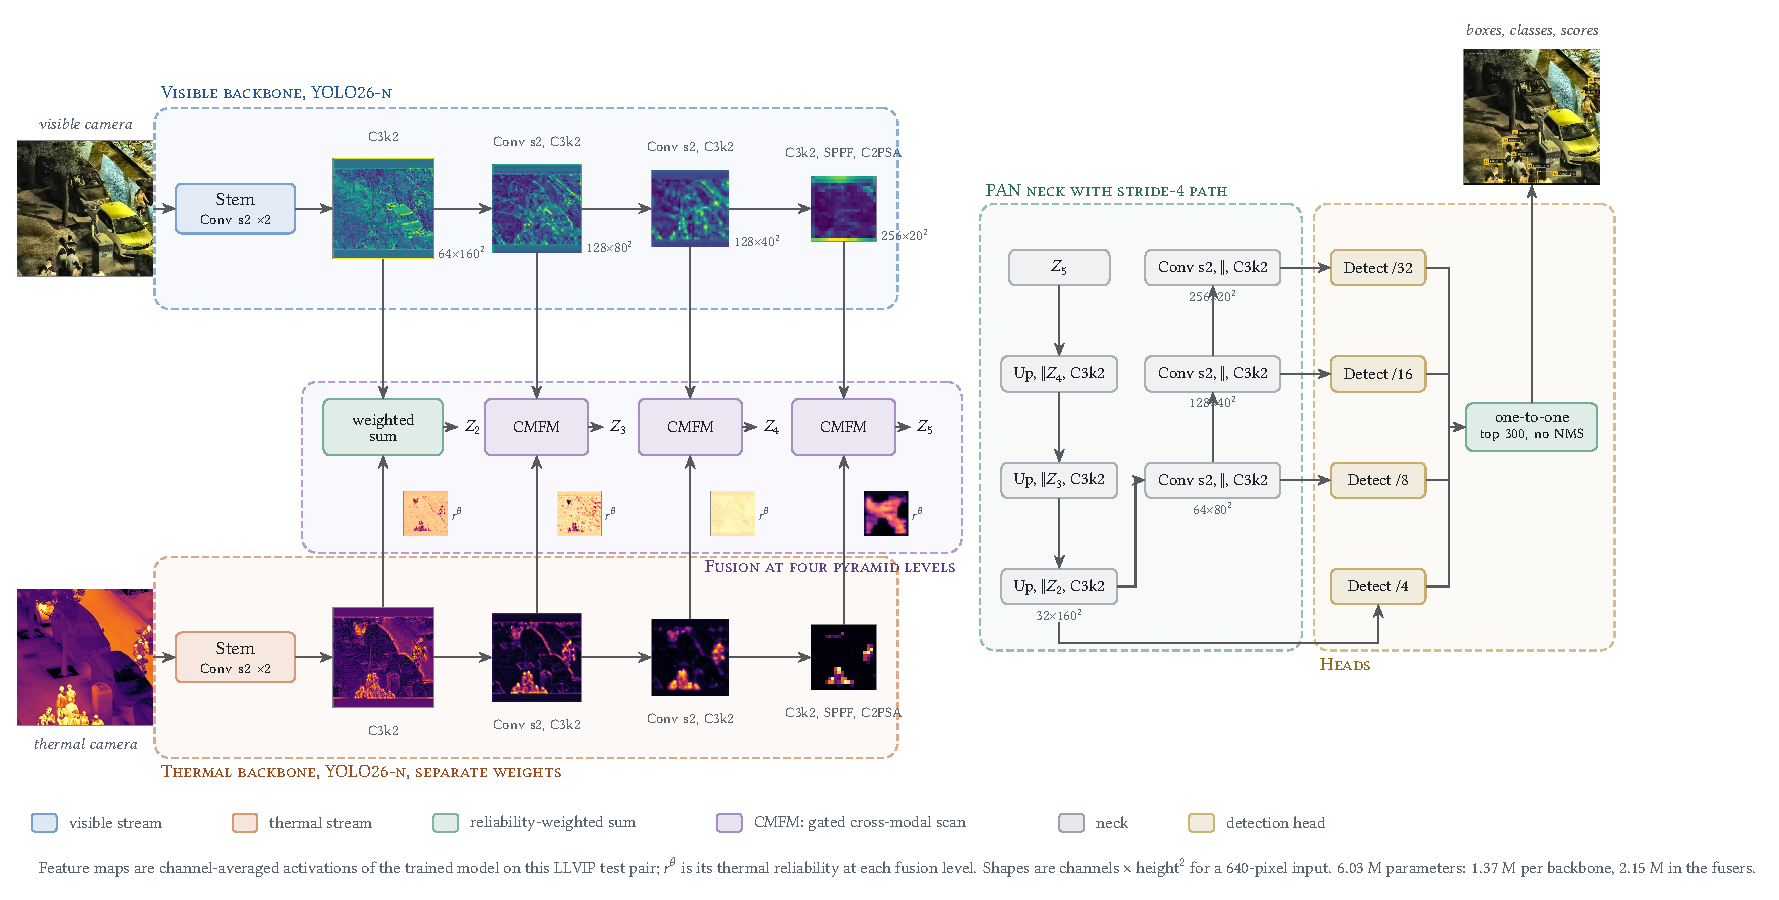
\includegraphics[width=\textwidth]{figures/fig_cffm_overall.pdf}
\caption{CFFM-Net v1 on a LLVIP pair. Two YOLO26-n backbones with separate weights are fused at each pyramid level; the neck and head are stock YOLO26. The thermal reliability $\rt$ is shown at each level. Versions v2 and v3 drop the stride-4 level and its detection head.}
\label{fig:overall}
\end{figure}

\section{Introduction}
\label{sec:intro}
\IEEEPARstart{A}{t} night a visible camera sees little and a thermal camera sees warm bodies without texture, so pairing the two is the standard answer for pedestrian and vehicle detection after dark. The pairing carries a cost that benchmark tables hide. Public paired datasets are curated so that both streams are present, registered and healthy in every frame. A deployed pair is none of those things for long. The visible camera is blinded by headlights or loses its exposure in a tunnel, the thermal core stalls during a shutter calibration, a lens knock shifts one image against the other, and a cable pull removes a stream entirely. A fusion network trained only on clean pairs has never been asked what to do when one input is wrong, and a detector that falls below its single-camera baseline in that moment is a worse sensor than either camera alone.

Recent fusion detectors build on selective state-space models~\cite{gu2023mamba}, which mix tokens along a sequence in linear time. Fusion-Mamba and CFMW scan the two modalities jointly and weight them afterwards~\cite{dong2025fusionmamba,li2025cfmw}; transformer fusers such as CFT and ICAFusion attend across modalities~\cite{fang2021cft,shen2024icafusion}. As far as their descriptions show, in each case the combination rule acts on features that a faulty camera has already shaped. In a selective scan the shaping happens early, because every token writes into a recurrent state through its own step size, and a corrupted token writes just as strongly as a clean one.

CFFM-Net (Cross-Feature Fusion Mamba Network) moves the decision to where the write happens. A small head predicts a reliability in $(0,1)$ for each camera at each location, and the scan multiplies the step size of a token by the reliability of the camera it came from. A token whose reliability is zero would have a zero step and leave the state untouched; in practice the fusion weight of a round-one model stays close to one half (Section~\ref{sec:gate}), so the learned reliability acts as a mild prior. The fusion block sits on top of a stock YOLO26 detector~\cite{yolo26_2026}, so the trainer, loss and evaluation are unchanged, and it is small enough to keep the whole detector at nano scale.

We present the detector, its baselines, ablations and a sensor-fault benchmark, a temporal extension evaluated on video, a live runtime, and the system built around them. The evidence is mixed in places, and we report it that way. Over three seeds the model beats a matched concatenation baseline on M3FD by \marMfdVtwoVsConcatMdMeanMap{}\,$\pm$\,\marMfdVtwoVsConcatMdStdMap{} mAP, which is not significant at $n=3$ (paired $p=\sigMfdP{}$), and is level with it on LLVIP and on KAIST still images. Fusing the two cameras beats the best single camera on M3FD by \gainMfdCffmVtwoOverBestMeanMap{}\,mAP, but the concatenation baseline captures \gainMfdConcatMdOverBestMeanMap{}\,of it. On the fault benchmark a baseline trained with fault augmentation is more robust than our model, which limits what the reliability gate can claim. In a preliminary single-seed run, a later variant with an auxiliary reliability loss is worse than the plain model, so the loss does not earn a place in the recipe. The contributions are as follows.
\begin{enumerate}
\item A cross-modal fusion block, CMFM, that gates the discretisation step of a four-direction selective scan by per-pixel, per-camera reliability, with a learned offset alignment and a convolutional local branch, built as a drop-in extension of YOLO26 (Section~\ref{sec:method}).
\item A controlled evaluation on LLVIP and M3FD with a matched baseline, three seeds, matched single-camera baselines on M3FD, size-banded average precision, and an eleven-fault sensor benchmark that includes a fault-trained baseline and the negative ablation of the reliability loss, set beside published results with their protocol differences stated (Section~\ref{sec:experiments}).
\item A Temporal State Memory that carries a per-pixel scan state across video frames, warped by frame-to-frame motion and slowed by the sensor reliability, and a live runtime with a stream health monitor that feeds sensor flags to the model (Sections~\ref{sec:tsm} and~\ref{sec:live}), evaluated on KAIST (Section~\ref{sec:video}) and in a soak and link-fault test on replayed streams (Section~\ref{sec:livexp}), where the memory helps under thermal noise and visible darkness and not under thermal loss or in tracking.
\item A multi-camera analytics layer on a ground plane, shown as an RGB-only system demonstration on WILDTRACK with a plain RGB detector and no fusion (Section~\ref{sec:system}).
\end{enumerate}
The remainder of the paper reviews related work, describes the method, reports the detection, video and live-runtime experiments, describes the system, and discusses limits. Section~\ref{sec:discussion} lists what the evidence does and does not support.

\section{Related Work}
\label{sec:related}
\subsection{Real-time detectors and small objects}
Real-time detection rests on feature pyramids~\cite{lin2017fpn} and path aggregation~\cite{liu2018panet}, and the YOLO family, most recently YOLO26~\cite{yolo26_2026} and its predecessor YOLO11~\cite{yolo11_2024}, packages both with a one-stage head. Small objects remain the acknowledged failure case. HPS-DETR reports that objects below ten pixels and distant objects are still missed~\cite{wang2025hpsdetr}, and CFMW reports that small objects are still its weak point~\cite{li2025cfmw}. We therefore report average precision by size band, rather than a single mAP, throughout.

\subsection{State-space models in vision}
Mamba makes the state-space step input dependent~\cite{gu2023mamba}. Vision variants differ mainly in how they order two-dimensional tokens: bidirectional scans~\cite{zhu2024vim}, cross scans over four directions~\cite{liu2024vmamba}, and hybrids that place Mamba and attention at different depths~\cite{hatamizadeh2025mambavision}. Mamba YOLO brings the idea into a YOLO detector~\cite{wang2025mambayolo}, and UAVDet pairs convolution with Mamba for small objects in aerial imagery~\cite{yang2026uavdet}. UAVDet states that the sequential state update uses GPU parallelism poorly, and CFMW reports a large rise in computation from its scan. Our scan uses the four-direction order of VMamba and keeps the state small (state size \cfgDState{}), and our cost results in Section~\ref{sec:cost} quantify the price.

\subsection{Visible-thermal object detection}
Multispectral pedestrian detection grew up on KAIST~\cite{hwang2015kaist}, where early work compared where in a network the two streams should meet~\cite{liu2016halfway} and added a segmentation branch to the detector~\cite{li2018msdsrcnn}. Later work in this line addressed misalignment between the two cameras, with a weakly aligned cross-modal learner~\cite{zhang2019arcnn}, and built interaction and guidance modules on two-stream convolutional detectors, namely cross-modality interactive attention~\cite{zhang2019cian}, guided attentive fusion~\cite{zhang2021gaff} and channel switching with spatial attention~\cite{cao2023csaa}. More recent detectors on KAIST, LLVIP and M3FD fall into three groups. Transformer fusers attend across the two modalities inside a YOLO-style or two-stage detector: CFT~\cite{fang2021cft} and ICAFusion~\cite{shen2024icafusion}, and IRDFusion with iterative relation-map differences~\cite{shen2025irdfusion}. Detection transformers adapt the DETR family to two inputs, as in MS-DETR~\cite{xing2024msdetr}, DAMSDet~\cite{guo2024damsdet} and GM-DETR~\cite{xiao2024gmdetr}. Other designs change the pipeline around the detector: a single-stage multispectral framework built on YOLOv11~\cite{wan2025yolov11rgbt}, a target-aware fusion for pedestrians~\cite{zhang2024tfdet}, an end-to-end design that trains image fusion and detection together~\cite{zhang2024e2emfd}, and a coarse-to-fine removal and selection scheme~\cite{zhao2026rsdet}. Remote-sensing detectors such as SuperYOLO and its relatives pair multispectral inputs with YOLO-style heads~\cite{zhang2023superyolo,fang2022yolofusion}. We compare with the published numbers of several of these in Section~\ref{sec:sota} and do not re-run them.

State-space fusion has appeared in this setting recently. Fusion-Mamba builds cross-modality fusion modules from state-space blocks~\cite{dong2025fusionmamba}, CFMW targets adverse weather~\cite{li2025cfmw}, WaveMamba applies a wavelet-driven Mamba fusion~\cite{zhu2025wavemamba}, and DMM uses disparity guidance for oriented objects in remote sensing~\cite{zhou2024dmm}. As far as their titles and abstracts show, these designs use the scan to mix the two modalities; we did not find one that gates the step of the scan by a per-camera reliability. MambaST fuses a few consecutive frames of a visible-thermal pair for pedestrian detection~\cite{mambast2024}; our Temporal State Memory differs in carrying a recurrent state indefinitely and in tying its decay to sensor reliability and real elapsed time.

\subsection{Reliability, illumination and modality imbalance}
The idea that one camera can be less trustworthy than the other is not new. MBNet argues that multispectral detectors suffer from modality imbalance and uses illumination information to align and weight the two feature streams~\cite{zhou2020mbnet}, and MS-DETR adds a modality-balanced optimisation to its loosely coupled fusion~\cite{xing2024msdetr}. Explicit attention across the two modalities has been proposed for several RGB-thermal tasks~\cite{liang2023eaefnet}, and probabilistic ensembling fuses the outputs of per-modality detectors~\cite{chen2022proben}. In the works we surveyed, reliability or illumination weights the modalities on the features or on the output of the fusion. We found no method that controls the discretisation step of the scan itself per location and per modality, which is the design choice we test. In the works we surveyed we also found no benchmark that corrupts one camera of a pair with a range of physical faults, which is why Section~\ref{sec:experiments} builds one.

\subsection{Datasets and tracking}
LLVIP provides registered visible-infrared pairs for low-light pedestrian detection~\cite{jia2021llvip}, and M3FD offers multiple scenarios and classes~\cite{liu2022tardal}. KAIST is the classic multispectral pedestrian benchmark, with sanitised annotations available~\cite{li2018kaistsanitized}, and its numbers depend strongly on whether training and test annotations are original or sanitised~\cite{zhang2021gaff}. A bag-of-tricks study benchmarks training choices for multispectral detectors~\cite{zhou2024tricks}. WILDTRACK supplies calibrated, synchronised multi-camera video of pedestrians~\cite{chavdarova2018wildtrack}. For tracking by detection we use ByteTrack, which associates low-confidence boxes as well as confident ones~\cite{zhang2022bytetrack}.

\section{Method}
\label{sec:method}
\subsection{Detector and notation}
CFFM-Net extends YOLO26-n. A pair enters as a four-channel tensor, visible BGR and one thermal grey channel, and the thermal channel is repeated to three for its backbone. Two backbones with separate weights, both initialised from COCO-pretrained YOLO26-n, produce feature maps at each pyramid level that the head reads. A fuser at each of those levels combines the visible map $\Fv$ and the thermal map $\Ft$ into one map $Z$ of the same shape, and the stock YOLO26 neck and one-to-one head consume the fused maps. Because the model subclasses the Ultralytics detection model and keeps the loss and validator unchanged, every result below comes from the standard trainer and the standard COCO-style evaluation. Figure~\ref{fig:overall} shows the layout.

Feature maps have $c$ channels and $h\times w$ cells at the level in question. Reliabilities $\rv,\rt\in(0,1)^{h\times w}$ are single-channel maps.

\subsection{Reliability head}
For each level, a head predicts how far each camera can be trusted at each cell from the evidence in both maps:
\begin{equation}
[\rv,\rt]=\sigma\!\Big(W_r\,\phi\big([\Fv,\;\Ft,\;|\Fv-\Ft|]\big)\Big),
\end{equation}
where $\phi$ is a depthwise $3{\times}3$ convolution with batch normalisation and SiLU, $W_r$ is a $1{\times}1$ convolution to two channels, and $\sigma$ is the logistic function. $W_r$ starts at zero weight with a bias of \cfgInitBias{}, so both cameras are trusted at initialisation. The absolute difference gives the head a direct view of disagreement between the cameras. An optional sensor flag $f\in\{0,1\}^2$ per sample multiplies the output, which is how an external monitor can declare a camera dead: the flag forces that camera's reliability to zero everywhere.

\subsection{Offset alignment}
Thermal and visible images are registered in LLVIP but not perfectly in the field. Before the scan, a small convolutional head predicts a two-channel displacement $\Delta=\delta_{\max}\tanh(g([\Fv,\Ft]))$ with $\delta_{\max}=\cfgMaxDisp{}$ cells, and bilinear sampling resamples the thermal map at the displaced positions, giving $\tilde F^{\theta}$. The output layer of $g$ starts at zero, so the block starts as the identity warp and learns a shift only if the loss rewards it.

\subsection{Reliability-gated cross scan}
Both maps are projected to $d=\max(16,\mathrm{round}(\cfgRatio{}\,c))$ channels by a $1{\times}1$ convolution followed by a depthwise $3{\times}3$ convolution, giving $p^{v}$ and $p^{\theta}$. At every cell the visible and thermal tokens are placed next to each other, so a sequence of $L=2hw$ tokens alternates $p^{v}_1,p^{\theta}_1,p^{v}_2,p^{\theta}_2,\dots$ over the raster order. The block scans this sequence in $K=\cfgDirections{}$ orders: rows forward and backward, columns forward and backward. For one direction, token $u_\ell$ with modality $m(\ell)\in\{v,\theta\}$ and grid position $\mathrm{pos}(\ell)$, the recurrence is
\begin{align}
\Delta_\ell &= \softplus\!\big(W_\Delta u_\ell + b_\Delta\big)\,\cdot\, r^{m(\ell)}_{\mathrm{pos}(\ell)},\\
h_\ell &= e^{\Delta_\ell A}\, h_{\ell-1} + \Delta_\ell\, B_\ell\, u_\ell,\\
y_\ell &= C_\ell\, h_\ell + D\, u_\ell,
\end{align}
with $A$ a diagonal matrix of negative entries (state size \cfgDState{}), and $B_\ell$, $C_\ell$ and the pre-activation of $\Delta_\ell$ produced from the token by learned projections, as in Mamba~\cite{gu2023mamba}. The only change from a standard selective scan is the last factor in the first line, the reliability at the token's position for the token's own camera. When that reliability is zero, $\Delta_\ell=0$, the decay factor is one, the input term vanishes, and the state passes the token untouched. A camera with zero reliability therefore cannot alter what the scan carries forward. The outputs of the four directions are mapped back to the grid and summed (Fig.~\ref{fig:scan}).

\begin{figure}[t]
\centering
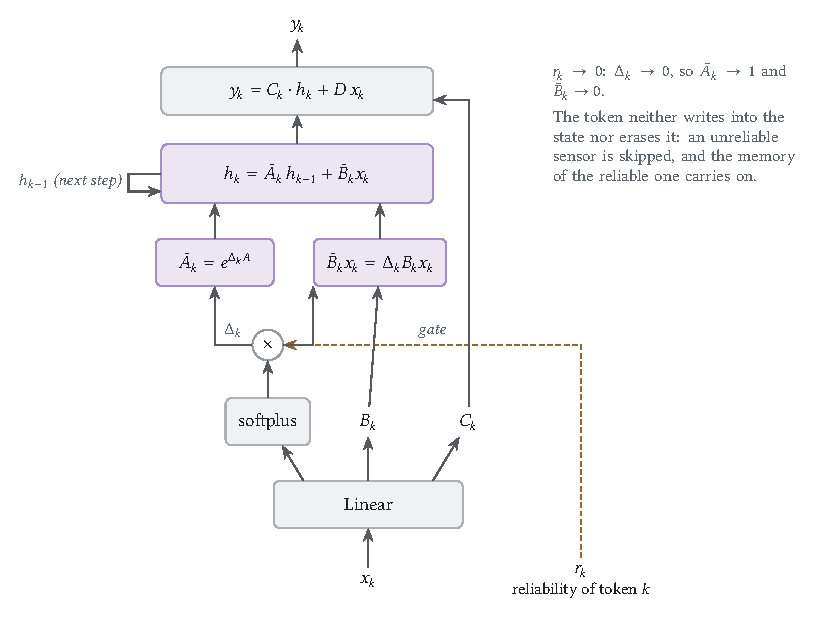
\includegraphics[width=0.8\columnwidth]{figures/fig_gated_scan.pdf}
\caption{One step of the gated scan. The reliability of the token's camera multiplies the step $\Delta_k$ before it enters the decay and the input term, so a reliability near zero leaves the state unchanged.}
\label{fig:scan}
\end{figure}

\subsection{CMFM and fusion levels}
The Cross-Modal Fusion Mamba block (CMFM) wraps the scan with two further paths. The scanned outputs of both modalities are concatenated and normalised by a channel LayerNorm. A local branch applies a depthwise $3{\times}3$ convolution to the concatenation of $p^{v}$ and $p^{\theta}$ and restores the two-dimensional neighbourhood that a one-dimensional scan weakens. A $1{\times}1$ convolution on the concatenation of both paths gives a residual $M$, and the block outputs
\begin{equation}
Z=\frac{\rv\,\Fv+\rt\,\tilde F^{\theta}}{\max(\rv+\rt,\,\cfgWeightFloor{})}+M.
\end{equation}
The projection producing $M$ starts at zero, so a freshly built block is exactly a reliability-weighted average of the two maps, and the scan has to earn any change. The weight floor keeps the gradient of the quotient bounded when both reliabilities approach zero. The scan runs in single precision. Three interchangeable scan implementations share one interface: a fused CUDA kernel when available, a fused Triton kernel, and a chunked two-pass PyTorch scan that serves as the reference and runs on any device.

The cost of the scan grows linearly in the number of cells, the number of directions, the channel width and the state size, and it is sequential along each of the $2hw$ tokens, which is why the stride-4 level is excluded from it. The implementation is covered by tests that check four properties: the chunked PyTorch scan equals the textbook recurrence in values and gradients; a token with zero step cannot write into the state; a freshly built CMFM is exactly a reliability-weighted average; and the offset alignment is the identity at initialisation.

Figure~\ref{fig:cmfm} shows the block. The detector fuses at the strides that its head reads. In the first version (v1) this is four levels: a reliability-weighted average at stride 4, where a scan over $2hw$ tokens is expensive and buys little, and CMFM at strides 8, 16 and 32. Versions v2 and v3 read the head at strides 8, 16 and 32 only. The baseline replaces every fuser by concatenation followed by a $1{\times}1$ convolution that squeezes the channels back to $c$, the usual two-stream design.

\begin{figure}[t]
\centering
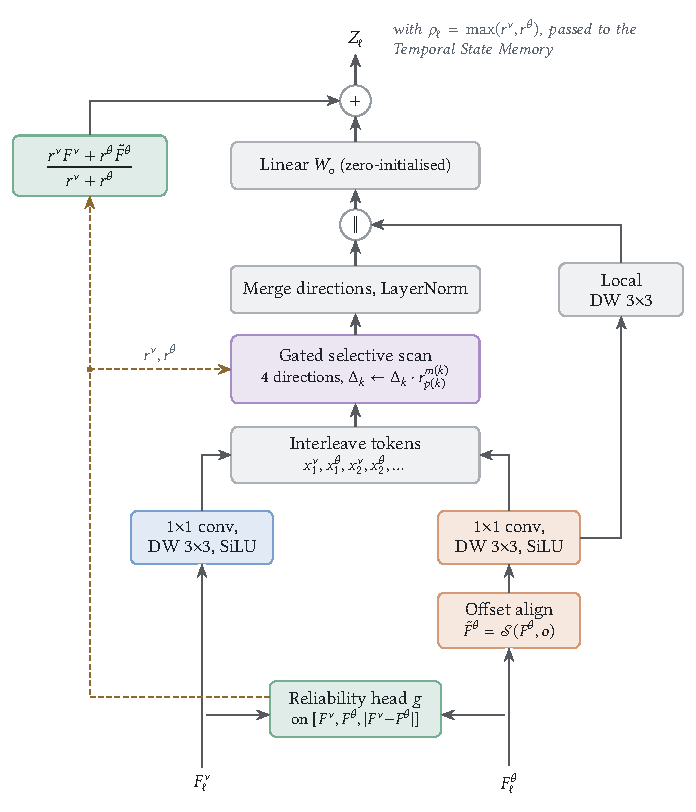
\includegraphics[width=0.78\columnwidth]{figures/fig_cmfm.pdf}
\caption{The CMFM block. A reliability head weights each camera, thermal features are warped onto the visible grid, visible and thermal tokens are interleaved and scanned in four directions with the step scaled by reliability, and a local convolution branch joins before a zero-initialised projection. The result adds to a reliability-weighted average. The larger of the two reliabilities is also passed to the temporal memory.}
\label{fig:cmfm}
\end{figure}

\subsection{Training recipes}
\label{sec:recipes}
Three recipes are compared; they differ in head layout and in what the training batches look like.
\begin{itemize}
\item \textbf{v1.} Four fusion levels, clean pairs only. It is the round-one model.
\item \textbf{v2.} Three levels and \emph{modality dropout}: each training pair has probability \cfgMdProb{} of having its visible camera blacked out, and the same probability for the thermal camera. For half of the blacked-out samples the model also receives the sensor flag. The control baseline is trained with the same dropout, so the comparison isolates the fuser.
\item \textbf{v3.} v2 plus \emph{fault training} and a \emph{reliability loss}. With probability \cfgFaultProb{} a sample has one random camera corrupted by one of the faults of the benchmark below at a random severity, and the head receives a trust target for that camera of \cfgTrustOne{}, \cfgTrustTwo{} or \cfgTrustThree{} at severity one, two or three, and zero for a blacked-out camera (healthy cameras have target one). The reliability loss is the binary cross-entropy between the mean reliability of each gated fuser and its trust target, averaged over fusers and added with weight \cfgRelWeight{}. The ablation \emph{v3 without reliability branch} keeps the fault training and removes the loss; the \emph{fault-trained concat} baseline keeps the fault training and the concat fuser.
\end{itemize}

\subsection{Temporal State Memory}
\label{sec:tsm}
A still-image detector forgets a pedestrian the moment its thermal camera drops a frame. The Temporal State Memory (TSM) gives each fusion level a per-pixel recurrent state that survives across frames. It is attached after the fuser at each level with a residual path that starts at zero, so a model with a fresh memory produces exactly the detections of the model without it (Fig.~\ref{fig:tsm}).

At frame $t$ the fused map $Z_t$ at one level is projected to $c_s=\mathrm{round}(\cfgMemRatio{}\,c)$ channels, $u_t=W_u Z_t$, and every channel at every cell keeps a state of size \cfgMemState{}. The update is a selective scan in time rather than space:
\begin{align}
\delta_t &= \softplus(W_\delta u_t)\cdot\frac{\tau_t}{\tau_0}\cdot\rho_t,\\
S_t &= e^{\delta_t A}\odot \mathcal{W}_{H_t}(S_{t-1}) + \delta_t\, B_t\, u_t,\\
y_t &= C_t\, S_t + D\, u_t,\qquad Z'_t = Z_t + W_o\,\mathrm{DW}(y_t),
\end{align}
where $B_t$ and $C_t$ come from $u_t$ by a $1{\times}1$ convolution, $\mathrm{DW}$ is a depthwise $3{\times}3$ convolution spreading the readout to neighbours, and $W_o$ is zero-initialised. Three factors act on the step. The ratio $\tau_t/\tau_0$ of the real time gap since the previous frame to a nominal gap $\tau_0=\cfgTauZero{}$\,s makes the decay depend on elapsed time, so a stalled camera that returns after a long gap forgets in proportion. The reliability $\rho_t=\max(\rv_t,\rt_t)$ from CMFM is high when at least one camera is trusted, and a frame in which neither camera is reliable writes little into the state. The warp $\mathcal{W}_{H_t}$ resamples the previous state under the homography $H_t$ from frame $t-1$ to $t$, with zeros for newly exposed cells, so the memory follows a moving camera rather than smearing. A scene cut, or a time gap beyond \cfgResetS{}\,s in the live runtime, resets the state.

The memory is trained with the detector frozen. Clips of \cfgClipLen{} frames at stride \cfgClipStride{} are drawn from KAIST training sequences~\cite{hwang2015kaist}, with labels for every frame. With probability one half a clip receives a fault, one of drop, darkness, noise, glare or shift, starting at a random frame and lasting to the end of the clip, which is the situation the memory exists for. The loss is the detection loss averaged over the frames of the clip, backpropagated through time, optimised with AdamW under a one-cycle schedule, with gradient clipping and with any non-finite step skipped.

\begin{figure*}[t]
\centering
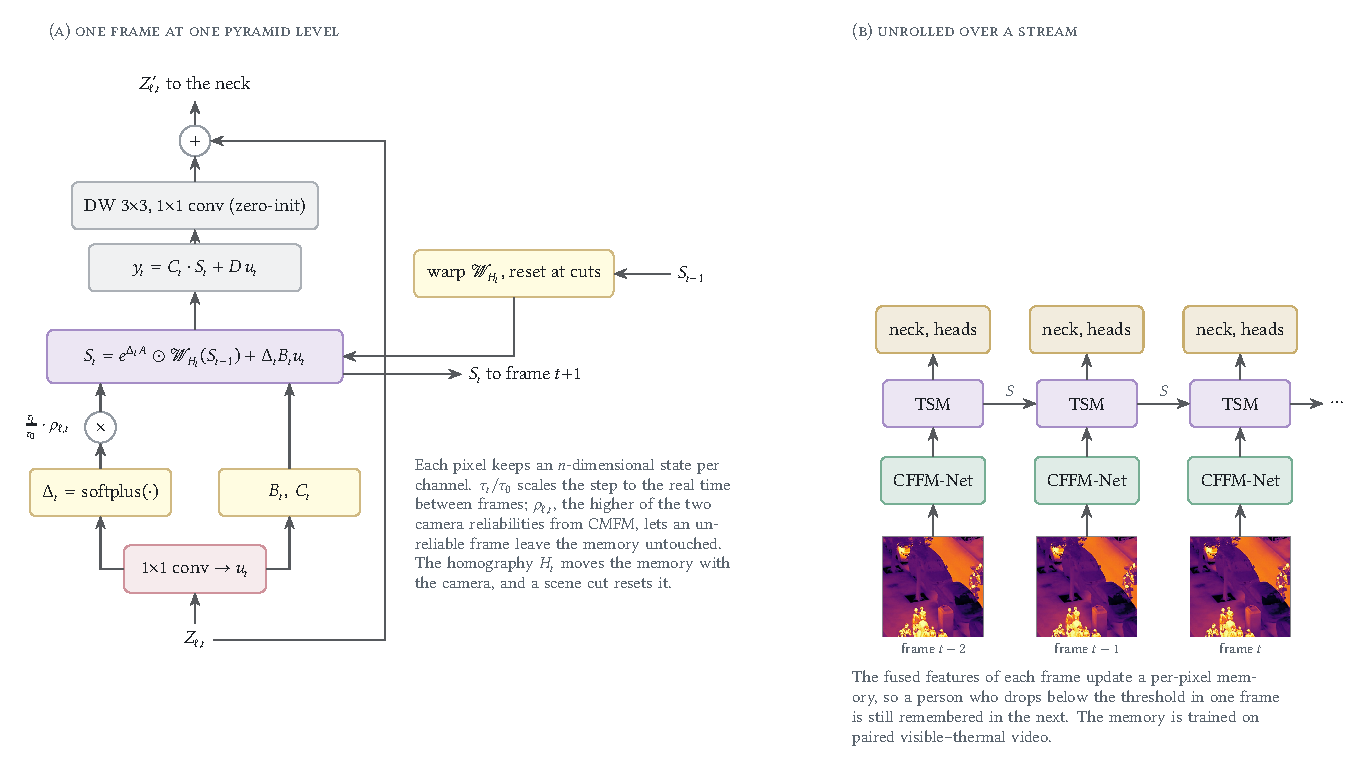
\includegraphics[width=0.82\textwidth]{figures/fig_tsm.pdf}
\caption{The Temporal State Memory. (a) One level at one frame: the step is scaled by elapsed time and by the camera reliability, and the previous state is warped by the frame-to-frame homography. (b) Unrolled over a stream, the memory sits between the fusion output and the neck.}
\label{fig:tsm}
\end{figure*}

\subsection{Causal inference and tracking on video}
\label{sec:causal}
Video inference is causal: frames are processed in order, the state is reset at the start of each sequence, and no future frame is used. For tracking, detections above a low confidence threshold feed ByteTrack~\cite{zhang2022bytetrack}, which also associates low-score boxes with existing tracks. Because the memory affects detections only, switching it off at test time gives the same model without memory, which is the ablation for video. A scheduler can inject a fault into a sequence, healthy for a number of frames and failed for the next number, repeating, to test recovery in the way a flaky link would behave. Detection is scored on KAIST by the log-average miss rate in the standard reasonable setting, split into day, night, failed and healthy frames, and tracking is scored by MOTA, IDF1 and identity switches against the KAIST person tracks.

\subsection{Live runtime}
\label{sec:live}
The live runtime turns the model into a process that reads two cameras and keeps running when they misbehave.

\paragraph{Capture}
Each camera runs in its own thread, stamps every frame with a monotonic time at the moment of capture, and writes it into a one-slot queue. A put replaces the frame waiting there and counts it as dropped, so a slow consumer never builds a backlog and latency cannot grow with time. A source that fails is reopened with backoff. Sources are a webcam index, an RTSP stream over TCP, or a replay of a recorded sequence at real speed with injected link faults: stalls, frozen frames, unplugs, random drops, delay and jitter.

\paragraph{Health monitor}
A monitor watches each camera from arrival times and pixels. It declares a camera stalled when no frame has arrived for \cfgStallIntervals{} nominal frame intervals, frozen when a downsampled frame has stayed nearly unchanged for \cfgFreezeFrames{} consecutive frames, black when the mean intensity is near zero, and saturated when a large share of pixels sits at the top of the range. Stalled, frozen and black cameras are \emph{down}, a saturated camera is \emph{degraded}, and others are \emph{ok}. The nominal rate is \cfgNominalFps{} frames per second.

\paragraph{Inference loop}
Each step takes the newest visible frame, waiting at most one frame interval, and the newest thermal frame without waiting, and reuses the last frame of a camera that has produced none. A camera that is down contributes a zero image and a zero sensor flag, which forces its reliability to zero everywhere, so the detector sees the failure as a stated fact rather than inferring it from a black picture. The gap between the timestamps of consecutive newest frames sets $\tau_t$ for the memory, and a gap longer than \cfgResetS{}\,s resets it. The model runs under half precision, followed by ByteTrack. Each step records inference time, end-to-end time from capture of the newest frame to the end of tracking, the time gap, the offset between the two camera timestamps, the health of each camera and the allocated GPU memory.

\paragraph{Summaries}
A run is summarised by throughput, median and 95th-percentile inference and end-to-end time, drift (the median end-to-end time over the last fifth of the run minus that over the first fifth), and growth in GPU memory. Fault handling is summarised by the delay from a fault's onset to the first \emph{down} status, the delay from its end to the first \emph{ok}, and the rate of false alarms.

\section{Experiments}
\label{sec:experiments}
\subsection{Setup}
\label{sec:setup}
\paragraph{Data}
LLVIP~\cite{jia2021llvip} is a registered visible-infrared set of pedestrians taken at night; we train on every \cfgLlvipStride{}rd frame of the training split and evaluate on the full test split. M3FD~\cite{liu2022tardal} has multiple scenarios and classes and no official detection split, so we hold out a fixed random \cfgMfdValPercent{}\,\% of the pairs with a seeded split that is shared by every run. Both datasets are converted to a four-channel paired layout, with images resized to \cfgImgsz{} pixels.

\paragraph{Models and training}
The baseline is the two-stream concatenation detector with the same backbones, neck and head, and matched training. Every fusion run uses COCO-pretrained YOLO26-n weights in both backbones, batch size \cfgBatch{}, and the stock Ultralytics trainer. Round one (v1) trains for \cfgEpochsPilot{} epochs on clean pairs and is run only for seed zero. All later rounds train for \cfgEpochs{} epochs with mosaic augmentation switched off for the last \cfgCloseMosaic{}. The headline comparison, v2 against the concat baseline with modality dropout, is run with \cfgSeedCount{} seeds on both datasets. The v3 family, its ablation and the fault-trained concat baseline are run with seed zero only, so v3 has no spread. The single-camera baselines are YOLO26-n detectors on one image stream, one seed. On M3FD they use the same pretrained weights, \cfgEpochs{} epochs and mosaic schedule as the fusion runs and a batch size of 32 instead of \cfgBatch{}; on LLVIP they were trained for \cfgEpochsPilot{} epochs and are not matched. Tables report percent as mean $\pm$ sample standard deviation over seeds ($n=3$), and margins are means of per-seed differences, in percentage points (pp). A printed margin can differ by a tenth from the difference of the printed means because the per-seed differences are not rounded first.

The five hypotheses tested in this work and their decision thresholds were fixed in advance, in the project plan of the repository, before the experiments ran.

\paragraph{Metrics}
We report COCO-style mAP at IoU 0.5 to 0.95 (mAP) and at 0.5 (mAP$_{50}$), and average precision for the COCO small, medium and large size bands. For M3FD we also report three finer bands from the AI-TOD convention, very tiny, tiny and small, which separate the smallest objects. Latency is batch one with \cfgLatH{}$\times$\cfgLatW{} input under half precision, after \cfgLatWarmup{} warm-up iterations and over \cfgLatIters{} timed iterations, from CUDA events.

\paragraph{Sensor-fault benchmark}
Eleven physically motivated faults are applied to one camera of the test pairs, each at three severities. The visible camera suffers darkness, glare, fog, noise, blur and a full drop; the thermal camera suffers a full drop, a spatial shift against the visible image, column banding with pixel noise, loss of contrast toward the scene mean (thermal crossover), and dead pixels. Severity three is the harshest and is the one reported. A drop has no severity, so its three levels coincide. In two further rows the dropped camera is declared to the model by the sensor flag. The benchmark scores v2 and the concat baseline with the checkpoints of all three seeds on M3FD and with the seed-zero checkpoints on LLVIP, whose seed-one and seed-two faults were not run. The fault-trained concat baseline is scored at seed zero on both datasets. Severity three is the one tabulated, and a seed contributes one value per fault.

\subsection{Main results}
\label{sec:main}
Table~\ref{tab:main} gives the headline comparison. On M3FD, CFFM-Net v2 reaches \resMfdCffmVtwoMeanMap{}\,$\pm$\,\resMfdCffmVtwoStdMap{} mAP against \resMfdConcatMdMeanMap{}\,$\pm$\,\resMfdConcatMdStdMap{} for the concat baseline, a margin of \marMfdVtwoVsConcatMdMeanMap{}\,$\pm$\,\marMfdVtwoVsConcatMdStdMap{}\,pp, and v2 is ahead on every one of the three seeds (Table~\ref{tab:seeds}). The margin is small and not significant at $n=3$: the paired $t$-test gives $p=\sigMfdP{}$ and the 95\,\% confidence interval of the margin is \sigMfdCiLow{} to \sigMfdCiHigh{}\,pp ($t_{0.975,2}=4.303$). Three wins out of three seeds have a one-sided sign-test probability of $\sigMfdSignP{}$ under no difference ($\sigMfdSignTwoSidedP{}$ two-sided), so the consistent sign is weak evidence. At IoU 0.5 the M3FD margin is \marMfdVtwoVsConcatMdMeanMapFifty{}\,$\pm$\,\marMfdVtwoVsConcatMdStdMapFifty{}\,pp.

On LLVIP the two models are level: \resLlvipCffmVtwoMeanMap{}\,$\pm$\,\resLlvipCffmVtwoStdMap{} for v2 against \resLlvipConcatMdMeanMap{}\,$\pm$\,\resLlvipConcatMdStdMap{}, a margin of \marLlvipVtwoVsConcatMdMeanMap{}\,$\pm$\,\marLlvipVtwoVsConcatMdStdMap{}\,pp whose spread exceeds its mean (paired $p=\sigLlvipP{}$, 95\,\% confidence interval \sigLlvipCiLow{} to \sigLlvipCiHigh{}\,pp). v2 is ahead on two of three seeds. We therefore read LLVIP as a tie and do not claim an LLVIP gain. LLVIP has one class and a thermal camera that already separates people from background, which leaves little room for a better fuser.

The single-camera rows give context. On M3FD the matched baselines reach \resMfdYoloVisSeedZeroMap{} mAP on the visible images and \resMfdYoloThmSeedZeroMap{} on the thermal images, so the visible camera is the stronger single camera there. Fusion beats it by a clear margin. CFFM-Net v2 is \gainMfdCffmVtwoOverBestMeanMap{}\,$\pm$\,\gainMfdCffmVtwoOverBestStdMap{}\,pp above the visible-only detector (\gainMfdCffmVtwoOverBestMinMap{}\,pp on its lowest seed) and the concat baseline is \gainMfdConcatMdOverBestMeanMap{}\,$\pm$\,\gainMfdConcatMdOverBestStdMap{}\,pp above it. At IoU 0.5 the v2 gain is \gainMfdCffmVtwoOverBestMapFiftyMean{}\,pp, and on small objects \gainMfdCffmVtwoOverBestApSmallMean{}\,pp. Most of the gain from fusing the two cameras on M3FD is thus available to the plain concat baseline, and the part that v2 adds is the margin of the previous paragraphs. Two caveats apply. The single-camera values are one seed, so the spread shown is that of the fusion side only and the true uncertainty of the gain is larger, and the single-camera batch size is twice the fusion batch size. On LLVIP the single-camera rows are not matched: \resLlvipYoloVisSeedZeroMap{} mAP for the visible images and \resLlvipYoloThmSeedZeroMap{} for the thermal ones, at \cfgEpochsPilot{} epochs and one seed against \cfgEpochs{} epochs for the fusion rows, so they support no conclusion about the gain from fusion there. At the round-one budget the concat baseline reaches \resLlvipConcatPlainSeedZeroMap{} and CFFM-Net v1 \resLlvipCffmVoneSeedZeroMap{}, and the round-one hypothesis that fusion beats the best single sensor at night came out inconclusive (\hypPhOneEvidence{}).

\begin{table}[t]
\centering
\caption{Detection accuracy in percent. Fusion models: mean and sample std over three seeds, 80 epochs. Single-camera rows: one seed; 30 epochs on LLVIP, which is not matched to the fusion rows, and 80 epochs on M3FD, which is. The margin over the best single camera subtracts the one-seed single-camera value from each fusion seed.}
\label{tab:main}
{\footnotesize\setlength{\tabcolsep}{4pt}
\adjustbox{max width=\linewidth}{\begin{tabular}{lcc}
\toprule
Model & mAP & mAP$_{50}$ \\
\midrule
\multicolumn{3}{l}{\emph{LLVIP}} \\
YOLO26-n visible & \resLlvipYoloVisSeedZeroMap & \resLlvipYoloVisSeedZeroMapFifty \\
YOLO26-n thermal & \resLlvipYoloThmSeedZeroMap & \resLlvipYoloThmSeedZeroMapFifty \\
Concat, modality dropout & \resLlvipConcatMdMeanMap\,\ensuremath{\pm}\,\resLlvipConcatMdStdMap & \resLlvipConcatMdMeanMapFifty\,\ensuremath{\pm}\,\resLlvipConcatMdStdMapFifty \\
CFFM-Net v2 & \resLlvipCffmVtwoMeanMap\,\ensuremath{\pm}\,\resLlvipCffmVtwoStdMap & \resLlvipCffmVtwoMeanMapFifty\,\ensuremath{\pm}\,\resLlvipCffmVtwoStdMapFifty \\
Margin of v2 over concat (pp) & \marLlvipVtwoVsConcatMdMeanMap\,\ensuremath{\pm}\,\marLlvipVtwoVsConcatMdStdMap & \marLlvipVtwoVsConcatMdMeanMapFifty\,\ensuremath{\pm}\,\marLlvipVtwoVsConcatMdStdMapFifty \\
\midrule
\multicolumn{3}{l}{\emph{M3FD}} \\
YOLO26-n visible & \resMfdYoloVisSeedZeroMap & \resMfdYoloVisSeedZeroMapFifty \\
YOLO26-n thermal & \resMfdYoloThmSeedZeroMap & \resMfdYoloThmSeedZeroMapFifty \\
Concat, modality dropout & \resMfdConcatMdMeanMap\,\ensuremath{\pm}\,\resMfdConcatMdStdMap & \resMfdConcatMdMeanMapFifty\,\ensuremath{\pm}\,\resMfdConcatMdStdMapFifty \\
CFFM-Net v2 & \resMfdCffmVtwoMeanMap\,\ensuremath{\pm}\,\resMfdCffmVtwoStdMap & \resMfdCffmVtwoMeanMapFifty\,\ensuremath{\pm}\,\resMfdCffmVtwoStdMapFifty \\
Margin of v2 over concat (pp) & \marMfdVtwoVsConcatMdMeanMap\,\ensuremath{\pm}\,\marMfdVtwoVsConcatMdStdMap & \marMfdVtwoVsConcatMdMeanMapFifty\,\ensuremath{\pm}\,\marMfdVtwoVsConcatMdStdMapFifty \\
Margin of v2 over best single camera (pp) & \gainMfdCffmVtwoOverBestMeanMap\,\ensuremath{\pm}\,\gainMfdCffmVtwoOverBestStdMap & \gainMfdCffmVtwoOverBestMapFiftyMean\,\ensuremath{\pm}\,\gainMfdCffmVtwoOverBestMapFiftyStd \\
\bottomrule
\end{tabular}}}
\end{table}


\subsection{Small objects}
\label{sec:small}
Table~\ref{tab:scale} separates the size bands. On M3FD, v2 gains on small objects, \marMfdVtwoVsConcatMdMeanApSmall{}\,$\pm$\,\marMfdVtwoVsConcatMdStdApSmall{}\,pp, medium objects are level (\marMfdVtwoVsConcatMdMeanApMedium{}\,$\pm$\,\marMfdVtwoVsConcatMdStdApMedium{}\,pp), and large objects gain \marMfdVtwoVsConcatMdMeanApLarge{}\,$\pm$\,\marMfdVtwoVsConcatMdStdApLarge{}\,pp with a spread larger than the mean. The small-object margin is the only band whose spread is smaller than its mean, and at $n=3$ it is not significant. The finer bands in Table~\ref{tab:bands} point the same way for the smallest objects, though the very tiny band is noisy: v2 reaches \resMfdCffmVtwoMeanApBandVeryTiny{}\,$\pm$\,\resMfdCffmVtwoStdApBandVeryTiny{} against \resMfdConcatMdMeanApBandVeryTiny{}\,$\pm$\,\resMfdConcatMdStdApBandVeryTiny{}, and in the tiny band \resMfdCffmVtwoMeanApBandTiny{}\,$\pm$\,\resMfdCffmVtwoStdApBandTiny{} against \resMfdConcatMdMeanApBandTiny{}\,$\pm$\,\resMfdConcatMdStdApBandTiny{}, whose baseline spread is wide.

On LLVIP the picture reverses at the small end. The margin of v2 on small objects is \marLlvipVtwoVsConcatMdMeanApSmall{}\,pp (spread \marLlvipVtwoVsConcatMdStdApSmall{}), while it gains \marLlvipVtwoVsConcatMdMeanApMedium{} and \marLlvipVtwoVsConcatMdMeanApLarge{}\,pp on medium and large ones. We do not claim a small-object advantage on LLVIP. The round-one model also failed the small-object hypothesis fixed in advance on M3FD: \hypPhThreeEvidence{}, verdict \hypPhThreeVerdict{}. The v2 gain therefore arrives only after the changes of Section~\ref{sec:recipes}, and the evidence for it is one dataset.

\begin{table}[t]
\centering
\caption{Average precision by object size in percent, mean and sample std over three seeds, 80 epochs.}
\label{tab:scale}
{\footnotesize\setlength{\tabcolsep}{4pt}
\adjustbox{max width=\linewidth}{\begin{tabular}{lccc}
\toprule
Model & Small & Medium & Large \\
\midrule
\multicolumn{4}{l}{\emph{LLVIP}} \\
Concat, modality dropout & \resLlvipConcatMdMeanApSmall\,\ensuremath{\pm}\,\resLlvipConcatMdStdApSmall & \resLlvipConcatMdMeanApMedium\,\ensuremath{\pm}\,\resLlvipConcatMdStdApMedium & \resLlvipConcatMdMeanApLarge\,\ensuremath{\pm}\,\resLlvipConcatMdStdApLarge \\
CFFM-Net v2 & \resLlvipCffmVtwoMeanApSmall\,\ensuremath{\pm}\,\resLlvipCffmVtwoStdApSmall & \resLlvipCffmVtwoMeanApMedium\,\ensuremath{\pm}\,\resLlvipCffmVtwoStdApMedium & \resLlvipCffmVtwoMeanApLarge\,\ensuremath{\pm}\,\resLlvipCffmVtwoStdApLarge \\
Margin of v2 (pp) & \marLlvipVtwoVsConcatMdMeanApSmall\,\ensuremath{\pm}\,\marLlvipVtwoVsConcatMdStdApSmall & \marLlvipVtwoVsConcatMdMeanApMedium\,\ensuremath{\pm}\,\marLlvipVtwoVsConcatMdStdApMedium & \marLlvipVtwoVsConcatMdMeanApLarge\,\ensuremath{\pm}\,\marLlvipVtwoVsConcatMdStdApLarge \\
\midrule
\multicolumn{4}{l}{\emph{M3FD}} \\
Concat, modality dropout & \resMfdConcatMdMeanApSmall\,\ensuremath{\pm}\,\resMfdConcatMdStdApSmall & \resMfdConcatMdMeanApMedium\,\ensuremath{\pm}\,\resMfdConcatMdStdApMedium & \resMfdConcatMdMeanApLarge\,\ensuremath{\pm}\,\resMfdConcatMdStdApLarge \\
CFFM-Net v2 & \resMfdCffmVtwoMeanApSmall\,\ensuremath{\pm}\,\resMfdCffmVtwoStdApSmall & \resMfdCffmVtwoMeanApMedium\,\ensuremath{\pm}\,\resMfdCffmVtwoStdApMedium & \resMfdCffmVtwoMeanApLarge\,\ensuremath{\pm}\,\resMfdCffmVtwoStdApLarge \\
Margin of v2 (pp) & \marMfdVtwoVsConcatMdMeanApSmall\,\ensuremath{\pm}\,\marMfdVtwoVsConcatMdStdApSmall & \marMfdVtwoVsConcatMdMeanApMedium\,\ensuremath{\pm}\,\marMfdVtwoVsConcatMdStdApMedium & \marMfdVtwoVsConcatMdMeanApLarge\,\ensuremath{\pm}\,\marMfdVtwoVsConcatMdStdApLarge \\
\bottomrule
\end{tabular}}}
\end{table}


\subsection{Sensor faults}
\label{sec:faults}
Table~\ref{tab:fault} reports the benchmark. On M3FD every number for v2 and the modality-dropout concat baseline is a mean over three seeds; on LLVIP it is one seed, and seed-to-seed spread of clean mAP there is about one point (Table~\ref{tab:seeds}), so LLVIP differences of one to three points are within seed noise. Faults on one camera cost every detector a large part of its mAP. Averaged over the eleven faults, v2 keeps \fltMfdCffmVtwoMeanRetainedSevThreePercent{}\,$\pm$\,\fltMfdCffmVtwoStdRetainedSevThreePercent{}\,\% of its clean mAP on M3FD against \fltMfdConcatMdMeanRetainedSevThreePercent{}\,$\pm$\,\fltMfdConcatMdStdRetainedSevThreePercent{}\,\% for the concat baseline, and \fltLlvipCffmVtwoRetainedSevThreePercent{}\,\% against \fltLlvipConcatMdRetainedSevThreePercent{}\,\% on LLVIP, where the baseline retains more. A thermal shift is the worst fault for every model on both datasets, and it leaves v2 \fltLlvipCffmVtwoWorstSevThreeMap{} mAP on LLVIP and \fltMfdCffmVtwoWorstSevThreeMap{} on M3FD.

The comparison between v2 and the concat baseline depends on the camera that fails (Fig.~\ref{fig:faultmargin}). On M3FD, v2 is ahead on every thermal-side fault: dead pixels by \fltMfdMarginThermalDeadSevThreeMeanMap{}\,pp, noise by \fltMfdMarginThermalNoiseSevThreeMeanMap{}, shift by \fltMfdMarginThermalShiftSevThreeMeanMap{}, crossover by \fltMfdMarginThermalCrossoverSevThreeMeanMap{} and a thermal drop by \fltMfdMarginThermalDropSevThreeMeanMap{}. It is behind on every visible-side fault, from \fltMfdMarginVisibleDarkSevThreeMeanMap{} (darkness) to \fltMfdMarginVisibleNoiseSevThreeMeanMap{}\,pp (noise). Averaged over the faults of each camera the margin is \fltMfdMarginMeanThermalAvgSevThreeMap{}\,$\pm$\,\fltMfdMarginStdThermalAvgSevThreeMap{}\,pp for thermal faults and \fltMfdMarginMeanVisibleAvgSevThreeMap{}\,$\pm$\,\fltMfdMarginStdVisibleAvgSevThreeMap{}\,pp for visible faults, and over all eleven it is \fltMfdMarginMeanAvgSevThreeMap{}\,$\pm$\,\fltMfdMarginStdAvgSevThreeMap{}\,pp (paired $p=\fltMfdMarginAvgP{}$ over the three seeds, 95\,\% interval \fltMfdMarginAvgCiLow{} to \fltMfdMarginAvgCiHigh{}\,pp), which is not significant at $n=3$. The sign of the per-fault margin agrees on all three seeds for \fltMfdSignAgreeSevThree{} of the \fltMfdFaultCount{} faults. The thermal-side advantage is consistent in direction, but the seed spread of single faults is large (for example $\pm$\fltMfdMarginThermalNoiseSevThreeStdMap{}\,pp on thermal noise), so we read it as a pattern the data support without a significance test passed. It is plausible for the design: when the thermal stream is degraded, the gate can lower its weight and the scan writes less of it into the state, while visible-side faults are corrupted before the visible features exist.

On LLVIP, with one seed, the benchmark is less kind. v2 is ahead on \fltLlvipWinsSevThree{} of the eleven faults, including darkness (\fltLlvipMarginVisibleDarkSevThreeMap{}\,pp), glare (\fltLlvipMarginVisibleGlareSevThreeMap{}), fog (\fltLlvipMarginVisibleFogSevThreeMap{}) and a visible drop (\fltLlvipMarginVisibleDropSevThreeMap{}), but it loses heavily to additive noise on either camera, by \fltLlvipMarginVisibleNoiseSevThreeMap{}\,pp on the visible side and \fltLlvipMarginThermalNoiseSevThreeMap{} on the thermal side, and to dead thermal pixels (\fltLlvipMarginThermalDeadSevThreeMap{}). The mean margin on LLVIP is \fltLlvipMarginAvgSevThreeMap{}\,pp. The gate is not a general robustness mechanism: it helps on specific faults, the thermal-side ones on M3FD and the exposure ones on LLVIP, and it hurts when noise is injected on LLVIP.

The strongest result of the benchmark concerns neither fusion design. A concat baseline trained with fault augmentation (Concat FT in Table~\ref{tab:fault}, seed zero) retains \fltMfdConcatFtRetainedSevThreePercent{}\,\% of its clean mAP on M3FD and \fltLlvipConcatFtRetainedSevThreePercent{}\,\% on LLVIP, against \fltMfdCffmVtwoMeanRetainedSevThreePercent{}\,\% and \fltLlvipCffmVtwoRetainedSevThreePercent{}\,\% for v2, and its mean mAP over the faults is higher than that of v2 by \fltMfdVtwoVsConcatFtGapSevThreeMap{}\,pp on M3FD and \fltLlvipVtwoVsConcatFtGapSevThreeMap{}\,pp on LLVIP, while its clean mAP is within one point of v2 (v2 minus Concat FT: \fltMfdVtwoVsConcatFtCleanMap{}\,pp on M3FD and \fltLlvipVtwoVsConcatFtCleanMap{}\,pp on LLVIP). Training on faulty inputs buys more robustness than the reliability-gated scan does, at no cost in clean accuracy. We did not run the fault benchmark on v3, which combines the scan with fault training, so we cannot say whether the scan adds anything once the training is matched; this is the comparison that would settle the value of the gate for robustness.

Telling the model which camera dropped through the sensor flag changes nothing measurable. The flagged and unflagged rows of Table~\ref{tab:fault} differ by at most two tenths of a point for every model, which suggests that detectors trained with modality dropout already recognise a black input without being told.

\begin{table*}[t]
\centering
\caption{Fault benchmark at severity three, mAP in percent, 80 epochs. LLVIP is seed 0 only. On M3FD the v2 and concat columns (modality dropout) are mean and sample std over three seeds, and the fault-trained concat column (Concat FT) is seed 0. Flagged rows tell the model which camera dropped.}
\label{tab:fault}
{\footnotesize\setlength{\tabcolsep}{4pt}
\adjustbox{max width=\linewidth}{\begin{tabular}{lcccccc}
\toprule
& \multicolumn{3}{c}{LLVIP, seed 0} & \multicolumn{3}{c}{M3FD, mean \ensuremath{\pm} std, three seeds} \\ \cmidrule(lr){2-4}\cmidrule(lr){5-7} Fault & v2 & Concat & Concat FT & v2 & Concat & Concat FT \\
\midrule
Clean & \fltLlvipCffmVtwoCleanMap & \fltLlvipConcatMdCleanMap & \fltLlvipConcatFtCleanMap & \fltMfdCffmVtwoCleanMeanMap\,\ensuremath{\pm}\,\fltMfdCffmVtwoCleanStdMap & \fltMfdConcatMdCleanMeanMap\,\ensuremath{\pm}\,\fltMfdConcatMdCleanStdMap & \fltMfdConcatFtCleanMap \\
\midrule
Visible dark & \fltLlvipCffmVtwoVisibleDarkThreeMap & \fltLlvipConcatMdVisibleDarkThreeMap & \fltLlvipConcatFtVisibleDarkThreeMap & \fltMfdCffmVtwoVisibleDarkThreeMeanMap\,\ensuremath{\pm}\,\fltMfdCffmVtwoVisibleDarkThreeStdMap & \fltMfdConcatMdVisibleDarkThreeMeanMap\,\ensuremath{\pm}\,\fltMfdConcatMdVisibleDarkThreeStdMap & \fltMfdConcatFtVisibleDarkThreeMap \\
Visible glare & \fltLlvipCffmVtwoVisibleGlareThreeMap & \fltLlvipConcatMdVisibleGlareThreeMap & \fltLlvipConcatFtVisibleGlareThreeMap & \fltMfdCffmVtwoVisibleGlareThreeMeanMap\,\ensuremath{\pm}\,\fltMfdCffmVtwoVisibleGlareThreeStdMap & \fltMfdConcatMdVisibleGlareThreeMeanMap\,\ensuremath{\pm}\,\fltMfdConcatMdVisibleGlareThreeStdMap & \fltMfdConcatFtVisibleGlareThreeMap \\
Visible fog & \fltLlvipCffmVtwoVisibleFogThreeMap & \fltLlvipConcatMdVisibleFogThreeMap & \fltLlvipConcatFtVisibleFogThreeMap & \fltMfdCffmVtwoVisibleFogThreeMeanMap\,\ensuremath{\pm}\,\fltMfdCffmVtwoVisibleFogThreeStdMap & \fltMfdConcatMdVisibleFogThreeMeanMap\,\ensuremath{\pm}\,\fltMfdConcatMdVisibleFogThreeStdMap & \fltMfdConcatFtVisibleFogThreeMap \\
Visible noise & \fltLlvipCffmVtwoVisibleNoiseThreeMap & \fltLlvipConcatMdVisibleNoiseThreeMap & \fltLlvipConcatFtVisibleNoiseThreeMap & \fltMfdCffmVtwoVisibleNoiseThreeMeanMap\,\ensuremath{\pm}\,\fltMfdCffmVtwoVisibleNoiseThreeStdMap & \fltMfdConcatMdVisibleNoiseThreeMeanMap\,\ensuremath{\pm}\,\fltMfdConcatMdVisibleNoiseThreeStdMap & \fltMfdConcatFtVisibleNoiseThreeMap \\
Visible blur & \fltLlvipCffmVtwoVisibleBlurThreeMap & \fltLlvipConcatMdVisibleBlurThreeMap & \fltLlvipConcatFtVisibleBlurThreeMap & \fltMfdCffmVtwoVisibleBlurThreeMeanMap\,\ensuremath{\pm}\,\fltMfdCffmVtwoVisibleBlurThreeStdMap & \fltMfdConcatMdVisibleBlurThreeMeanMap\,\ensuremath{\pm}\,\fltMfdConcatMdVisibleBlurThreeStdMap & \fltMfdConcatFtVisibleBlurThreeMap \\
Visible drop & \fltLlvipCffmVtwoVisibleDropThreeMap & \fltLlvipConcatMdVisibleDropThreeMap & \fltLlvipConcatFtVisibleDropThreeMap & \fltMfdCffmVtwoVisibleDropThreeMeanMap\,\ensuremath{\pm}\,\fltMfdCffmVtwoVisibleDropThreeStdMap & \fltMfdConcatMdVisibleDropThreeMeanMap\,\ensuremath{\pm}\,\fltMfdConcatMdVisibleDropThreeStdMap & \fltMfdConcatFtVisibleDropThreeMap \\
Thermal drop & \fltLlvipCffmVtwoThermalDropThreeMap & \fltLlvipConcatMdThermalDropThreeMap & \fltLlvipConcatFtThermalDropThreeMap & \fltMfdCffmVtwoThermalDropThreeMeanMap\,\ensuremath{\pm}\,\fltMfdCffmVtwoThermalDropThreeStdMap & \fltMfdConcatMdThermalDropThreeMeanMap\,\ensuremath{\pm}\,\fltMfdConcatMdThermalDropThreeStdMap & \fltMfdConcatFtThermalDropThreeMap \\
Thermal shift & \fltLlvipCffmVtwoThermalShiftThreeMap & \fltLlvipConcatMdThermalShiftThreeMap & \fltLlvipConcatFtThermalShiftThreeMap & \fltMfdCffmVtwoThermalShiftThreeMeanMap\,\ensuremath{\pm}\,\fltMfdCffmVtwoThermalShiftThreeStdMap & \fltMfdConcatMdThermalShiftThreeMeanMap\,\ensuremath{\pm}\,\fltMfdConcatMdThermalShiftThreeStdMap & \fltMfdConcatFtThermalShiftThreeMap \\
Thermal noise & \fltLlvipCffmVtwoThermalNoiseThreeMap & \fltLlvipConcatMdThermalNoiseThreeMap & \fltLlvipConcatFtThermalNoiseThreeMap & \fltMfdCffmVtwoThermalNoiseThreeMeanMap\,\ensuremath{\pm}\,\fltMfdCffmVtwoThermalNoiseThreeStdMap & \fltMfdConcatMdThermalNoiseThreeMeanMap\,\ensuremath{\pm}\,\fltMfdConcatMdThermalNoiseThreeStdMap & \fltMfdConcatFtThermalNoiseThreeMap \\
Thermal crossover & \fltLlvipCffmVtwoThermalCrossoverThreeMap & \fltLlvipConcatMdThermalCrossoverThreeMap & \fltLlvipConcatFtThermalCrossoverThreeMap & \fltMfdCffmVtwoThermalCrossoverThreeMeanMap\,\ensuremath{\pm}\,\fltMfdCffmVtwoThermalCrossoverThreeStdMap & \fltMfdConcatMdThermalCrossoverThreeMeanMap\,\ensuremath{\pm}\,\fltMfdConcatMdThermalCrossoverThreeStdMap & \fltMfdConcatFtThermalCrossoverThreeMap \\
Thermal dead & \fltLlvipCffmVtwoThermalDeadThreeMap & \fltLlvipConcatMdThermalDeadThreeMap & \fltLlvipConcatFtThermalDeadThreeMap & \fltMfdCffmVtwoThermalDeadThreeMeanMap\,\ensuremath{\pm}\,\fltMfdCffmVtwoThermalDeadThreeStdMap & \fltMfdConcatMdThermalDeadThreeMeanMap\,\ensuremath{\pm}\,\fltMfdConcatMdThermalDeadThreeStdMap & \fltMfdConcatFtThermalDeadThreeMap \\
Visible drop, flagged & \fltLlvipCffmVtwoVisibleDropThreeFlaggedMap & \fltLlvipConcatMdVisibleDropThreeFlaggedMap & \fltLlvipConcatFtVisibleDropThreeFlaggedMap & \fltMfdCffmVtwoVisibleDropThreeFlaggedMeanMap\,\ensuremath{\pm}\,\fltMfdCffmVtwoVisibleDropThreeFlaggedStdMap & \fltMfdConcatMdVisibleDropThreeFlaggedMeanMap\,\ensuremath{\pm}\,\fltMfdConcatMdVisibleDropThreeFlaggedStdMap & \fltMfdConcatFtVisibleDropThreeFlaggedMap \\
Thermal drop, flagged & \fltLlvipCffmVtwoThermalDropThreeFlaggedMap & \fltLlvipConcatMdThermalDropThreeFlaggedMap & \fltLlvipConcatFtThermalDropThreeFlaggedMap & \fltMfdCffmVtwoThermalDropThreeFlaggedMeanMap\,\ensuremath{\pm}\,\fltMfdCffmVtwoThermalDropThreeFlaggedStdMap & \fltMfdConcatMdThermalDropThreeFlaggedMeanMap\,\ensuremath{\pm}\,\fltMfdConcatMdThermalDropThreeFlaggedStdMap & \fltMfdConcatFtThermalDropThreeFlaggedMap \\
\midrule
Mean over faults & \fltLlvipCffmVtwoAvgSevThreeMap & \fltLlvipConcatMdAvgSevThreeMap & \fltLlvipConcatFtAvgSevThreeMap & \fltMfdCffmVtwoMeanAvgSevThreeMap\,\ensuremath{\pm}\,\fltMfdCffmVtwoStdAvgSevThreeMap & \fltMfdConcatMdMeanAvgSevThreeMap\,\ensuremath{\pm}\,\fltMfdConcatMdStdAvgSevThreeMap & \fltMfdConcatFtAvgSevThreeMap \\
Retained (\%) & \fltLlvipCffmVtwoRetainedSevThreePercent & \fltLlvipConcatMdRetainedSevThreePercent & \fltLlvipConcatFtRetainedSevThreePercent & \fltMfdCffmVtwoMeanRetainedSevThreePercent\,\ensuremath{\pm}\,\fltMfdCffmVtwoStdRetainedSevThreePercent & \fltMfdConcatMdMeanRetainedSevThreePercent\,\ensuremath{\pm}\,\fltMfdConcatMdStdRetainedSevThreePercent & \fltMfdConcatFtRetainedSevThreePercent \\
\bottomrule
\end{tabular}}}
\end{table*}


\begin{figure*}[t]
\centering
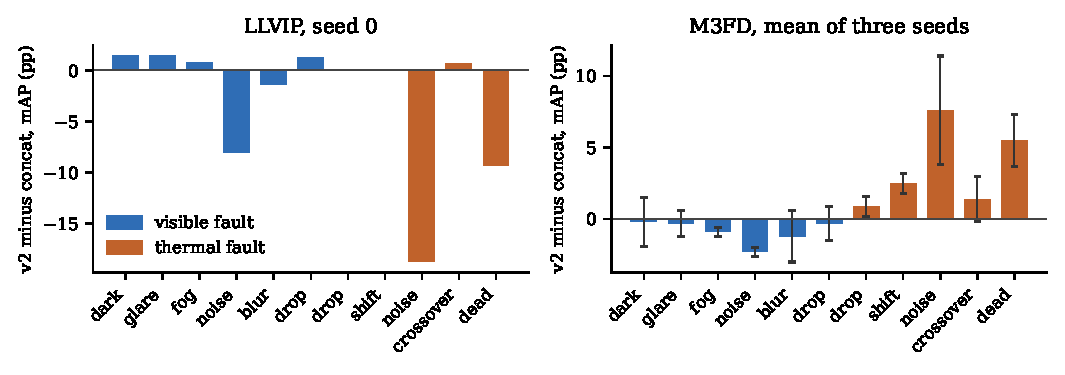
\includegraphics[width=0.85\textwidth]{figures/fig_fault_margin.pdf}
\caption{Margin of CFFM-Net v2 over the concat baseline for each fault at severity three, in mAP points, from Table~\ref{tab:fault}. Positive means v2 is ahead. LLVIP is one seed; M3FD shows the mean over three seeds with the sample standard deviation as an error bar.}
\label{fig:faultmargin}
\end{figure*}

\subsection{Ablations and the negative result}
\label{sec:ablation}
Table~\ref{tab:ablation} lists every variant and Table~\ref{tab:rounds} the margins over the control in each round. Three findings stand out.

First, round one was negative. CFFM-Net v1 had a margin of \marLlvipVoneVsConcatPlainSeedZeroMap{}\,pp on LLVIP and \marMfdVoneVsConcatPlainSeedZeroMap{}\,pp on M3FD against the concat baseline. Part of the gap came from the stride-4 level: adding that head lowers the concat baseline itself from \resLlvipConcatPlainSeedZeroMap{} to \resLlvipConcatPtwoSeedZeroMap{} on LLVIP, and against the concat baseline with the same head, the margin of v1 is \marLlvipVoneVsConcatPtwoSeedZeroMap{}\,pp. We took that as the reason to drop the stride-4 level in v2, a decision made on LLVIP at seed zero, since the P2 ablations were not run on M3FD. Removing the gate costs v1 \marLlvipVoneVsVoneNogateSeedZeroMap{}\,pp and replacing the scan by a gated convolution of matched cost \marLlvipVoneVsVoneGconvSeedZeroMap{}\,pp, both within the noise of one seed. We therefore do not claim that the scan or the gate, on their own, explain the v2 gain; the v2 comparison is between complete systems.

Second, v2 recovered the deficit. With three levels and modality dropout, shared by the baseline, v2 is level on LLVIP and ahead on M3FD.

Third, v3 failed in a preliminary, single-seed result. Adding fault training and the reliability loss gives \resLlvipCffmVthreeSeedZeroMap{} mAP on LLVIP and \resMfdCffmVthreeSeedZeroMap{} on M3FD, below v2 on both (\marLlvipVthreeVsVtwoSeedZeroMap{} and \marMfdVthreeVsVtwoSeedZeroMap{}\,pp) and below the fault-trained concat baseline (\marLlvipVthreeVsConcatFtSeedZeroMap{} and \marMfdVthreeVsConcatFtSeedZeroMap{}\,pp). The informative control is v3 without the reliability branch, which keeps the fault training and removes the loss. It reaches \resLlvipCffmVthreeNorelSeedZeroMap{} on LLVIP and \resMfdCffmVthreeNorelSeedZeroMap{} on M3FD and so v3 minus this control is \marLlvipVthreeVsVthreeNorelSeedZeroMap{} and \marMfdVthreeVsVthreeNorelSeedZeroMap{}\,pp: the branch costs accuracy. We therefore report the reliability loss as a negative ablation and do not include it in the recommended recipe. These are single-seed runs, so the size of the effect is uncertain, but the sign agrees on both datasets. A plausible cause is that the loss pushes the mean reliability toward a target that the detection loss does not need, and the two objectives compete. We did not test that explanation.

\begin{table}[t]
\centering
\caption{Ablation of mAP in percent. A dash marks a run that was not made.}
\label{tab:ablation}
{\footnotesize\setlength{\tabcolsep}{4pt}
\adjustbox{max width=\linewidth}{\begin{tabular}{lcc}
\toprule
Variant & LLVIP & M3FD \\
\midrule
\multicolumn{3}{l}{\emph{Round one, 30 epochs, seed 0}} \\
Two-stream concat & \resLlvipConcatPlainSeedZeroMap & \resMfdConcatPlainSeedZeroMap \\
CFFM-Net v1 & \resLlvipCffmVoneSeedZeroMap & \resMfdCffmVoneSeedZeroMap \\
v1, no gate & \resLlvipCffmVoneNogateSeedZeroMap & -- \\
v1, gated conv & \resLlvipCffmVoneGconvSeedZeroMap & -- \\
Concat + P2 head & \resLlvipConcatPtwoSeedZeroMap & -- \\
v1, no P2 head & \resLlvipCffmVoneNoptwoSeedZeroMap & -- \\
\midrule
\multicolumn{3}{l}{\emph{Rounds three and four, 80 epochs, seed 0}} \\
Concat, modality dropout & \resLlvipConcatMdSeedZeroMap & \resMfdConcatMdSeedZeroMap \\
CFFM-Net v2 & \resLlvipCffmVtwoSeedZeroMap & \resMfdCffmVtwoSeedZeroMap \\
Concat, fault training & \resLlvipConcatFtSeedZeroMap & \resMfdConcatFtSeedZeroMap \\
CFFM-Net v3 & \resLlvipCffmVthreeSeedZeroMap & \resMfdCffmVthreeSeedZeroMap \\
v3, no reliability branch & \resLlvipCffmVthreeNorelSeedZeroMap & \resMfdCffmVthreeNorelSeedZeroMap \\
\bottomrule
\end{tabular}}}
\end{table}

\begin{table}[t]
\centering
\caption{Round history: mAP margin of CFFM-Net over its control in percentage points.}
\label{tab:rounds}
{\footnotesize\setlength{\tabcolsep}{4pt}
\adjustbox{max width=\linewidth}{\begin{tabular}{p{0.6\columnwidth}cc}
\toprule
Comparison & LLVIP & M3FD \\
\midrule
Round one, v1 against concat (30 epochs) & \marLlvipVoneVsConcatPlainSeedZeroMap & \marMfdVoneVsConcatPlainSeedZeroMap \\
Head control, v1 without P2 against concat with P2 & \marLlvipVoneNoptwoVsConcatPtwoSeedZeroMap & -- \\
Round three, v2 against concat (seed 0) & \marLlvipVtwoVsConcatMdSeedZeroMap & \marMfdVtwoVsConcatMdSeedZeroMap \\
Round three, v2 against concat (three-seed mean) & \marLlvipVtwoVsConcatMdMeanMap & \marMfdVtwoVsConcatMdMeanMap \\
Round four, v3 against fault-trained concat & \marLlvipVthreeVsConcatFtSeedZeroMap & \marMfdVthreeVsConcatFtSeedZeroMap \\
Round four, v3 against v3 without reliability branch & \marLlvipVthreeVsVthreeNorelSeedZeroMap & \marMfdVthreeVsVthreeNorelSeedZeroMap \\
Round four, v3 against v2 & \marLlvipVthreeVsVtwoSeedZeroMap & \marMfdVthreeVsVtwoSeedZeroMap \\
\bottomrule
\end{tabular}}}
\end{table}


\subsection{Cost}
\label{sec:cost}
Table~\ref{tab:latency} gives the cost of the evaluated models on a \latLocalDevice{}, in half precision at batch one, timed on an otherwise idle GPU. CFFM-Net v2 has \latLocalVtwoParamsM{}\,M parameters and \latLocalVtwoGflops{} GFLOPs, a median latency of \latLocalVtwoMedianMs{}\,ms (about \latLocalVtwoFps{} frames per second) and a 95th percentile of \latLocalVtwoPNinetyFiveMs{}\,ms. Against the concat baseline this is \latLocalRatioParams{} times the parameters, \latLocalRatioGflops{} times the FLOPs, \latLocalRatioMedian{} times the median latency and \latLocalRatioPNinetyFive{} times the 95th-percentile latency, so v2 passes the limit of at most twice the baseline latency that was fixed in advance. Against the thermal-only detector the median latency is \latLocalVtwoOverThmMedian{} times higher. v3 and its no-branch control have the size of v2, and v3 is \latLocalVthreeOverVtwoMedian{} times the median latency of v2 in this run, so the timing differences between these three models are small and partly noise. The round-one model v1 was timed in an earlier session on hardware that is not recorded, at \latLlvipRatioMedian{} times the baseline; that run is not comparable with Table~\ref{tab:latency}. The gated-convolution control of matched FLOPs was faster than the scan in that run (\latLlvipCffmVoneGconvMedianMs{} against \latLlvipCffmVoneMedianMs{}\,ms), which is the price of a sequential scan on this kind of hardware.

\begin{table}[t]
\centering
\caption{Parameters (millions), GFLOPs and latency (ms) on a \latLocalDevice{}, half precision, batch one, \cfgLatW{}$\times$\cfgLatH{} input, median and 95th percentile per image over \cfgLatIters{} timed iterations after \cfgLatWarmup{} warm-up iterations, on an otherwise idle GPU.}
\label{tab:latency}
{\footnotesize\setlength{\tabcolsep}{4pt}
\adjustbox{max width=\linewidth}{\begin{tabular}{lrrrr}
\toprule
Model & Params & GFLOPs & Median & p95 \\
\midrule
YOLO26-n thermal only & \latLocalYoloThmParamsM & \latLocalYoloThmGflops & \latLocalYoloThmMedianMs & \latLocalYoloThmPNinetyFiveMs \\
Concat, modality dropout & \latLocalConcatMdParamsM & \latLocalConcatMdGflops & \latLocalConcatMdMedianMs & \latLocalConcatMdPNinetyFiveMs \\
Concat, fault training & \latLocalConcatFtParamsM & \latLocalConcatFtGflops & \latLocalConcatFtMedianMs & \latLocalConcatFtPNinetyFiveMs \\
CFFM-Net v2 & \latLocalVtwoParamsM & \latLocalVtwoGflops & \latLocalVtwoMedianMs & \latLocalVtwoPNinetyFiveMs \\
v3, no reliability branch & \latLocalVthreeNorelParamsM & \latLocalVthreeNorelGflops & \latLocalVthreeNorelMedianMs & \latLocalVthreeNorelPNinetyFiveMs \\
CFFM-Net v3 & \latLocalVthreeParamsM & \latLocalVthreeGflops & \latLocalVthreeMedianMs & \latLocalVthreePNinetyFiveMs \\
\midrule
v2 over concat, ratio & \latLocalRatioParams & \latLocalRatioGflops & \latLocalRatioMedian & \latLocalRatioPNinetyFive \\
\bottomrule
\end{tabular}}}
\end{table}


\subsection{Context with published detectors}
\label{sec:sota}
The experiments above compare CFFM-Net with a matched baseline and not with published fusion detectors, because published numbers differ in backbone, input size, training schedule, annotations and split. Tables~\ref{tab:sota} and~\ref{tab:sotakaist} nevertheless place our results next to those figures, copied from the cited papers and not re-run, so that a reader can see the distance. Our models are nano scale: CFFM-Net v2 has \latLocalVtwoParamsM{}\,M parameters and \latLocalVtwoGflops{} GFLOPs at $\cfgLatW{}\times\cfgLatH{}$, and runs at a median of \latLocalVtwoMedianMs{}\,ms on a laptop GPU. Most of the published detectors in the tables use YOLOv5-l, YOLOv8-l or ResNet-50 backbones, and several use detection transformers; we do not tabulate their sizes because we did not verify them against the original papers, and we make no claim about relative efficiency.

\begin{table*}[t]
\centering
\caption{Published RGB-T detection results for context, in percent. Numbers are copied from the cited papers, not re-run. Input size or split is stated per row because mAP depends on both. Our models are nano scale, trained on one third of the LLVIP training frames (mean of three seeds), so they are not a like-for-like comparison. On M3FD no row shares a split with ours, and no ranking is claimed.}
\label{tab:sota}
{\footnotesize\setlength{\tabcolsep}{4pt}
\adjustbox{max width=\linewidth}{\begin{tabular}{lllcc}
\toprule
Method & Detector & Input or split & mAP$_{50}$ & mAP \\
\midrule
\multicolumn{5}{l}{\emph{LLVIP, official split (12,025 / 3,463 pairs)}} \\
YOLOv5-l, infrared only~\cite{jia2021llvip} & YOLOv5-l & not stated & 96.5 & 67.0 \\
CFT~\cite{fang2021cft} & YOLOv5 with CFB & 640$\times$640 & 97.5 & 63.6 \\
CSSA~\cite{cao2023csaa} & Faster R-CNN, ResNet-50 & 640$\times$512 & 94.3 & 59.2 \\
MS-DETR~\cite{xing2024msdetr} & Deformable DETR, ResNet-50 & 640$\times$512 & 97.9 & 66.1 \\
Fusion-Mamba~\cite{dong2025fusionmamba} & YOLOv8-l & 640$\times$640 & 97.0 & 64.3 \\
DAMSDet~\cite{guo2024damsdet} & DETR, ResNet-50 & 1024$\times$1024 & 97.9 & 69.6 \\
TFDet~\cite{zhang2024tfdet} & YOLOv5-l & not stated & 97.9 & 71.1 \\
WaveMamba~\cite{zhu2025wavemamba} & YOLOv8 & not stated & 98.3 & 66.0 \\
IRDFusion~\cite{shen2025irdfusion} & Co-DETR & 640$\times$640 & 98.4 & 70.9 \\
CFFM-Net v2 (this work) & YOLO26-n, \latLocalVtwoParamsM{}\,M & \cfgImgsz{}, every third frame & \resLlvipCffmVtwoMeanMapFifty & \resLlvipCffmVtwoMeanMap \\
Concat baseline (this work) & YOLO26-n, \latLocalConcatMdParamsM{}\,M & \cfgImgsz{}, every third frame & \resLlvipConcatMdMeanMapFifty & \resLlvipConcatMdMeanMap \\
\midrule
\multicolumn{5}{l}{\emph{M3FD, splits differ between rows and are not comparable}} \\
TarDAL, fused image~\cite{liu2022tardal} & YOLOv5 & 3,500 train, test not stated & 80.7 & -- \\
DAMSDet~\cite{guo2024damsdet} & DETR, ResNet-50 & 3,368 / 831, by scene & 80.2 & 52.9 \\
TFDet~\cite{zhang2024tfdet} & YOLOv5 & 2,905 / 1,295 & 64.8 & 41.0 \\
E2E-MFD~\cite{zhang2024e2emfd} & Detectron2, end to end & 2,940 / 1,260 & 91.8 & 63.8 \\
Fusion-Mamba~\cite{dong2025fusionmamba} & YOLOv8-l & split of Liang et al. & 88.0 & 61.9 \\
WaveMamba~\cite{zhu2025wavemamba} & YOLOv8 & 3,360 / 840 & 92.1 & 64.4 \\
CFFM-Net v2 (this work) & YOLO26-n, \latLocalVtwoParamsM{}\,M & 3,360 / 840, random & \resMfdCffmVtwoMeanMapFifty & \resMfdCffmVtwoMeanMap \\
Concat baseline (this work) & YOLO26-n, \latLocalConcatMdParamsM{}\,M & 3,360 / 840, random & \resMfdConcatMdMeanMapFifty & \resMfdConcatMdMeanMap \\
\bottomrule
\end{tabular}}}
\end{table*}

\begin{table*}[t]
\centering
\caption{KAIST log-average miss rate in percent on the reasonable subset (lower is better). Published rows use the improved test annotations and the standard evaluation code and are copied from the cited papers. Our rows use the original annotations for training and testing, every 20th test frame and our own implementation of the protocol, so they are indicative only.}
\label{tab:sotakaist}
{\footnotesize\setlength{\tabcolsep}{4pt}
\adjustbox{max width=\linewidth}{\begin{tabular}{lllccc}
\toprule
Method & Detector & Train annotations & All & Day & Night \\
\midrule
AR-CNN~\cite{zhang2019arcnn} & VGG-16 & sanitized & 9.34 & 9.94 & 8.38 \\
MBNet~\cite{zhou2020mbnet} & ResNet-50 & AR-CNN improved & 8.13 & 8.28 & 7.86 \\
GAFF, original training~\cite{zhang2021gaff} & VGG-16 & original & 10.62 & 10.82 & 10.14 \\
GAFF, sanitized training~\cite{zhang2021gaff} & VGG-16 & sanitized & 6.48 & 8.35 & 3.46 \\
ICAFusion~\cite{shen2024icafusion} & YOLOv5, CSPDarknet53 & sanitized & 7.17 & 6.82 & 7.85 \\
MS-DETR~\cite{xing2024msdetr} & ResNet-50 & sanitized & 6.13 & 7.78 & 3.18 \\
TFDet~\cite{zhang2024tfdet} & VGG-16 & sanitized & 4.47 & 5.22 & 3.36 \\
\midrule
Concat baseline (this work) & YOLO26-n & original & \kstConcatAllMr & \kstConcatDayMr & \kstConcatNightMr \\
CFFM-Net v2 (this work) & YOLO26-n & original & \kstCffmAllMr & \kstCffmDayMr & \kstCffmNightMr \\
\bottomrule
\end{tabular}}}
\end{table*}


On LLVIP, with the official split, v2 reaches \resLlvipCffmVtwoMeanMapFifty{}\,\% mAP$_{50}$ and \resLlvipCffmVtwoMeanMap{}\,\% mAP, in the range of published fusion results (mAP from \sotaLlvipFusionMapMin{} to \sotaLlvipFusionMapMax{}) and below the best of them. This is with training on one third of the training frames and without a large backbone. The comparison is weaker than it looks. The LLVIP infrared-only baseline with a large YOLOv5 already reaches \sotaLlvipIrOnlyMap{} mAP in the dataset paper~\cite{jia2021llvip}, so thermal imagery alone nearly saturates the benchmark, and a gap of a few points of mAP between two fusion detectors at different input sizes (one row trains at a much larger input than the others) says little about the fuser. On M3FD no row shares our split. Published values of mAP$_{50}$ run from \sotaMfdMapFiftyMin{} to \sotaMfdMapFiftyMax{} across splits of the same dataset, and the same method (CFT) is reported \sotaMfdSplitSwing{} points of mAP$_{50}$ apart in two cited papers that use different splits, so we draw no ranking from the M3FD rows.

On KAIST our miss rates are far above the published ones (Table~\ref{tab:sotakaist}): \kstConcatAllMr{}\,\% for the concat baseline and \kstCffmAllMr{}\,\% for CFFM-Net v2 against \sotaKaistMrMin{} to \sotaKaistMrMax{} for the published detectors, which use ResNet or VGG backbones, sanitised training annotations and the standard evaluation code. We attribute part of the gap to the protocol differences in Section~\ref{sec:kaistprotocol} and part to scale and a short schedule, but we did not run the experiments that would apportion it, and the table should be read as showing that our KAIST detectors are not competitive with the published state of the art. The KAIST experiments serve the video questions of Section~\ref{sec:video} and not a leaderboard claim.

\subsection{What the gate learns}
\label{sec:gate}
Figure~\ref{fig:trust} plots, for LLVIP and M3FD test images, the share of fusion weight given to the thermal camera against the mean brightness of the visible image, for a round-one model. The share moves in the expected direction. In the darkest LLVIP scenes it leans toward thermal and in the brightest M3FD scenes toward visible. The swing is small, and the share stays close to one half everywhere. The gate at round one is therefore a mild prior and not a switch, which fits the modest gains above. Figure~\ref{fig:hero} shows the trust map on one night scene.

\begin{figure*}[t]
\centering
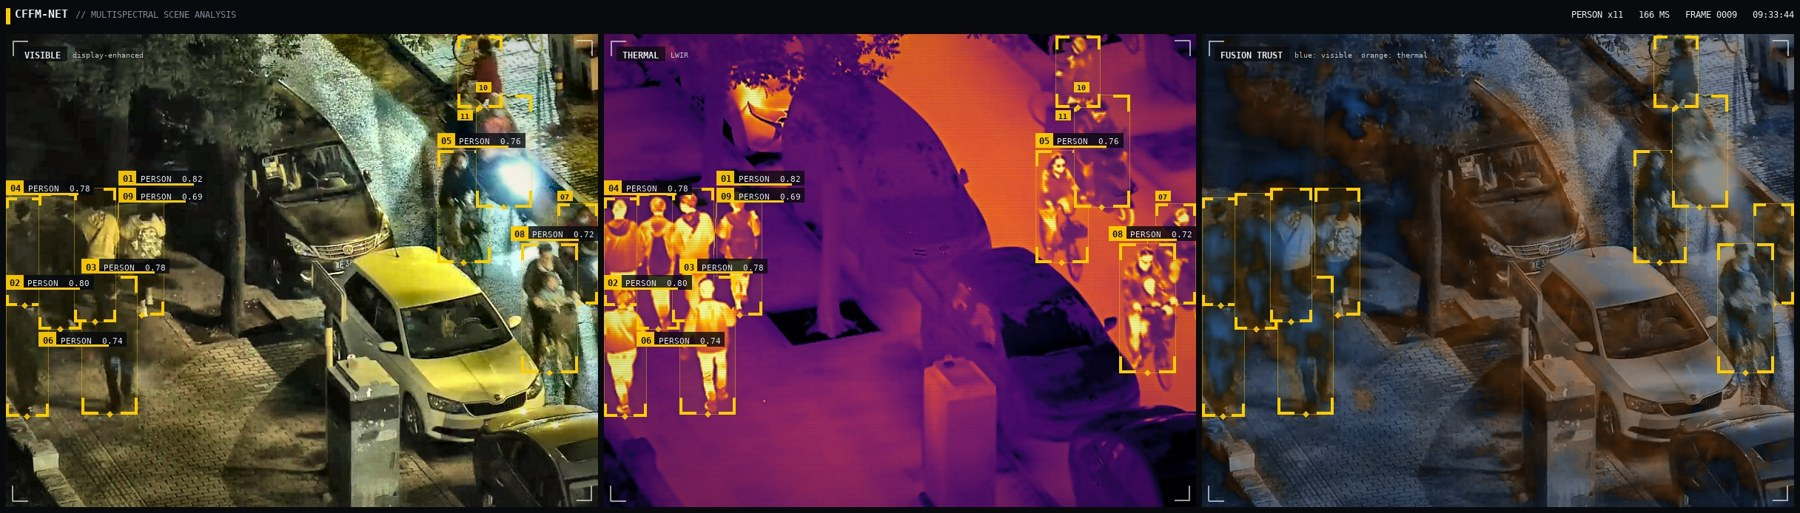
\includegraphics[width=0.9\textwidth]{figures/hero_llvip.jpg}
\caption{A LLVIP test pair as the round-one CFFM-Net sees it: visible with detections, thermal, and the fusion trust map in which blue marks visible and orange marks thermal weight.}
\label{fig:hero}
\end{figure*}

\begin{figure}[t]
\centering
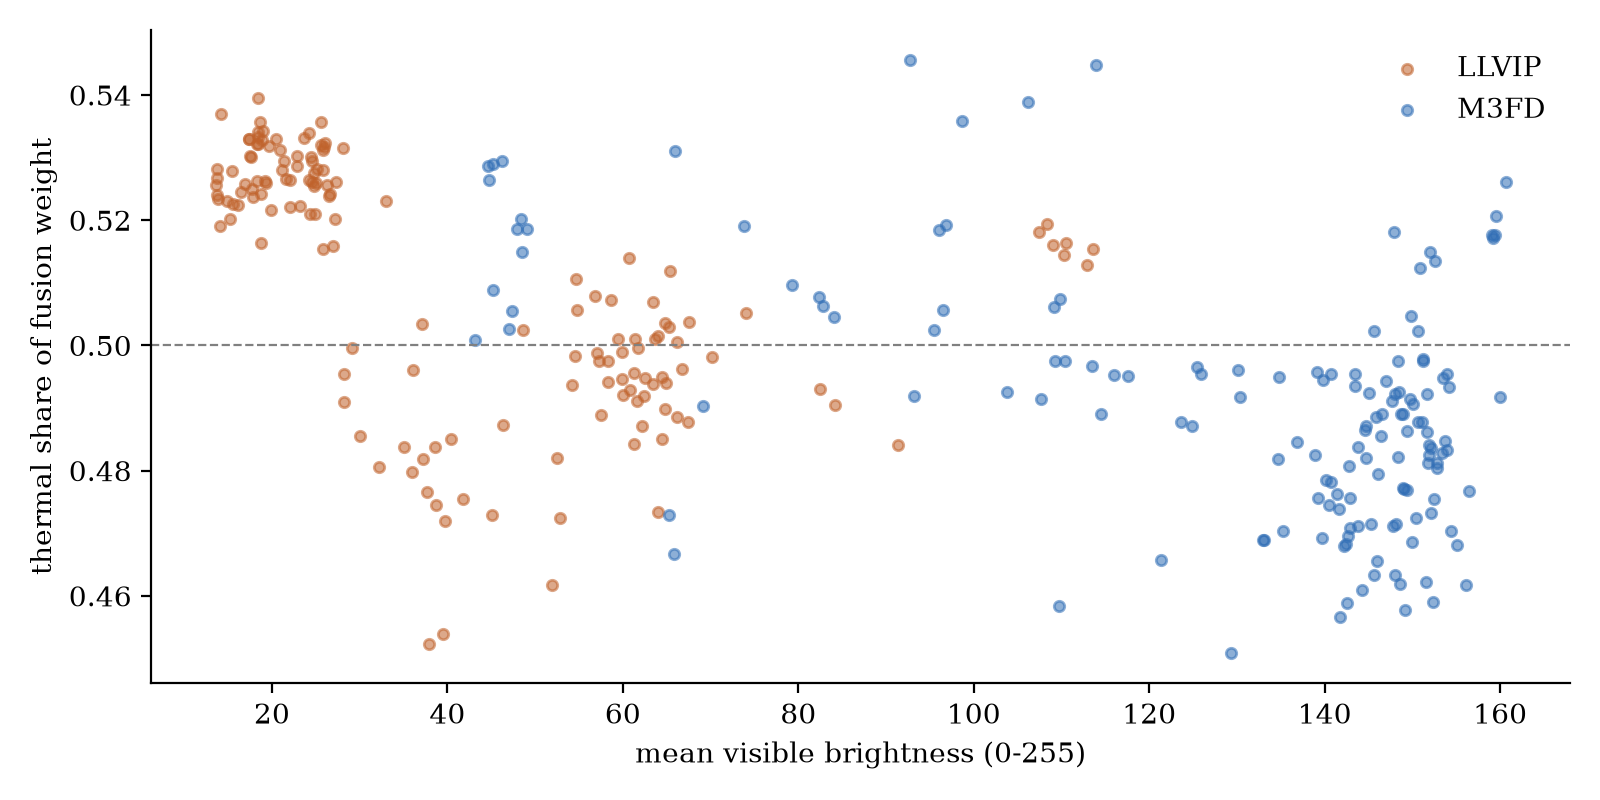
\includegraphics[width=\columnwidth]{figures/trust_vs_brightness.png}
\caption{Thermal share of the fusion weight against mean visible brightness for LLVIP and M3FD test images, with a round-one CFFM-Net. The dashed line marks an equal share.}
\label{fig:trust}
\end{figure}

\section{Video Experiments on KAIST}
\label{sec:video}
This section asks two questions about the video extension of Section~\ref{sec:tsm}. Does the fusion block help on a pedestrian benchmark with a long history of published results, and what does the Temporal State Memory add on top of a still-image detector, on clean video and while one camera fails? Every number here comes from one training run per model and one memory training run, so no seed spread is available, and we say so wherever a difference is small.

\subsection{Protocol}
\label{sec:kaistprotocol}
KAIST~\cite{hwang2015kaist} supplies visible and thermal video at 20 frames per second. We use the standard split: sets 00 to 05 for training and sets 06 to 11 for testing, with sets 00 to 02 and 06 to 08 recorded by day and the rest at night. The still-image detectors train on every \cfgKaistTrainStride{}th frame of the training sets, with persons at least \cfgKaistTrainMinH{} pixels tall as targets. Both detectors, CFFM-Net v2 and the concat baseline with modality dropout, follow the recipe of Section~\ref{sec:experiments} with \cfgKaistEpochs{} epochs and seed zero. The test frames are every \cfgKaistTestStride{}th frame of the test sets, \kstNAll{} frames of which \kstNDay{} are by day and \kstNNight{} by night.

The metric is the log-average miss rate (MR) over nine false-positives-per-image values between $10^{-2}$ and $10^{0}$ on the reasonable subset: persons at least \cfgKaistMinH{} pixels tall and at most partly occluded (visible fraction of at least \cfgKaistMinVis{}). Lower is better. We use the original KAIST annotation files for training and testing and our own implementation of the Caltech matching protocol, not the KAIST evaluation toolbox, and we have not applied the sanitised annotations~\cite{li2018kaistsanitized} or the improved test annotations used by most recent papers. The miss rates below are therefore internally consistent but are not directly comparable with published figures, and Section~\ref{sec:sota} places them next to those figures with this caveat.

For video the detector runs causally at \cfgFailFps{} frames per second (every second frame) and is scored on the same test grid. A failure schedule repeats \cfgFailSeconds{} healthy seconds and \cfgFailSeconds{} failed seconds. We report the miss rate on all frames and on the failed frames alone. Conditions are a lost thermal camera (a black image), a lost thermal camera declared by the sensor flag, a darkened visible camera, and additive noise on the thermal camera, all at severity three. Detector weights are identical in every row; only the memory is switched on or off at test time. Tracking uses ByteTrack at the full 20 frames per second with a detection threshold of \cfgTrackConf{}, on four test sequences (two by day, two by night, \trkUniqueTotal{} annotated persons), scored by MOTA and IDF1.

\subsection{Still images}
\label{sec:kaiststills}
\begin{table}[t]
\centering
\caption{KAIST test results on single frames, reasonable subset. Lower is better for the miss rate. One training run per model, \kstNAll{} test frames, so no confidence interval is available.}
\label{tab:kaist}
{\footnotesize\setlength{\tabcolsep}{4pt}
\adjustbox{max width=\linewidth}{\begin{tabular}{lccc}
\toprule
Measure & Concat & CFFM-Net v2 & Change \\
\midrule
Miss rate, all (\%) & \kstConcatAllMr & \kstCffmAllMr & \kstMarginAllMr \\
Miss rate, day (\%) & \kstConcatDayMr & \kstCffmDayMr & \kstMarginDayMr \\
Miss rate, night (\%) & \kstConcatNightMr & \kstCffmNightMr & \kstMarginNightMr \\
AP$_{50}$, all (\%) & \kstConcatAllApFifty & \kstCffmAllApFifty & \kstMarginAllApFifty \\
\bottomrule
\end{tabular}}}
\end{table}

Table~\ref{tab:kaist} gives the single-frame results. CFFM-Net v2 does not beat the concat baseline on KAIST. Over all test frames the miss rate is \kstCffmAllMr{}\,\% against \kstConcatAllMr{}\,\%, a change of \kstMarginAllMr{}\,points that favours the baseline, and the AP$_{50}$ is \kstCffmAllApFifty{}\,\% against \kstConcatAllApFifty{}\,\%. By day the baseline is ahead by \kstMarginDayMr{}\,points of miss rate; at night the two are level (\kstMarginNightMr{}\,points). With one run each and no estimate of run-to-run spread, which on the detection benchmarks of Section~\ref{sec:main} was about one point of mAP, these differences are best read as a tie with a slight lean to the baseline. We make no claim that the reliability-gated scan improves still-image pedestrian detection on KAIST. Absolute miss rates are high for the reasons in Section~\ref{sec:kaistprotocol} and because both models are nano scale and trained for \cfgKaistEpochs{} epochs on a subsample.

\subsection{Temporal State Memory}
\label{sec:kaistmemory}
The memory is trained for \cfgMemEpochs{} epochs on clips of \cfgClipLen{} frames with the detector frozen (batch \cfgMemBatch{}, learning rate \cfgMemLr{}), and is attached to the CFFM-Net v2 trained on KAIST. All rows of Table~\ref{tab:memory} use that one memory.

\begin{table*}[t]
\centering
\caption{Temporal State Memory against the same detector without memory on KAIST. A camera fails for four seconds in every eight. Failed frames are those inside a failure. Change is memory minus image. One memory training run, one detector.}
\label{tab:memory}
{\footnotesize\setlength{\tabcolsep}{4pt}
\adjustbox{max width=\linewidth}{\begin{tabular}{lcccccc}
\toprule
& \multicolumn{3}{c}{All frames} & \multicolumn{3}{c}{Failed frames} \\ \cmidrule(lr){2-4}\cmidrule(lr){5-7} Condition & Image & Memory & Change & Image & Memory & Change \\
\midrule
\multicolumn{7}{l}{\emph{Miss rate (\%), lower is better}} \\
Clean & \memCleanImageAllMr & \memCleanMemoryAllMr & \memChangeCleanAllMr & -- & -- & -- \\
Thermal lost & \memThermalLostImageAllMr & \memThermalLostMemoryAllMr & \memChangeThermalLostAllMr & \memThermalLostImageFailedMr & \memThermalLostMemoryFailedMr & \memChangeThermalLostFailedMr \\
Thermal lost, flagged & \memThermalLostFlaggedImageAllMr & \memThermalLostFlaggedMemoryAllMr & \memChangeThermalLostFlaggedAllMr & \memThermalLostFlaggedImageFailedMr & \memThermalLostFlaggedMemoryFailedMr & \memChangeThermalLostFlaggedFailedMr \\
Visible dark & \memVisibleDarkImageAllMr & \memVisibleDarkMemoryAllMr & \memChangeVisibleDarkAllMr & \memVisibleDarkImageFailedMr & \memVisibleDarkMemoryFailedMr & \memChangeVisibleDarkFailedMr \\
Thermal noise & \memThermalNoiseImageAllMr & \memThermalNoiseMemoryAllMr & \memChangeThermalNoiseAllMr & \memThermalNoiseImageFailedMr & \memThermalNoiseMemoryFailedMr & \memChangeThermalNoiseFailedMr \\
\midrule
\multicolumn{7}{l}{\emph{Tracking, mean of four sequences}} \\ & \multicolumn{3}{c}{MOTA (\%)} & \multicolumn{3}{c}{IDF1 (\%)} \\ \cmidrule(lr){2-4}\cmidrule(lr){5-7} Condition & Image & Memory & Change & Image & Memory & Change \\
Clean & \trkCleanImageMota & \trkCleanMemoryMota & \trkChangeCleanMota & \trkCleanImageIdfOne & \trkCleanMemoryIdfOne & \trkChangeCleanIdfOne \\
Thermal lost & \trkThermalLostImageMota & \trkThermalLostMemoryMota & \trkChangeThermalLostMota & \trkThermalLostImageIdfOne & \trkThermalLostMemoryIdfOne & \trkChangeThermalLostIdfOne \\
\bottomrule
\end{tabular}}}
\end{table*}


On clean video the memory changes the miss rate over all frames from \memCleanImageAllMr{}\,\% to \memCleanMemoryAllMr{}\,\% (\memChangeCleanAllMr{}\,points) and AP$_{50}$ by \memChangeCleanAllApFifty{}\,points. This is a gain of half a point from one run, and we do not treat it as established.

Under failures the picture depends on the fault. When the thermal camera is lost the memory does not help where it should: over all frames the miss rate moves by \memChangeThermalLostAllMr{}\,points, but on the failed frames it is \memThermalLostMemoryFailedMr{}\,\% with memory against \memThermalLostImageFailedMr{}\,\% without (\memChangeThermalLostFailedMr{}\,points, slightly worse), and at night the all-frame result is also worse (\memChangeThermalLostNightMr{}\,points). Declaring the lost camera through the sensor flag leaves this unchanged (\memChangeThermalLostFlaggedFailedMr{}\,points on failed frames). The all-frame improvement comes from the frames outside the failures, where the miss rate falls from \memThermalLostImageHealthyMr{}\,\% to \memThermalLostMemoryHealthyMr{}\,\%. A lost thermal camera is the case a recurrent state should ride out, and a four-second outage appears to be too long for this memory to bridge, though we did not test other outage lengths. When the visible camera is darkened the memory helps on the failed frames, \memVisibleDarkImageFailedMr{}\,\% to \memVisibleDarkMemoryFailedMr{}\,\% (\memChangeVisibleDarkFailedMr{}\,points), with the largest part of the gain at night (\memChangeVisibleDarkNightMr{}\,points over all night frames and \memChangeVisibleDarkDayMr{} by day).

The large effect is under thermal noise. Without memory, noise at severity three on the thermal camera drives the miss rate from \memCleanImageAllMr{}\,\% to \memThermalNoiseImageAllMr{}\,\%, and to \memThermalNoiseImageFailedMr{}\,\% on the failed frames; with memory it is \memThermalNoiseMemoryAllMr{}\,\% overall and \memThermalNoiseMemoryFailedMr{}\,\% on failed frames, a change of \memChangeThermalNoiseAllMr{} and \memChangeThermalNoiseFailedMr{}\,points, and AP$_{50}$ rises from \memThermalNoiseImageAllApFifty{}\,\% to \memThermalNoiseMemoryAllApFifty{}\,\%. This comparison has a confound that we cannot remove with the runs we have. The memory was trained on clips with injected faults, noise among them, while the detector it sits on was not, so the gain may come from the memory block learning to suppress noisy features rather than from carrying state across frames. A control that trains a stateless adapter of the same size on the same clips would separate the two, and we have not run it. The result shows that the memory block can recover most of the accuracy lost to thermal noise; it does not show that the recurrent state is the reason.

\subsection{Tracking}
\label{sec:kaisttracking}
The memory does not improve tracking in our runs (Table~\ref{tab:memory}). On clean video MOTA falls from \trkCleanImageMota{}\,\% to \trkCleanMemoryMota{}\,\% and IDF1 from \trkCleanImageIdfOne{}\,\% to \trkCleanMemoryIdfOne{}\,\%, and the memory is ahead on MOTA in \trkCleanMemoryWinsMota{} of \trkSeqCount{} sequences. With the thermal camera failing, the cost of the failure itself is large without memory (MOTA down by \trkFaultCostImageMota{}\,points), and memory recovers none of it: MOTA is \trkThermalLostMemoryMota{}\,\% against \trkThermalLostImageMota{}\,\%, IDF1 is \trkThermalLostMemoryIdfOne{}\,\% against \trkThermalLostImageIdfOne{}\,\%, and the memory wins MOTA on \trkThermalLostMemoryWinsMota{} of \trkSeqCount{} sequences. Identity switches are close (\trkCleanMemorySwitches{} against \trkCleanImageSwitches{} on clean video and \trkThermalLostMemorySwitches{} against \trkThermalLostImageSwitches{} with the failure, summed over the four sequences). Four sequences give a coarse estimate, but the sign of the IDF1 change is the same in both conditions. We therefore report the memory as a detection-time component whose benefit shows under visible darkness and thermal noise, and do not claim a tracking benefit.

\paragraph{Supplementary material}
Supplementary video S1 (\texttt{failure\_memory.mp4}, ten seconds at ten frames per second) shows a night sequence at the moment the thermal camera is cut, with the image-only detector above and the memory detector below.

\section{Live Runtime Experiments}
\label{sec:livexp}
This section tests the runtime of Section~\ref{sec:live} on the two properties a deployed system needs: that delay and memory stay bounded over a long run, and that a failing camera is noticed quickly and without false alarms. Recorded KAIST test sequences are replayed at real speed as the two cameras, so every run is repeatable and the faults are exact. The runtime uses CFFM-Net v2 trained on KAIST with the memory of Section~\ref{sec:kaistmemory} and ByteTrack. It ran on the same \latLocalDevice{} as Table~\ref{tab:latency}; its inference times are higher than there because they are measured inside the running pipeline and include the memory, pre-processing and the tracker.

\subsection{Soak test}
\label{sec:soak}
Paired \cfgLatW{}$\times$\cfgLatH{} cameras ran at 30 frames per second for ten minutes (\livSoakThirtySeconds{}\,s) and at 20 frames per second for \cfgSoakShortSeconds{}\,s. A frame that the model cannot take is dropped at capture and never queued.

\begin{table}[t]
\centering
\caption{Live runtime on replayed KAIST sequences. Soak: paired cameras at the stated rate. Link faults: 20\,fps with a scripted cable pull, freeze and stall. Drift is the late minus the early median end-to-end delay. One run per row.}
\label{tab:live}
{\footnotesize\setlength{\tabcolsep}{4pt}
\adjustbox{max width=\linewidth}{\begin{tabular}{lcccc}
\toprule
& \multicolumn{2}{c}{Soak} & \multicolumn{2}{c}{Link faults} \\ \cmidrule(lr){2-3}\cmidrule(lr){4-5} Measure & 30 fps & 20 fps & Monitor on & Monitor off \\
\midrule
Run time (s) & \livSoakThirtySeconds & \livSoakTwentySeconds & \livFaultOnSeconds & \livFaultOffSeconds \\
Throughput (frames/s) & \livSoakThirtyFps & \livSoakTwentyFps & \livFaultOnFps & \livFaultOffFps \\
Capture drop (\%) & \livSoakThirtyDropPercent & \livSoakTwentyDropPercent & -- & -- \\
End-to-end median (ms) & \livSoakThirtyEndToEndMedianMs & \livSoakTwentyEndToEndMedianMs & \livFaultOnEndToEndMedianMs & \livFaultOffEndToEndMedianMs \\
End-to-end p95 (ms) & \livSoakThirtyEndToEndPNinetyFiveMs & \livSoakTwentyEndToEndPNinetyFiveMs & \livFaultOnEndToEndPNinetyFiveMs & \livFaultOffEndToEndPNinetyFiveMs \\
Inference median (ms) & \livSoakThirtyInferMedianMs & \livSoakTwentyInferMedianMs & \livFaultOnInferMedianMs & \livFaultOffInferMedianMs \\
Inference p95 (ms) & \livSoakThirtyInferPNinetyFiveMs & \livSoakTwentyInferPNinetyFiveMs & \livFaultOnInferPNinetyFiveMs & \livFaultOffInferPNinetyFiveMs \\
Drift (ms) & \livSoakThirtyDriftMs & \livSoakTwentyDriftMs & \livFaultOnDriftMs & \livFaultOffDriftMs \\
GPU memory growth (MB) & \livSoakThirtyGpuGrowthMb & \livSoakTwentyGpuGrowthMb & \livFaultOnGpuGrowthMb & \livFaultOffGpuGrowthMb \\
Miss rate, all frames (\%) & -- & -- & \livFaultOnMr & \livFaultOffMr \\
Camera reconnects & -- & -- & \livFaultOnReconnects & \livFaultOffReconnects \\
\bottomrule
\end{tabular}}}
\end{table}


Table~\ref{tab:live} gives the results. The stability criterion is met: over the ten-minute run the end-to-end delay drifts by \livSoakThirtyDriftMs{}\,ms and GPU memory changes by \livSoakThirtyGpuGrowthMb{}\,MB, so neither grows. The runtime is not real time at the camera rate on this hardware, however. At a nominal 30 frames per second it processes \livSoakThirtyFps{} and drops \livSoakThirtyDropPercent{}\,\% of the captured frames, and at 20 frames per second it processes \livSoakTwentyFps{} and drops \livSoakTwentyDropPercent{}\,\%. The median inference time with memory and tracking is \livSoakThirtyInferMedianMs{}\,ms and the median end-to-end delay \livSoakThirtyEndToEndMedianMs{}\,ms at 30 frames per second, with a 95th percentile of \livSoakThirtyEndToEndPNinetyFiveMs{}\,ms. The delay stays bounded because the capture drops frames rather than queueing them, which trades temporal resolution for latency. The shorter run drifts by \livSoakTwentyDriftMs{}\,ms, about eight percent of its median delay, and is too short to show whether that settles.

\subsection{Link faults and the stream monitor}
\label{sec:linkfaults}
A scripted run of \cfgLinkSeconds{}\,s at 20 frames per second applies three faults: the thermal cable pulled for \cfgUnplugSeconds{}\,s from second 20, the visible camera frozen for \cfgUnplugSeconds{}\,s from second 50, and the thermal stream stalled for \cfgStallSeconds{}\,s from second 80. Throughout, \cfgLinkDropPercent{}\,\% of frames are dropped at random and the thermal stream is delayed by \cfgLinkDelayMs{}\,ms. We repeat the run with the monitor feeding the sensor flags to the model (on) and with the monitor observing only (off).

\begin{table}[t]
\centering
\caption{Stream monitor timing for each scripted fault, with the monitor feeding the model (on) and only observing (off). Delays are seconds from onset or end of the fault to the first change of state.}
\label{tab:monitor}
{\footnotesize\setlength{\tabcolsep}{4pt}
\adjustbox{max width=\linewidth}{\begin{tabular}{lcccccc}
\toprule
& \multicolumn{2}{c}{Detect (s)} & \multicolumn{2}{c}{Recover (s)} & \multicolumn{2}{c}{False alarms (\%)} \\ \cmidrule(lr){2-3}\cmidrule(lr){4-5}\cmidrule(lr){6-7} Fault & On & Off & On & Off & On & Off \\
\midrule
Thermal unplugged, 6\,s & \livFaultOnUnpluggedDetectS & \livFaultOffUnpluggedDetectS & \livFaultOnUnpluggedRecoverS & \livFaultOffUnpluggedRecoverS & \livFaultOnUnpluggedFalseAlarmPercent & \livFaultOffUnpluggedFalseAlarmPercent \\
Visible frozen, 6\,s & \livFaultOnFrozenDetectS & \livFaultOffFrozenDetectS & \livFaultOnFrozenRecoverS & \livFaultOffFrozenRecoverS & \livFaultOnFrozenFalseAlarmPercent & \livFaultOffFrozenFalseAlarmPercent \\
Thermal stalled, 3\,s & \livFaultOnStalledDetectS & \livFaultOffStalledDetectS & \livFaultOnStalledRecoverS & \livFaultOffStalledRecoverS & \livFaultOnStalledFalseAlarmPercent & \livFaultOffStalledFalseAlarmPercent \\
\bottomrule
\end{tabular}}}
\end{table}


Table~\ref{tab:monitor} gives the monitor timing. A cable pull is flagged \livFaultOnUnpluggedDetectS{}\,s after onset and cleared \livFaultOnUnpluggedRecoverS{}\,s after the camera returns, a stall is flagged after \livFaultOnStalledDetectS{}\,s and cleared after \livFaultOnStalledRecoverS{}\,s, and a frozen visible camera is flagged after \livFaultOnFrozenDetectS{}\,s, which is longer because a freeze is recognised only after consecutive nearly identical frames and a replayed stream drops frames at random. The monitor is not free of false alarms: the thermal stream is marked down outside the scripted windows in \livFaultOnUnpluggedFalseAlarmPercent{}\,\% of records in the cable-pull measurement and \livFaultOnStalledFalseAlarmPercent{}\,\% in the stall measurement, which we attribute to the random drops and the added delay but did not test separately. The visible camera had none.

Feeding the flags to the model gives no measured accuracy benefit. The miss rate over all frames is \livFaultOnMr{}\,\% with the monitor on and \livFaultOffMr{}\,\% with it off, a difference of \livFaultMrChange{}\,points against the monitor, and throughput and delay are the same within a fraction of a frame (\livFaultOnFps{} against \livFaultOffFps{} frames per second). This is one run, the scripted faults cover only fifteen of the \cfgLinkSeconds{} seconds, and the memory-trained detector may already cope with a black thermal frame, in line with the flagged-versus-unflagged result of Section~\ref{sec:faults}. We conclude that the monitor detects and clears link faults quickly, and that we have not shown that its flags improve detection. Both runs reopened the cameras \livFaultOnReconnects{} times.

\paragraph{Supplementary material}
Supplementary video S2 (\texttt{live\_session.mp4}, about nine seconds at 20 frames per second) shows the live board during a thermal cable pull: both camera images, tracked and numbered subjects, the health of each link and the delay of each frame.

\section{The Full System}
\label{sec:system}
The detector is one stage of a pipeline that runs from cameras to counts. Two paired cameras feed the live runtime of Section~\ref{sec:live}, whose monitor converts stream health into sensor flags. CFFM-Net with its Temporal State Memory produces detections, ByteTrack turns them into tracks, and records of latency, health and track state feed the analysis boards. A separate layer takes detections from several calibrated cameras and produces anonymous ground-plane tracks and aggregate analytics. This section describes that layer and reports its results.

\subsection{Multi-camera layer}
The multi-camera layer uses a plain RGB YOLO26-m detector, not CFFM-Net. WILDTRACK~\cite{chavdarova2018wildtrack} has \cfgCamViews{} synchronised, calibrated visible cameras and no thermal channel, so the layer demonstrates the system's last stage, from boxes to analytics, and provides no evidence about fusion. We evaluate the same layer with the detector zero-shot from COCO weights and fine-tuned on the training frames, which are exported as per-view person boxes. Frames are sampled every \cfgWtStep{} frames, and the frames from index \cfgWtTestFrom{} on are held out of the export.

\paragraph{From boxes to the ground plane}
Camera calibration gives a homography between the ground plane, in centimetres, and each image. The bottom centre of each person box is mapped to the ground, and points that fall outside the monitored area or whose back-projected ray misses the ground in front of the camera are discarded. Points from different cameras are merged by visibility-normalised voting. A candidate position is kept only if enough of the cameras that could see a person standing there did detect one near it, which avoids penalising people who stand in a blind spot of most cameras. Each candidate must also have enough support: the mean of the best nearby scores, normalised by the number of cameras that see the position, must exceed a threshold, and candidates closer than a minimum separation are suppressed in favour of the more confident. The merging radius is \camFusionFineTunedRadius{}\,cm for both detectors, the required fraction of visible cameras is \camFusionFineTunedMinRatio{}, and the score threshold is \camFusionZeroShotMinScore{} for the zero-shot detector and \camFusionFineTunedMinScore{} for the fine-tuned one.

\paragraph{Tracking and analytics}
Fused positions feed a constant-velocity tracker on the ground plane with Hungarian association, a gate of \cfgTrackGate{}\,cm, a track kept through \cfgTrackMiss{} missed frames, and confirmation after \cfgTrackHits{} hits. Identifiers are ephemeral and anonymous. The analytics are aggregate: counts per zone and in total, crossings of a line in each direction, dwell time per zone, and an occupancy map on a grid of \cfgGroundCell{}\,cm cells. As a privacy measure, the head region of every person box is blurred before any image is stored or displayed.

\subsection{Results}
Table~\ref{tab:multicam} reports detection, tracking and counting. Zero-shot, the detector has high precision (\camDetZeroShotPrecision{}\,\%) and low recall (\camDetZeroShotRecall{}\,\%), giving a MODA of \camDetZeroShotModa{}\,\%. These are the numbers of a detector that has never seen the viewpoint: it finds \camDetZeroShotTp{} people and misses \camDetZeroShotFn{}. Fine-tuning on the training frames lifts MODA to \camDetFineTunedModa{}\,\%, with recall \camDetFineTunedRecall{}\,\% and precision \camDetFineTunedPrecision{}\,\%, and cuts the misses to \camDetFineTunedFn{} at the price of more false positives (\camDetFineTunedFp{} against \camDetZeroShotFp{}). Localisation quality, MODP, is similar for the two, \camDetZeroShotModp{}\,\% and \camDetFineTunedModp{}\,\%.

On the ground-plane tracks the system reaches MOTA \camTrackMota{}\,\% and IDF1 \camTrackIdfOne{}\,\%, with \camTrackSwitches{} identity switches, and tracks \camTrackMostlyTracked{} of \camTrackUniqueObjects{} people for most of their presence. Counting is accurate enough to be useful: the mean absolute error of the total count is \camCountMae{} people on a mean of \camCountMeanPeople{} people per frame, a relative error of \camCountRelErr{}\,\%, and the error per zone ranges from \camCountZoneThreeMae{} to \camCountZoneTwoMae{} people. Crossings of the reference line number \camCrossBackward{} in one direction and \camCrossForward{} in the other. The busiest zone is the second, with \camDwellZoneTwoTracks{} tracks and a mean dwell of \camDwellZoneTwoMeanS{}\,s, against \camDwellZoneOneMeanS{}\,s in the first and \camDwellZoneThreeMeanS{}\,s in the third.

These results describe the multi-camera layer on RGB input. Tracking and counting run on the fine-tuned YOLO26-m detections. They say nothing about whether visible-thermal fusion improves analytics, which would require paired multi-camera thermal data that WILDTRACK lacks.

\begin{table}[t]
\centering
\caption{Multi-camera analytics. Detection uses zero-shot and fine-tuned YOLO26-m with ground-plane fusion; tracking and counting are reported once.}
\label{tab:multicam}
{\footnotesize\setlength{\tabcolsep}{4pt}
\adjustbox{max width=\linewidth}{\begin{tabular}{lcc}
\toprule
Measure & Zero-shot & Fine-tuned \\
\midrule
\multicolumn{3}{l}{\emph{Detection}} \\
MODA (\%) & \camDetZeroShotModa & \camDetFineTunedModa \\
MODP (\%) & \camDetZeroShotModp & \camDetFineTunedModp \\
Precision (\%) & \camDetZeroShotPrecision & \camDetFineTunedPrecision \\
Recall (\%) & \camDetZeroShotRecall & \camDetFineTunedRecall \\
True positives & \camDetZeroShotTp & \camDetFineTunedTp \\
False positives & \camDetZeroShotFp & \camDetFineTunedFp \\
False negatives & \camDetZeroShotFn & \camDetFineTunedFn \\
\midrule
\multicolumn{3}{l}{\emph{Tracking}} \\
MOTA (\%) & \multicolumn{2}{c}{\camTrackMota} \\
IDF1 (\%) & \multicolumn{2}{c}{\camTrackIdfOne} \\
ID switches & \multicolumn{2}{c}{\camTrackSwitches} \\
Mostly tracked of \camTrackUniqueObjects & \multicolumn{2}{c}{\camTrackMostlyTracked} \\
\midrule
\multicolumn{3}{l}{\emph{Counting}} \\
Count MAE (people) & \multicolumn{2}{c}{\camCountMae} \\
Relative error (\%) & \multicolumn{2}{c}{\camCountRelErr} \\
Zone one MAE & \multicolumn{2}{c}{\camCountZoneOneMae} \\
Zone two MAE & \multicolumn{2}{c}{\camCountZoneTwoMae} \\
Zone three MAE & \multicolumn{2}{c}{\camCountZoneThreeMae} \\
\bottomrule
\end{tabular}}}
\end{table}


\section{Discussion}
\label{sec:discussion}
\paragraph{What the evidence supports}
Fusing the two cameras helps on M3FD: against the matched visible-only detector, which is the stronger single camera there, CFFM-Net v2 gains \gainMfdCffmVtwoOverBestMeanMap{}\,$\pm$\,\gainMfdCffmVtwoOverBestStdMap{}\,mAP and the concat baseline \gainMfdConcatMdOverBestMeanMap{}\,$\pm$\,\gainMfdConcatMdOverBestStdMap{}\,mAP, with the caveat that the single-camera rows are one seed. The fuser design adds a smaller step: v2 beats the matched concat baseline on M3FD by \marMfdVtwoVsConcatMdMeanMap{}\,$\pm$\,\marMfdVtwoVsConcatMdStdMap{}\,mAP with the same sign on all three seeds, but the margin is not significant at $n=3$ (paired $p=\sigMfdP{}$; one-sided sign test $\sigMfdSignP{}$), and the small-object margin of \marMfdVtwoVsConcatMdMeanApSmall{}\,$\pm$\,\marMfdVtwoVsConcatMdStdApSmall{}\,pp is not significant either. v2 costs \latLocalRatioMedian{} times the latency, \latLocalRatioParams{} times the parameters and \latLocalRatioGflops{} times the FLOPs of the concat baseline, which passes the limit of at most twice the baseline latency that was fixed in advance. Under sensor faults on M3FD, v2 is ahead of the concat baseline on thermal-side faults by \fltMfdMarginMeanThermalAvgSevThreeMap{}\,$\pm$\,\fltMfdMarginStdThermalAvgSevThreeMap{}\,pp and behind on visible-side faults by \fltMfdMarginMeanVisibleAvgSevThreeMap{}\,$\pm$\,\fltMfdMarginStdVisibleAvgSevThreeMap{}\,pp, a pattern consistent across three seeds but not tested for significance per fault. The video and runtime experiments support three narrower statements. The Temporal State Memory lowers the KAIST miss rate under thermal noise (\memThermalNoiseImageAllMr{}\,\% to \memThermalNoiseMemoryAllMr{}\,\%) and darkness of the visible camera (\memVisibleDarkImageAllMr{}\,\% to \memVisibleDarkMemoryAllMr{}\,\%). The live runtime keeps delay and GPU memory bounded over ten minutes. And its stream monitor flags a cable pull within \livFaultOnUnpluggedDetectS{}\,s.

\paragraph{What it does not support}
The evidence does not show that CFFM-Net is better on LLVIP, where the margin of \marLlvipVtwoVsConcatMdMeanMap{}\,pp has a spread of \marLlvipVtwoVsConcatMdStdMap{}\,pp, or on KAIST stills, where the baseline has the lower miss rate (\kstConcatAllMr{}\,\% against \kstCffmAllMr{}\,\%). It does not show that the gate makes the model more robust than simpler means: a concat baseline trained with fault augmentation retains \fltMfdConcatFtRetainedSevThreePercent{}\,\% of its clean mAP on M3FD against \fltMfdCffmVtwoMeanRetainedSevThreePercent{}\,\% for v2, and v2 loses heavily to noise faults on LLVIP. It does not show that the reliability branch helps: in a preliminary single-seed run v3 is worse than v2 and than v3 without the branch on both datasets. It does not show that the selective scan, as opposed to the other changes made between round one and v2, is the source of the gain, since the round-one controls with a gated convolution of matched cost land within one seed's noise of the scan. It does not show that the memory gain under thermal noise comes from the recurrent state, because the memory was trained on faulty clips and the detector under it was not, and we ran no stateless adapter as a control. It does not show a tracking benefit from the memory, a benefit from feeding the monitor flags to the model (\livFaultMrChange{}\,points of miss rate in a single run), or real-time operation at the camera rate, since the runtime processes \livSoakThirtyFps{} of a nominal \livSoakThirtyNominalFps{} frames per second. And it does not place our models among the published state of the art: on KAIST our miss rates are above \sotaKaistMrMax{}\,\%, the worst published figure we list, and the LLVIP and M3FD figures of Section~\ref{sec:sota} are in different settings.

\paragraph{Limits}
All detectors are nano scale and trained once per seed with three seeds at most; v3 and its controls have one seed, as do the single-camera baselines and every KAIST result. The scan-versus-gated-convolution control was run at round one and has not been repeated at v2 over seeds. The fault benchmark uses synthetic faults and the test split; on LLVIP it covers one seed only, and the fault-trained baseline is scored at one seed on both datasets. The KAIST evaluation uses the original annotations and our own implementation of the miss rate, so it is not comparable with published figures. The live runtime was run on replayed recordings on the same laptop GPU, not on physical cameras, and its fault script covers three events in one run. Latency in Table~\ref{tab:latency} was measured on one \latLocalDevice{}, so absolute values should not be compared with other papers. The multi-camera layer ran on RGB WILDTRACK, so it supports the claim that the system's last stage works, and makes no claim about fusion.

\paragraph{Next steps}
Four experiments follow from the results. First, run the fault benchmark on a scan-based model trained with fault augmentation against the fault-trained concat baseline, at three seeds on both datasets, which decides whether the gate adds robustness once training is matched. Second, train a stateless adapter of the memory's size on the same clips, to separate the recurrent state from the extra capacity. Third, repeat the scan-versus-convolution comparison in the v2 recipe at three seeds. Fourth, find the cause of the loss to additive noise on LLVIP, whose gate has no cue that separates noise from texture.

\section{Conclusion}
\label{sec:conclusion}
CFFM-Net places the decision about camera trust where a state-space model writes its state: a per-pixel reliability for each camera scales the step of a four-direction scan over interleaved visible and thermal tokens, on top of a stock YOLO26 detector. At nano scale and over three seeds, fusing the two cameras beats the best single camera on M3FD by \gainMfdCffmVtwoOverBestMeanMap{}\,mAP, but most of that is available to a plain concatenation baseline, which gains \gainMfdConcatMdOverBestMeanMap{}\,mAP. The gated scan adds \marMfdVtwoVsConcatMdMeanMap{}\,$\pm$\,\marMfdVtwoVsConcatMdStdMap{}\,mAP on M3FD, not significant at $n=3$ (paired $p=\sigMfdP{}$), and nothing measurable on LLVIP or on KAIST stills. Its advantage under thermal-side faults on M3FD is consistent in direction, but a baseline trained with fault augmentation is more robust than the model, and the reliability loss of v3 lowers accuracy. The Temporal State Memory cuts the KAIST miss rate under thermal noise from \memThermalNoiseImageAllMr{}\,\% to \memThermalNoiseMemoryAllMr{}\,\%, with a confound we could not remove, helps little when the thermal camera is lost, and does not improve tracking. The live runtime holds delay and GPU memory constant over ten minutes at \livSoakThirtyFps{} frames per second on a nominal 30, and its monitor flags a cable pull in \livFaultOnUnpluggedDetectS{}\,s. The multi-camera layer, demonstrated with an RGB-only detector on WILDTRACK, reaches \camDetFineTunedModa{}\,\% MODA, \camTrackMota{}\,\% MOTA and a count error of \camCountRelErr{}\,\%. The next experiment that matters is the fault benchmark on a scan-based model trained with fault augmentation against the fault-trained baseline, at three seeds on both datasets.

\section*{Declaration}
No hyperparameter was tuned on a test split. The one design decision that used evaluation results was made on LLVIP at seed zero: the P2 ablations of round one led us to drop the stride-4 level in v2 (Section~\ref{sec:ablation}); these ablations were not run on M3FD, and the decision was applied unchanged to M3FD and to seeds one and two. The M3FD hold-out split is fixed and shared by every run, and the fault benchmark scores checkpoints without being used to select a model.

\section*{Data Availability}
The code, configurations, notebooks and trained results are at \url{https://github.com/riteshroshann/yolo-cross-feature-fusion-mamba-net},inebreak[4] and the two supplementary videos \texttt{failure\_memory.mp4} and \texttt{live\_session.mp4} accompany the submission. LLVIP, M3FD, KAIST and WILDTRACK are public datasets distributed by their authors. Every number of this paper's own results is generated from the result files of that repository by a script, and the tables are built from those numbers. The published figures of Tables~\ref{tab:sota} and~\ref{tab:sotakaist} are copied from the cited papers.


\bibliographystyle{plainnat}
\bibliography{refs}

\appendix
\section{Per-seed results}
\label{app:seeds}
Table~\ref{tab:seeds} lists every run behind the headline comparison, with the mean and sample standard deviation over seeds. Table~\ref{tab:seedmargin} gives the per-seed mAP margin of v2 over the concat baseline, which is the quantity averaged in Table~\ref{tab:main}.

\begin{table*}[t]
\centering
\caption{Per-seed accuracy in percent, 80 epochs. The last three columns are COCO size bands.}
\label{tab:seeds}
{\footnotesize\setlength{\tabcolsep}{4.5pt}
\adjustbox{max width=\linewidth}{\begin{tabular}{llcccccccc}
\toprule
Dataset & Model & Seed & mAP & mAP$_{50}$ & Precision & Recall & Small & Medium & Large \\
\midrule
LLVIP & Concat, modality dropout & 0 & \resLlvipConcatMdSeedZeroMap & \resLlvipConcatMdSeedZeroMapFifty & \resLlvipConcatMdSeedZeroPrecision & \resLlvipConcatMdSeedZeroRecall & \resLlvipConcatMdSeedZeroApSmall & \resLlvipConcatMdSeedZeroApMedium & \resLlvipConcatMdSeedZeroApLarge \\
 &  & 1 & \resLlvipConcatMdSeedOneMap & \resLlvipConcatMdSeedOneMapFifty & \resLlvipConcatMdSeedOnePrecision & \resLlvipConcatMdSeedOneRecall & \resLlvipConcatMdSeedOneApSmall & \resLlvipConcatMdSeedOneApMedium & \resLlvipConcatMdSeedOneApLarge \\
 &  & 2 & \resLlvipConcatMdSeedTwoMap & \resLlvipConcatMdSeedTwoMapFifty & \resLlvipConcatMdSeedTwoPrecision & \resLlvipConcatMdSeedTwoRecall & \resLlvipConcatMdSeedTwoApSmall & \resLlvipConcatMdSeedTwoApMedium & \resLlvipConcatMdSeedTwoApLarge \\
& \emph{mean $\pm$ std} & & \resLlvipConcatMdMeanMap\,\ensuremath{\pm}\,\resLlvipConcatMdStdMap & \resLlvipConcatMdMeanMapFifty\,\ensuremath{\pm}\,\resLlvipConcatMdStdMapFifty & \resLlvipConcatMdMeanPrecision\,\ensuremath{\pm}\,\resLlvipConcatMdStdPrecision & \resLlvipConcatMdMeanRecall\,\ensuremath{\pm}\,\resLlvipConcatMdStdRecall & \resLlvipConcatMdMeanApSmall\,\ensuremath{\pm}\,\resLlvipConcatMdStdApSmall & \resLlvipConcatMdMeanApMedium\,\ensuremath{\pm}\,\resLlvipConcatMdStdApMedium & \resLlvipConcatMdMeanApLarge\,\ensuremath{\pm}\,\resLlvipConcatMdStdApLarge \\
 & CFFM-Net v2 & 0 & \resLlvipCffmVtwoSeedZeroMap & \resLlvipCffmVtwoSeedZeroMapFifty & \resLlvipCffmVtwoSeedZeroPrecision & \resLlvipCffmVtwoSeedZeroRecall & \resLlvipCffmVtwoSeedZeroApSmall & \resLlvipCffmVtwoSeedZeroApMedium & \resLlvipCffmVtwoSeedZeroApLarge \\
 &  & 1 & \resLlvipCffmVtwoSeedOneMap & \resLlvipCffmVtwoSeedOneMapFifty & \resLlvipCffmVtwoSeedOnePrecision & \resLlvipCffmVtwoSeedOneRecall & \resLlvipCffmVtwoSeedOneApSmall & \resLlvipCffmVtwoSeedOneApMedium & \resLlvipCffmVtwoSeedOneApLarge \\
 &  & 2 & \resLlvipCffmVtwoSeedTwoMap & \resLlvipCffmVtwoSeedTwoMapFifty & \resLlvipCffmVtwoSeedTwoPrecision & \resLlvipCffmVtwoSeedTwoRecall & \resLlvipCffmVtwoSeedTwoApSmall & \resLlvipCffmVtwoSeedTwoApMedium & \resLlvipCffmVtwoSeedTwoApLarge \\
& \emph{mean $\pm$ std} & & \resLlvipCffmVtwoMeanMap\,\ensuremath{\pm}\,\resLlvipCffmVtwoStdMap & \resLlvipCffmVtwoMeanMapFifty\,\ensuremath{\pm}\,\resLlvipCffmVtwoStdMapFifty & \resLlvipCffmVtwoMeanPrecision\,\ensuremath{\pm}\,\resLlvipCffmVtwoStdPrecision & \resLlvipCffmVtwoMeanRecall\,\ensuremath{\pm}\,\resLlvipCffmVtwoStdRecall & \resLlvipCffmVtwoMeanApSmall\,\ensuremath{\pm}\,\resLlvipCffmVtwoStdApSmall & \resLlvipCffmVtwoMeanApMedium\,\ensuremath{\pm}\,\resLlvipCffmVtwoStdApMedium & \resLlvipCffmVtwoMeanApLarge\,\ensuremath{\pm}\,\resLlvipCffmVtwoStdApLarge \\
\midrule
M3FD & Concat, modality dropout & 0 & \resMfdConcatMdSeedZeroMap & \resMfdConcatMdSeedZeroMapFifty & \resMfdConcatMdSeedZeroPrecision & \resMfdConcatMdSeedZeroRecall & \resMfdConcatMdSeedZeroApSmall & \resMfdConcatMdSeedZeroApMedium & \resMfdConcatMdSeedZeroApLarge \\
 &  & 1 & \resMfdConcatMdSeedOneMap & \resMfdConcatMdSeedOneMapFifty & \resMfdConcatMdSeedOnePrecision & \resMfdConcatMdSeedOneRecall & \resMfdConcatMdSeedOneApSmall & \resMfdConcatMdSeedOneApMedium & \resMfdConcatMdSeedOneApLarge \\
 &  & 2 & \resMfdConcatMdSeedTwoMap & \resMfdConcatMdSeedTwoMapFifty & \resMfdConcatMdSeedTwoPrecision & \resMfdConcatMdSeedTwoRecall & \resMfdConcatMdSeedTwoApSmall & \resMfdConcatMdSeedTwoApMedium & \resMfdConcatMdSeedTwoApLarge \\
& \emph{mean $\pm$ std} & & \resMfdConcatMdMeanMap\,\ensuremath{\pm}\,\resMfdConcatMdStdMap & \resMfdConcatMdMeanMapFifty\,\ensuremath{\pm}\,\resMfdConcatMdStdMapFifty & \resMfdConcatMdMeanPrecision\,\ensuremath{\pm}\,\resMfdConcatMdStdPrecision & \resMfdConcatMdMeanRecall\,\ensuremath{\pm}\,\resMfdConcatMdStdRecall & \resMfdConcatMdMeanApSmall\,\ensuremath{\pm}\,\resMfdConcatMdStdApSmall & \resMfdConcatMdMeanApMedium\,\ensuremath{\pm}\,\resMfdConcatMdStdApMedium & \resMfdConcatMdMeanApLarge\,\ensuremath{\pm}\,\resMfdConcatMdStdApLarge \\
 & CFFM-Net v2 & 0 & \resMfdCffmVtwoSeedZeroMap & \resMfdCffmVtwoSeedZeroMapFifty & \resMfdCffmVtwoSeedZeroPrecision & \resMfdCffmVtwoSeedZeroRecall & \resMfdCffmVtwoSeedZeroApSmall & \resMfdCffmVtwoSeedZeroApMedium & \resMfdCffmVtwoSeedZeroApLarge \\
 &  & 1 & \resMfdCffmVtwoSeedOneMap & \resMfdCffmVtwoSeedOneMapFifty & \resMfdCffmVtwoSeedOnePrecision & \resMfdCffmVtwoSeedOneRecall & \resMfdCffmVtwoSeedOneApSmall & \resMfdCffmVtwoSeedOneApMedium & \resMfdCffmVtwoSeedOneApLarge \\
 &  & 2 & \resMfdCffmVtwoSeedTwoMap & \resMfdCffmVtwoSeedTwoMapFifty & \resMfdCffmVtwoSeedTwoPrecision & \resMfdCffmVtwoSeedTwoRecall & \resMfdCffmVtwoSeedTwoApSmall & \resMfdCffmVtwoSeedTwoApMedium & \resMfdCffmVtwoSeedTwoApLarge \\
& \emph{mean $\pm$ std} & & \resMfdCffmVtwoMeanMap\,\ensuremath{\pm}\,\resMfdCffmVtwoStdMap & \resMfdCffmVtwoMeanMapFifty\,\ensuremath{\pm}\,\resMfdCffmVtwoStdMapFifty & \resMfdCffmVtwoMeanPrecision\,\ensuremath{\pm}\,\resMfdCffmVtwoStdPrecision & \resMfdCffmVtwoMeanRecall\,\ensuremath{\pm}\,\resMfdCffmVtwoStdRecall & \resMfdCffmVtwoMeanApSmall\,\ensuremath{\pm}\,\resMfdCffmVtwoStdApSmall & \resMfdCffmVtwoMeanApMedium\,\ensuremath{\pm}\,\resMfdCffmVtwoStdApMedium & \resMfdCffmVtwoMeanApLarge\,\ensuremath{\pm}\,\resMfdCffmVtwoStdApLarge \\
\bottomrule
\end{tabular}}}
\end{table*}

\begin{table}[t]
\centering
\caption{Per-seed mAP margin of CFFM-Net v2 over the concat baseline, in percentage points.}
\label{tab:seedmargin}
{\footnotesize\setlength{\tabcolsep}{6pt}
\adjustbox{max width=\linewidth}{\begin{tabular}{lccc}
\toprule
Dataset & Seed 0 & Seed 1 & Seed 2 \\
\midrule
LLVIP & \marLlvipVtwoVsConcatMdSeedZeroMap & \marLlvipVtwoVsConcatMdSeedOneMap & \marLlvipVtwoVsConcatMdSeedTwoMap \\
M3FD & \marMfdVtwoVsConcatMdSeedZeroMap & \marMfdVtwoVsConcatMdSeedOneMap & \marMfdVtwoVsConcatMdSeedTwoMap \\
\bottomrule
\end{tabular}}}
\end{table}

\section{Fine size bands on M3FD}
\label{app:bands}
Table~\ref{tab:bands} gives the finer size bands behind Section~\ref{sec:small}.

\begin{table}[t]
\centering
\caption{M3FD average precision in the finer size bands, percent, per seed and as mean and sample standard deviation.}
\label{tab:bands}
{\footnotesize\setlength{\tabcolsep}{3.5pt}
\adjustbox{max width=\linewidth}{\begin{tabular}{llccc}
\toprule
Model & Seed & Very tiny & Tiny & Small \\
\midrule
Concat, modality dropout & 0 & \resMfdConcatMdSeedZeroApBandVeryTiny & \resMfdConcatMdSeedZeroApBandTiny & \resMfdConcatMdSeedZeroApBandSmall \\
 & 1 & \resMfdConcatMdSeedOneApBandVeryTiny & \resMfdConcatMdSeedOneApBandTiny & \resMfdConcatMdSeedOneApBandSmall \\
 & 2 & \resMfdConcatMdSeedTwoApBandVeryTiny & \resMfdConcatMdSeedTwoApBandTiny & \resMfdConcatMdSeedTwoApBandSmall \\
& \emph{mean $\pm$ std} & \resMfdConcatMdMeanApBandVeryTiny\,\ensuremath{\pm}\,\resMfdConcatMdStdApBandVeryTiny & \resMfdConcatMdMeanApBandTiny\,\ensuremath{\pm}\,\resMfdConcatMdStdApBandTiny & \resMfdConcatMdMeanApBandSmall\,\ensuremath{\pm}\,\resMfdConcatMdStdApBandSmall \\
\midrule
CFFM-Net v2 & 0 & \resMfdCffmVtwoSeedZeroApBandVeryTiny & \resMfdCffmVtwoSeedZeroApBandTiny & \resMfdCffmVtwoSeedZeroApBandSmall \\
 & 1 & \resMfdCffmVtwoSeedOneApBandVeryTiny & \resMfdCffmVtwoSeedOneApBandTiny & \resMfdCffmVtwoSeedOneApBandSmall \\
 & 2 & \resMfdCffmVtwoSeedTwoApBandVeryTiny & \resMfdCffmVtwoSeedTwoApBandTiny & \resMfdCffmVtwoSeedTwoApBandSmall \\
& \emph{mean $\pm$ std} & \resMfdCffmVtwoMeanApBandVeryTiny\,\ensuremath{\pm}\,\resMfdCffmVtwoStdApBandVeryTiny & \resMfdCffmVtwoMeanApBandTiny\,\ensuremath{\pm}\,\resMfdCffmVtwoStdApBandTiny & \resMfdCffmVtwoMeanApBandSmall\,\ensuremath{\pm}\,\resMfdCffmVtwoStdApBandSmall \\
\bottomrule
\end{tabular}}}
\end{table}

\section{Degradation probe of the round-one models}
\label{app:probe}
Table~\ref{tab:probe} gives the LLVIP degradation probe that preceded the fault benchmark. It uses the round-one models at \cfgEpochsPilot{} epochs and one seed.

\begin{table}[t]
\centering
\caption{Degradation probe on LLVIP, mAP in percent, round-one models (30 epochs, seed 0).}
\label{tab:probe}
{\footnotesize\setlength{\tabcolsep}{4pt}
\adjustbox{max width=\linewidth}{\begin{tabular}{lccc}
\toprule
Condition & v1 & v1, no gate & Concat \\
\midrule
Clean & \prbLlvipCffmVoneCleanMap & \prbLlvipCffmVoneNogateCleanMap & \prbLlvipConcatPlainCleanMap \\
Visible dark & \prbLlvipCffmVoneVisibleDarkMap & \prbLlvipCffmVoneNogateVisibleDarkMap & \prbLlvipConcatPlainVisibleDarkMap \\
Visible drop & \prbLlvipCffmVoneVisibleDropMap & \prbLlvipCffmVoneNogateVisibleDropMap & \prbLlvipConcatPlainVisibleDropMap \\
Visible drop, flagged & \prbLlvipCffmVoneVisibleDropFlaggedMap & \prbLlvipCffmVoneNogateVisibleDropFlaggedMap & \prbLlvipConcatPlainVisibleDropFlaggedMap \\
Thermal drop & \prbLlvipCffmVoneThermalDropMap & \prbLlvipCffmVoneNogateThermalDropMap & \prbLlvipConcatPlainThermalDropMap \\
Thermal drop, flagged & \prbLlvipCffmVoneThermalDropFlaggedMap & \prbLlvipCffmVoneNogateThermalDropFlaggedMap & \prbLlvipConcatPlainThermalDropFlaggedMap \\
Thermal shift 4 px & \prbLlvipCffmVoneThermalShiftFourMap & \prbLlvipCffmVoneNogateThermalShiftFourMap & \prbLlvipConcatPlainThermalShiftFourMap \\
Thermal shift 8 px & \prbLlvipCffmVoneThermalShiftEightMap & \prbLlvipCffmVoneNogateThermalShiftEightMap & \prbLlvipConcatPlainThermalShiftEightMap \\
Thermal shift 16 px & \prbLlvipCffmVoneThermalShiftSixteenMap & \prbLlvipCffmVoneNogateThermalShiftSixteenMap & \prbLlvipConcatPlainThermalShiftSixteenMap \\
\bottomrule
\end{tabular}}}
\end{table}


\end{document}
